\documentclass[fr]{../../../eplsummary}

\usepackage{../../../eplunits}
\usepackage{interval}
\usepackage{bm}
\usepackage{lscape}
\usepackage{booktabs}
\usepackage{mathrsfs}

\DeclareMathOperator{\dom}{dom}
\DeclareMathOperator{\mse}{MSE}
\DeclareMathOperator{\plim}{plim}
\DeclareMathOperator{\liminmean}{l.i.m.}
\DeclareMathOperator{\cov}{cov}
\DeclareMathOperator{\covmat}{cov}

\newcommand\givenbase[1][]{\nonscript\:#1\lvert\nonscript\:}
\let\given\givenbase
\newcommand\sgiven{\givenbase[\delimsize]}
\DeclarePairedDelimiterX\Basics[1](){\let\given\sgiven #1}

\makeatletter
\DeclareRobustCommand{\Pr}{\operatorname{Pr}\@ifstar\@firstofone\@Pr}
\newcommand{\@Pr}[1]{\left\{#1\right\}}
\makeatother

\newcommand{\cdf}{\mathsf{F}}
\newcommand{\pdf}{\mathsf{f}}
\newcommand{\momnc}{\mathsf{m}}
\newcommand{\mom}{\mu}
\newcommand{\sd}{\sigma}
\newcommand{\vars}{\sd^2}
\newcommand{\charfun}{\phi}
\newcommand{\Xc}{X_\textnormal{c}}
\newcommand{\vecX}{\bm{X}}
\newcommand{\vecXc}{\vecX_{\textnormal{c}}}
\newcommand{\Yc}{Y_\textnormal{c}}
\newcommand{\vecY}{\bm{Y}}
\newcommand{\vecYc}{\vecY_{\textnormal{c}}}
\newcommand{\vecZ}{\bm{Z}}
\newcommand{\vecZc}{\vecZ_{\textnormal{c}}}
\newcommand{\vecmom}{\bm{\momnc}}
\newcommand{\Amat}{\bm{A}}
\newcommand{\specx}{\mathcal{X}}
\newcommand{\specy}{\mathcal{Y}}
\newcommand{\fourier}{\mathscr{F}}
\newcommand{\laplace}{\mathscr{L}}
\newcommand{\ztrans}{\mathscr{Z}}
\newcommand{\htheta}{\hat{\theta}}
\newcommand{\hTheta}{\widehat{\Theta}}
\newcommand{\fisher}{\mathcal{I}}
\newcommand{\tml}{\htheta^{\textnormal{ML}}}
\newcommand{\Tml}{\hTheta^{\textnormal{ML}}}
\newcommand{\tblue}{\htheta^{\textnormal{BLUE}}}
\newcommand{\Tblue}{\hTheta^{\textnormal{BLUE}}}
\newcommand{\tls}{\htheta^{\textnormal{LS}}}
\newcommand{\Tls}{\hTheta^{\textnormal{LS}}}
\newcommand{\tcm}{\htheta^{\textnormal{CM}}}
\newcommand{\Tcm}{\hTheta^{\textnormal{CM}}}
\newcommand{\tmap}{\htheta^{\textnormal{MAP}}}
\newcommand{\Tmap}{\hTheta^{\textnormal{MAP}}}
\newcommand{\tlmmse}{\htheta^{\textnormal{LMMSE}}}
\newcommand{\Tlmmse}{\hTheta^{\textnormal{LMMSE}}}
\newcommand{\Norm}{\mathcal{N}}
\newcommand{\Rm}{\R^m}
\newcommand{\wienr}{w_{\textnormal{r}}}
\newcommand{\wieni}{w_{\textnormal{i}}}
\newcommand{\ejw}{\e^{\imagj\Omega}}
\newcommand{\wi}{w_{\textnormal{i}}}
\newcommand{\xhat}{\hat{x}}
\newcommand{\ytil}{\tilde{y}}
\newcommand{\xtil}{\tilde{x}}

\makeatletter
\DeclareRobustCommand{\expe}{\mathsf{E}\@ifstar\@firstofone\@expe}
\newcommand{\@expe}[1]{\left[#1\right]}
\makeatother

\makeatletter
\DeclareRobustCommand{\var}{\mathsf{Var}\@ifstar\@firstofone\@var}
\newcommand{\@var}[1]{\left[#1\right]}
\makeatother

\hypertitle{Stochastic processes: Estimation and prediction}{6}{INMA}{1731}
{Gilles Peiffer}
{Luc Vandendorpe et Pierre-Antoine Absil}

\section{Probabilités et variables aléatoires}
\subsection{Probabilités}
\subsubsection{Évènements et expériences}
\begin{mydef}
	La notion de \emph{probabilité} est définie
	en association à une \emph{expérience} caractérisée par
	les \emph{évènements possibles}
	que cette expérience peut avoir comme résultats.
	On note $S$ l'ensemble des résultats possibles,
	et $E$ un évènement particulier.
	Un \emph{évènement} est tout sous-ensemble de $S$.
\end{mydef}
On peut définir les évènements suivants à partir de cela
avec les notions ensemblistes:
\begin{itemize}
	\item l'évènement correspondant à
	l'arrivée d'au moins un des éléments $E_i$
	est défini comme $\bigcup_i E_i$ (\emph{somme logique}, \emph{union});
	\item l'évènement correspondant à
	l'arrivée de tous les éléments $E_i$
	est défini comme $\bigcap_i E_i$ (\emph{intersection});
	\item le complément $\bar{E}$ de $E$,
	consistant en la non-arrivée de $E$;
	\item l'évènement certain $I$,
	qui correspond à l'arrivée d'un des évènements de $S$,
	l'ensemble des évènements possibles;
	\item l'évènement impossible $\emptyset$
	qui correspond à la non-arrivée de tous les éléments de $S$;
	\item l'évènement $E \given E_1$
	qui correspond à l'arrivée de $E$
	sachant que $E_1$ est arrivé ($E$ si $E_1$).
\end{itemize}

\subsubsection{Axiomes de probabilité}
La notion de probabilité $\Pr{E}$ associée à un évènement $E$
se définit par le fait qu'elle doit satisfaire aux axiomes suivants:
\begin{itemize}
	\item La probabilité ne peut pas être négative:
	$\Pr{E} \ge 0$ pour tout évènement $E$.
	\item L'évènement certain a une probabilité unitaire: $\Pr{I} = 1$.
	\item L'axiome de la somme:
	\begin{equation}
		\Pr{E_1 \cup E_2} = \Pr{E_1} + \Pr{E_2} - \Pr{E_1 \cap E_2}\,.
	\end{equation}
	\item L'axiome du produit:
	\begin{equation}
		\Pr{E_1 \cap E_2} = \Pr{E_2 \given E_1} \Pr{E_1} = \Pr{E_1 \given E_2} \Pr{E_2}\,.
	\end{equation}
	Si $E_1$ et $E_2$ sont \emph{mutuellement exclusifs}
	($E_1 \cap E_2 = \emptyset$),
	alors $\Pr{E_1 \cap E_2} = 0$.
\end{itemize}
On déduit de cela que
\begin{itemize}
	\item La probabilité est bornée
	comme $0 \le \Pr{E} \le 1$ pour tout évènement.
	\item L'évènement impossible a une probabilité nulle,
	mais une probabilité nulle n'implique pas l'impossibilité
	(par exemple pour un ensemble $S$ infini).
\end{itemize}

\subsubsection{Indépendance statistique}
Deux évènements sont dits \emph{statistiquement indépendants}
si
\begin{equation}
	\Pr{E_1 \cap E_2} = \Pr{E_1} \Pr{E_2}\,.
\end{equation}
On déduit de cela (en utilisant l'axiome du produit) que
\begin{equation}
	\Pr{E_2 \given E_1} = \Pr{E_2} \iff \Pr{E_1 \given E_2} = \Pr{E_1}\,.
\end{equation}

\subsubsection{Lois de composition}
On déduit des axiomes ci-dessus que
\begin{itemize}
	\item La somme des probabilités d'un évènement et de son complémentaire
	est égale à un: $\Pr{\bar{E}} = 1 - \Pr{E}$.
	\item La probabilité de l'arrivée de
	\emph{tous} les évènements $E_1, \ldots, E_n$ \emph{indépendants} est
	\begin{equation}
	\Pr{\bigcap_{i=1}^n E_i} = \prod_{i=1}^n \Pr{E_i}\,.
	\end{equation}
	\item La probabilité de l'arrivée d'\emph{au moins un} évènement
	parmi les évènements $E_1, \ldots, E_n$ \emph{indépendants} est
	\begin{equation}
		\Pr{\bigcup_{i=1}^n E_i} = 1 - \prod_{i=1}^n \Pr{\bar{E}_i}\,.
	\end{equation}
\end{itemize}

\subsubsection{Probabilité \textit{a posteriori}}
Soient $H_1, \ldots, H_n$ des évènements \emph{mutuellement exclusifs}
et non indépendants d'une expérience.
On les appelle les \emph{hypothèses}.
On a la décomposition suivante
\begin{equation}
	\Pr{E} = \sum_{i=1}^n \Pr{E \given H_i} \Pr{H_i}\,.
\end{equation}
On a aussi la \emph{formule de Bayes}:
\begin{equation}
	\Pr{H_i \given E} = \frac{\Pr{E \given H_i} \Pr{H_i}}{\Pr{E}}\,.
\end{equation}
Cette probabilité $\Pr{H_i \given E}$ est la probabilité
que l'hypothèse $H_i$ soit satisfaite
sachant que $E$ s'est produit.
On parle de \og probabilité \textit{a posteriori}
(sachant que $E$ s'est produit) de $H_i$ \fg{},
alors que $\Pr{H_i}$ est la probabilité \textit{a priori}.

\subsection{Combinatoire}
\subsubsection{Permutations}
\begin{mydef}[Permutation]
	Une \emph{permutation} est un réarrangement des éléments d'un ensemble.
\end{mydef}
Compter les permutations revient à compter le nombre d'ordres possibles.
Le nombre de permutations de $n$ éléments dont $n_1$ sont de type 1,
$n_2$ sont de type 2, \ldots, $n_k$ sont de type $k$ est
\begin{equation}
	\frac{n!}{n_1! \,n_2!\,\cdots\,n_k!}\,.
\end{equation}
En particulier, si tous les éléments sont distincts, il y a $n!$ permutations.

\subsubsection{Combinaisons}
\begin{mydef}[Combinaison]
	Une \emph{combinaison} est un choix sans regarder l'ordre.
\end{mydef}
Le nombre de combinaisons de $k$ éléments parmi $n$ sans répétition est
\begin{equation}
	C_n^r = \binom{n}{k} = \frac{n!}{(n-k)!\,k!}\,,
\end{equation}
alors qu'avec répétition, on a
\begin{equation}
	\binom{n+k-1}{k} = \frac{(n+k-1)!}{(n-1)!\,k!}
\end{equation}
combinaisons possibles.

\subsubsection{Arrangements}
\begin{mydef}[Arrangement]
	Un \emph{arrangement} est un choix prenant en compte l'ordre.
\end{mydef}
Le nombre de façons d'arranger $k$ éléments
choisis parmi $n$ sans répétition est
\begin{equation}
	n (n-1) (n-2) \cdots (n-k+1) = \frac{n!}{(n-k)!}\,,
\end{equation}
alors qu'avec répétition, on a
\begin{equation}
	\underbrace{n \times \cdots \times n}_{k\ \textnormal{fois}} = n^k
\end{equation}
arrangements possibles.

\subsection{Variable aléatoire}
La probabilité d'un évènement représentant
une somme d'\emph{évènements élémentaires}\footnote{Mutuellement exclusifs
par définition.} est la somme des probabilités de ces évènements élémentaires.

Une \emph{variable aléatoire} est définie par correspondance biunivoque
avec un ensemble d'évènements élémentaires
et est caractérisée par la distribution de probabilité
de ces évènements élémentaires.
Elle peut être réelle ou complexe, à une ou plusieurs dimensions
et discrète ou continue.
On note par une majuscule la variable aléatoire,
et par un minuscule une réalisation particulière de celle-ci.

\subsubsection{Variable aléatoire réelle à une dimension}
\paragraph{Fonction de répartition}
Soit une variable aléatoire $X$
dont le domaine de définition est $\interval{-\infty}{+\infty}$,
même si elle ne peut pas prendre de valeur dans certains sous-domaines.
Une telle variable est entièrement définie
par sa \emph{fonction de répartition} $\cdf_X(x)$.
On a
\begin{equation}
	\cdf_X(x) = \Pr{X \le x}\,.
\end{equation}

On a donc les propriétés suivantes:
\begin{itemize}
	\item $\cdf_X(-\infty) = 0$, $\cdf_X(+\infty) = 1$;
	\item $\cdf_X(b) - \cdf_X(a) = \Pr{a < X \le b}$;
	\item $\cdf_X(x)$ est monotone non décroissante.
\end{itemize}
La variable aléatoire est \emph{discrète}
si la fonction $\cdf_X(x)$ est en escalier.
Dès lors,
\begin{equation}
	\cdf_X(x) = \sum_i \Pr{X = x_i} u(x - x_i)\,,
\end{equation}
avec $\Pr{X = x_i} \ge 0$, $\sum_{i} \Pr{X = x_i} = 1$
et $u(x)$ la fonction échelon.
Une telle variable aléatoire ne peut prendre que les valeurs discrètes $x_i$
avec leurs probabilités respectives $\Pr{X = x_i}$.

La variable aléatoire est dite \emph{continue}
si la fonction de répartition est continue.

\paragraph{Densité de probabilité}
Pour une fonction de répartition continue,
on définit la \emph{densité de probabilité} $\pdf_X(x)$ par
\begin{equation}
	\pdf_X(x) = \fdif{\cdf_X(x)}{x}\,.
\end{equation}
On en déduit que
\begin{equation}
	\Pr{a < X \le b} = \int_a^b \pdf_X(x) \dif x = \cdf_X(b) - \cdf_X(a)\,.
\end{equation}
En particulier,
\begin{equation}
	\Pr{x < X \le x + \dif x} = \pdf_X(x) \dif x\,.
\end{equation}

Dans le cas de fonctions non continues,
on adapte en utilisant
\begin{equation}
	\pdf_X(x) = \sum_i \Pr{X = x_i} \delta(x - x_i)\,,
\end{equation}
où $\delta(x)$ est la distribution de Dirac.

\paragraph{Moments d'une variable aléatoire}
On appelle \emph{espérance mathématique} l'opérateur qui,
à une fonction $f(X)$,
fait correspondre un nombre donné par
\begin{equation}
	\expe{f(X)} = \int_{-\infty}^{+\infty} f(x) \pdf_X(x) \dif x\,.
\end{equation}
C'est donc une \emph{moyenne pondérée} de $f$,
la fonction de poids étant la densité de probabilité.
Pour une variable aléatoire discrète, on a
\begin{equation}
	\expe{f(X)} = \sum_i f(x_i) \Pr{X = x_i}\,.
\end{equation}

L'opérateur est linéaire:
\begin{equation}
	\expe{a f(X) + b g(X)} = a \expe{f(X)} + b \expe{g(X)}\,.
\end{equation}

Les \emph{moments} $\momnc_n$ d'une variable aléatoire $X$
sont les espérances mathématiques des puissances $X^n$:
\begin{equation}
	\momnc_n = \expe{X^n} = \left\{
	\begin{array}{l@{\quad}l}
		{\displaystyle \int_{-\infty}^{+\infty} x^n \pdf_X(x) \dif x}\,, & \textnormal{dans le cas continu,} \\
		\\
		{\displaystyle \sum_i x^n_i \Pr{X = x_i}}\,, & \textnormal{dans le cas discret.}
	\end{array}
	\right.
\end{equation}
Pour $n=1$, on retrouve la \emph{moyenne} ou \emph{espérance mathématique}
de la variable aléatoire.
C'est la valeur autour de laquelle la probabilité  se disperse.

Une variable aléatoire est \emph{centrée} si sa moyenne $\momnc_1 = 0$.
On peut centrer une variable aléatoire en lui retirant sa moyenne.
Les moments centrés $\mom_n$ sont définis par
\begin{equation}
	\mom_n = \expe{(X - \momnc_1)^n} = \left\{
	\begin{array}{l@{\quad}l}
		{\displaystyle \int_{-\infty}^{+\infty} (x - \momnc_1)^n \pdf_X(x) \dif x}\,, & \textnormal{dans le cas continu,} \\
		\\
		{\displaystyle \sum_i (x_i - \momnc_1)^n \Pr{X = x_i}}\,, & \textnormal{dans le cas discret.}
	\end{array}
	\right.
\end{equation}
Le moment centré d'ordre deux s'appelle la \emph{variance}
et est souvent noté par $\var{X}$ ou $\vars_X$.
On a
\begin{equation}
	\mom_2 = \vars_X = \momnc_2 - \momnc_1^2\,.
\end{equation}
La racine carrée de la variance
est appelée \emph{dispersion} ou \emph{écart-type}.

Par analogie avec la mécanique, la moyenne représente un centre de gravité
alors que la variance est une inertie.
La variance est une mesure de la concentration de la probabilité
autour de la moyenne.

\paragraph{Fonction caractéristique}
La \emph{fonction caractéristique} associée à une variable aléatoire
est la fonction \emph{complexe} donnée par
\begin{equation}
	\charfun_X(q) = \expe{\e^{\imagj q X}} = \left\{
	\begin{array}{l@{\quad}l}
		{\displaystyle \int_{-\infty}^{+\infty} \e^{\imagj q x} \pdf_X(x) \dif x}\,, & \textnormal{dans le cas continu,} \\
		\\
		{\displaystyle \sum_i \e^{\imagj q x_i} \Pr{X = x_i}}\,, & \textnormal{dans le cas discret.}
	\end{array}
	\right.
\end{equation}
Cette fonction possède les propriétés suivantes:
\begin{itemize}
	\item $\charfun_X(0) = 1$;
	\item $\charfun_X^*(q) = \charfun_X(-q)$;
	\item $\abs{\charfun_X(q)} \le 1$;
	\item Par développement en série de Taylor,
	à condition que tous les moments soient finis,
	on trouve
	\begin{equation}
		\charfun_X(q) = 1 + \sum_{n=1}^{+\infty} \frac{(\imagj q)^n}{n!}
		\expe{X^n}\,.
	\end{equation}
	et donc, si $\charfun_X(q)$
	est dérivable\footnote{Preuve en \annexeref{charfun}.},
	\begin{equation}
		\momnc_n = \frac{1}{\imagj^n} \left. \fndif{\charfun_X(q)}{q}{n} \right|_{q=0}\,.
	\end{equation}
	Cette fonction permet donc de calculer,
	et contient toute l'information relative aux moments.
	\item La fonction caractéristique est une transformée de Fourier
	avec $-q$ au lieu de $q$
	(on utilise $\omega$ plutôt que $q$ en général).
	Le calcul de la densité de probabilité à partir de $\charfun_X(q)$ est
	\begin{equation}
		\pdf_X(x) = \frac{1}{2\pi} \int_{-\infty}^{+\infty} \charfun_X(q) \e^{-\imagj q x} \dif q\,.
	\end{equation}
\end{itemize}

\subsubsection{Variable aléatoire réelle à plusieurs dimensions}
\paragraph{Fonction de répartition}
Pour un variable aléatoire à $n$ dimensions,
la fonction de répartition, scalaire,
est définie par
\begin{equation}
	\cdf_{\vecX}(x_1, \ldots, x_n) = \Pr{X_1 \le x_1, \ldots, X_n \le x_n}\,,
\end{equation}
où $\vecX = \begin{pmatrix} X_1 & X_2 & \cdots & X_n \end{pmatrix}^T$.

\paragraph{Fonction de densité de probabilité}
La fonction de densité de probabilité devient
\begin{equation}
	\pdf_{\vecX}(x_1, \ldots, x_n) = \left\{
	\begin{array}{l}
		\dfrac{\partial^n \cdf_{\vecX}(x_1, \ldots, x_n)}{\partial x_1 \cdots \partial x_n} \,,\\
		\\
		{\displaystyle \sum_{i_1} \cdots \sum_{i_n} \Pr{X = x_{i_1}} \cdots \Pr{X = x_{i_n}} \delta(x_1 - x_{i_1}) \cdots \delta(x_n - x_{i_n})}\,,
	\end{array}
	\right.
\end{equation}
où la première équation est pour une variable aléatoire continue,
alors que la deuxième est pour une variable aléatoire discrète.
Les fonctions de répartition avec discontinuités sont à traiter avec précaution.

\paragraph{Lois marginales}
Si on a une variable aléatoire à $n$ dimensions et que l'on s'intéresse
à un sous-ensemble de $k < n$ d'entre-elles parmi les $n$,
les lois qui caractérisent ce sous-ensemble sont dites \emph{marginales}.
Supposons sans perte de généralité
qu'on s'intéresse aux $k$ premières pout la suite.
On a alors
\begin{equation}
	\cdf_{X_1, \ldots, X_k}(x_1, \ldots, x_k) = \cdf_{X_1, \ldots, X_k, X_{k+1}, \ldots, X_n}(x_1, \ldots, x_k,+\infty, \ldots, +\infty)\,.
\end{equation}
On met donc les variables non concernées à $+\infty$.
Pour la densité de probabilité, on intègre de $-\infty$ à $+\infty$
pour les variables non concernées.
\begin{equation}
	\pdf_{X_1, \ldots, X_k}(x_1, \ldots, x_k) = \int_{-\infty}^{+\infty} \cdots \int_{-\infty}^{+\infty} \pdf_{X_1, \ldots, X_k, X_{k+1}, \ldots, X_n}(x_1, \ldots, x_k, x_{k+1}, \ldots, x_n) \dif x_n \cdots \dif_{x_{k+1}}\,.
\end{equation}

\paragraph{Lois conditionnelles}
Une loi conditionnelle est une loi relative à $k < n$ variables,
les autres prenant des valeurs déterminées.
\begin{align}
	\cdf_{X_1, \ldots, X_k \given X_{k+1}, \ldots, X_n}(x_1, \ldots, x_k \given x_{k+1}, \ldots, x_n) &= \Pr{X_1 \le x_1, \ldots, X_k \le x_k \given X_{k+1} = x_{k+1}, \ldots, X_n = x_n}\,, \\
	\pdf_{X_1, \ldots, X_k \given X_{k+1}, \ldots, X_n}(x_1, \ldots, x_k \given x_{k+1}, \ldots, x_n) &= \dfrac{\partial^k \cdf_{X_1, \ldots, X_k, X_{k+1}, \ldots, X_n}(x_1, \ldots, x_k, x_{k+1}, \ldots, x_n)}{\partial x_1 \cdots \partial x_k}\,.\\
	\intertext{On a une forme généralisée de la formule de Bayes:}
	\pdf_{X_1, \ldots, X_k \given X_{k+1}, \ldots, X_n}(x_1, \ldots, x_k \given x_{k+1}, \ldots, x_n) &= \dfrac{\pdf_{X_1, \ldots, X_k, X_{k+1}, \ldots, X_n}(x_1, \ldots, x_k, x_{k+1}, \ldots, x_n)}{\pdf_{X_{k+1}, \ldots, X_n(x_{k+1}, \ldots, x_n)}}\,.
\end{align}

\paragraph{Indépendance statistique}
L'ensemble $\begin{pmatrix} X_1 & \cdots & X_k \end{pmatrix}^T$
est dit \emph{indépendant}
de l'ensemble $\begin{pmatrix} X_{k+1} & \cdots & X_n \end{pmatrix}^T$ si
\begin{align}
	\pdf_{X_1, \ldots, X_k \given X_{k+1}, \ldots, X_n}(x_1, \ldots, x_k \given x_{k+1}, \ldots, x_n) &= \pdf_{X_1, \ldots, X_k}(x_1, \ldots, x_k)\,. \\
	\intertext{On a donc aussi}
	\cdf_{X_1, \ldots, X_k \given X_{k+1}, \ldots, X_n}(x_1, \ldots, x_k \given x_{k+1}, \ldots, x_n) &= \cdf_{X_1, \ldots, X_k}(x_1, \ldots, x_k) \\
	\intertext{et}
	\pdf_{X_1, \ldots, X_k, X_{k+1}, \ldots, X_n}(x_1, \ldots, x_k, x_{k+1}, \ldots, x_n) &= \pdf_{X_1, \ldots, X_k}(x_1, \ldots, x_k)\,\pdf_{X_{k+1}, \ldots, X_n}(x_{k+1}, \ldots, x_n)\,.
\end{align}

\paragraph{Moments et moyennes}
L'opérateur \emph{espérance mathématique} est défini par
\begin{equation}
	\expe{f(X_1, \ldots, X_n)} = \int_{-\infty}^{+\infty} \cdots \int_{-\infty}^{+\infty} f(x_1, \ldots, x_n) \pdf_{X_1, \ldots, X_n}(x_1, \ldots, x_n) \dif x_n \cdots \dif x_1\,.
\end{equation}
Cet opérateur permet de définir les \emph{moments}.
On peut également définir des moments centrés,
et en particulier les \emph{variances}.
On se limite au cas à deux variables $X_1$ et $X_2$.
On a alors\footnote{Les $\momnc_i$ sont différents
de ceux dans le cas d'une variable unique.}
\begin{align}
	\momnc_i &= \int_{-\infty}^{+\infty}\int_{-\infty}^{+\infty} x_i \pdf_{X_1, X_2}(x_1, x_2) \dif x_2 \dif x_1 = \int_{-\infty}^{+\infty} x_i \pdf_{X_i}(x_i) \dif x_i \,, \quad i = 1, 2\,, \\
	\mathsf{R}_i &= \int_{-\infty}^{+\infty}\int_{-\infty}^{+\infty} x_i^2 \pdf_{X_1, X_2}(x_1, x_2) \dif x_2 \dif x_1\,, \quad i = 1, 2\,, \\
	\mathsf{R}_{12} &= \int_{-\infty}^{+\infty}\int_{-\infty}^{+\infty} x_1 x_2 \pdf_{X_1, X_2}(x_1, x_2) \dif x_2 \dif x_1\,, \\
	\vars_i &= \expe{(X_i - \momnc_i)^2} = R_i - \momnc_i^2\,, \quad i = 1, 2\,.
\end{align}
La \emph{covariance} est définie par
\begin{equation}
	\cov_{12} = \expe{(X_1 - \momnc_1)(X_2 - \momnc_2)} = R_{12} - \momnc_1 \momnc_2\,.
\end{equation}
Des variables aléatoires indépendantes ont une covariance nulle.
Si des variables aléatoires sont décorrélées ($\rho = 0$),
elles sont dites \emph{orthogonales}.
L'indépendance implique l'orthogonalité\footnote{Mais
pas nécessairement inversement.
En effet, l'orthogonalité exclut uniquement
une relation \emph{linéaire} entre les variables.}

On utilise souvent le coefficient de corrélation $\rho$,
qui est la covariance des variables \emph{réduites}
(centrées et divisées par leur écart-type):
\begin{equation}
	\rho = \expe{\left(\frac{X_1 - \momnc_1}{\sd_1}\right)\left(\frac{X_2 - \momnc_2}{\sd_2}\right)} = \frac{\cov_{12}}{\sd_1 \sd_2}\,.
\end{equation}
Il donne, comme la covariance, une mesure
du niveau de dépendance linéaire entre deux variables aléatoires.

Si on suppose que $X_2 - \momnc_2 = \alpha (X_1 - \momnc_1)$,
on trouve que $\vars_2 = \alpha^2 \vars_1$,
et donc $\sd_2 = \abs{\alpha} \sd_1$.
On trouve finalement que
\begin{align}
	\rho &= \expe{\left(\frac{X_1 - \momnc_1}{\sd_1}\right)\left(\frac{X_2 - \momnc_2}{\sd_2}\right)} = \alpha \expe{\frac{(X_1 - \momnc_1)^2}{\sd_1 \sd_2}} \\
	&= \alpha \expe{\frac{(X_1 - \momnc_1)^2}{\abs{\alpha} \vars_1}} = \frac{a}{\abs{a}} = \pm 1\,.
\end{align}
Pour une relation linéaire, la correlation est donc soit $1$, soit $-1$.

On peut généraliser ceci au cas à $n$ variables.
Soit $\vecX$ le vecteur des variables aléatoires,
$\vecmom_{\vecX}$ le vecteur des moyennes
et $\vecXc$ le vecteur des variables aléatoires centrées.
\begin{equation}
	\vecX = \begin{pmatrix} X_1 \\ \vdots \\ X_n \end{pmatrix}\,, \quad \vecmom_{\vecX} = \begin{pmatrix} \momnc_1 \\ \vdots \\ \momnc_n \end{pmatrix}\,, \quad \vecXc = \begin{pmatrix} X_1 \\ \vdots \\ X_n \end{pmatrix} - \begin{pmatrix} \momnc_1 \\ \vdots \\ \momnc_n \end{pmatrix}\,.
\end{equation}

On peut définir une \emph{matrice de covariance} $\covmat_{\vecX}$ donnée par
\begin{equation}
	\covmat_{\vecX} = \expe{\vecXc \vecXc^T} = \begin{pmatrix} \vars_1 & \cov_{12} & \cdots & \cov_{1n} \\ \cov_{21} & \vars_2 & \cdots & \cov_{2n} \\ \vdots & \vdots & \ddots & \vdots \\ \cov_{n1} & \cov_{n2} & \cdots & \vars_n \end{pmatrix}\,.
\end{equation}
Cette matrice est symétrique et semi-définie positive.
Pour tout vecteur non nul $\bm{\xi}$, on a
\begin{equation}
	\bm{\xi}^T \covmat_{\vecX} \bm{\xi} = \bm{\xi}^T \expe{\vecXc \vecXc^T} \bm{\xi} = \expe{\bm{\xi}^T \vecXc (\bm{\xi}^T \vecXc)^T} = \expe{(\bm{\xi}^T \vecXc)^2} \ge 0\,.
\end{equation}
Les valeurs propres sont donc positives ou nulles;
si les variables aléatoires sont indépendantes ou décorrélées deux à deux,
la matrice $\covmat_{\vecX}$ est diagonale.
Une matrice de covariance diagonale implique uniquement
la décorrélation deux à deux des variables.

La matrice de covariance mutuelle
entre deux vecteurs $\vecX$ de taille $n$ et $\vecY$ de taille $m$
est rectangulaire de taille $n \times m$ et définie par
\begin{equation}
	\label{eq:covxy}
	\covmat_{\vecX \vecY} = \expe{\vecXc \vecYc^T} = \covmat^T_{\vecY, \vecX}\,.
\end{equation}

On peut également définir des \emph{moments conditionnels}.
Pour deux variables, on a
\begin{equation}
	\momnc_{1 \given X_2} = \expe{X_1 \given X_2} = \int_{-\infty}^{+\infty} x_1 \pdf_{X_1 \given X_2}(x_1 \given x_2) \dif x_1\,.
\end{equation}
Pour passer à la moyenne $\momnc_1$ de $X_1$,
on calcule
\begin{align}
	\momnc_1 = \expe{X_1} &= \int_{-\infty}^{+\infty} \expe{X_1 \given X_2} \pdf_{X_2}(x_2) \dif x_2 \\
	&= \int_{-\infty}^{+\infty} \int_{-\infty}^{+\infty} x_1 \pdf_{X_1 \given X_2}(x_1 \given x_2) \pdf_{X_2}(x_2) \dif x_1 \dif x_2\\
	&= \int_{-\infty}^{+\infty} \int_{-\infty}^{+\infty} x_1 \pdf_{X_1, X_2}(x_1, x_2)\dif x_1 \dif x_2\,.
\end{align}

\paragraph{Fonction caractéristique}
La fonction caractéristique de la variable aléatoire $\vecX$
à $n$ dimensions est définie par (la notation en gras dénote des vecteurs)
\begin{equation}
	\label{eq:multiphi}
	\charfun_{\vecX}(\bm{q}) = \expe{\e^{\imagj \bm{q}^T \vecX}} = \int_{-\infty}^{+\infty} \cdots \int_{-\infty}^{+\infty} \pdf_{\vecX}(\bm{x})\, \e^{\imagj q_n X_n} \dif x_n \cdots \e^{\imagj q_1 X_1} \dif x_1\,.
\end{equation}

\subsubsection{Variable aléatoire complexe}
Les fonctions de densité de probabilité
et de distribution de la variable complexe
sont celles d'une variable à deux dimensions
correspondant à ses parties réelle et imaginaire.

\paragraph{Moments}
L'espérance mathématique se définit par
\begin{equation}
	\expe{Z} = \expe{X + \imagj Y} = \expe{X} + \imagj \expe{Y}\,,
\end{equation}
par la linéarité de la moyenne, qui peut être complexe.
La variance, qui est un nombre réel, est donnée par
\begin{equation}
	\vars_Z = \expe{(Z - \momnc_Z)(Z - \momnc_Z)^*} = \expe{\abs{Z - \momnc_Z}^2} = \expe{(X - \momnc_X)^2 + (Y - \momnc_Y)^2} = \vars_X + \vars_Y\,.
\end{equation}
La matrice de covariance $\covmat_{\vecZ}$
pour une variable complexe $\vecZ$ à $n$ dimensions
est définie par\footnote{Où $A^{\mathrm{H}}$ dénote la matrice transconjuguée de $A$.}
\begin{equation}
	\covmat_{\vecZ} = \expe{\vecZc \vecZc^{\mathrm{H}}} = \expe{(\vecXc + \imagj \vecYc)(\vecXc^T - \imagj \vecYc^T)} = \covmat_{\vecX} + \covmat_{\vecY} + \imagj (\covmat_{\vecY, \vecX} - \covmat_{\vecX  \vecY}) \implies \covmat_{\vecZ} = \covmat^{\mathrm{H}}_{\vecZ}\,,
\end{equation}
avec l'implication grâce à (\ref{eq:covxy}).
La matrice de covariance est donc hermitienne et semi-définie positive.
La covariance mutuelle pour les variables complexes est définie par
\begin{equation}
	\covmat_{\vecZ_1, \vecZ_2} = \expe{(\vecX_{1, \textnormal{c}} + \imagj \vecY_{1, \textnormal{c}})(\vecX^T_{2, \textnormal{c}} - \imagj \vecY^T_{2, \textnormal{c}})} = \covmat^{\mathrm{H}}_{\vecZ_2, \vecZ_1}\,.
\end{equation}

\subsubsection{Changement de variable: cas unidimensionnel}
Soit une variable aléatoire $Y = f(X)$.

\paragraph{Moments}
Par la définition des moments,
\begin{equation}
	\expe{Y^k} = \int_{-\infty}^{+\infty} f^k(x) \pdf_X(x) \dif x\,.
\end{equation}

\paragraph{Densité de probabilité}
Deux cas sont possibles:
\begin{enumerate}
	\item \emph{La transformation entre $X$ et $Y$
	est biunivoque ($f(X)$ est strictement monotone).}

	Dans ce cas, $X$ peut être exprimé comme $\Phi(Y)$.
	On exprime ensuite que
	la quantité de densité de probabilité
	contenue dans un petit intervalle $\dif x$ autour de $X$
	et la même que celle
	contenue dans un intervalle $\dif y$ autour de $Y$.
	On a donc
	\begin{equation}
		\pdf_X(x) \abs{\dif x} = \pdf_Y(y) \abs{\dif y}\,,
	\end{equation}
	où la valeur absolue permet de gérer
	les fonctions croissantes et décroissantes en gardant
	une densité de probabilité positive.
	On obtient donc
	\begin{equation}
		\pdf_Y(y) = \pdf_X\big(\Phi(y)\big) \abs{\fdif{\Phi(y)}{y}}\,.
	\end{equation}
	\item \emph{La transformation entre $X$ et $Y$
	n'est pas biunivoque ($f(X)$ n'est pas strictement monotone).}

	Lorsque la transformation n'est pas biunivoque,
	on peut séparer la fonction en différents tronçons
	sur lesquels la correspondance entre $X$ et $Y$ est biunivoque,
	c'est-à-dire que la fonction $f(X)$ est strictement monotone,
	et où on peut donc écrire $X = \Phi_i(Y)$.
	On exprime cette fois que la quantité de densité de probabilité
	de se trouver dans un intervalle $\dif y$ autour de $Y$
	est obtenue en cumulant les probabilités
	de se trouver dans un intervalle $\dif x$ autour
	de chacune des valeurs de $X$ telles que $f(X) = Y$.
	On écrit donc
	\begin{equation}
		\pdf_Y(y) = \pdf_X\big(\Phi_1(y)\big) \abs{\fdif{\Phi_1(y)}{y}} + \cdots + \pdf_X\big(\Phi_n(y)\big) \abs{\fdif{\Phi_n(y)}{y}}
	\end{equation}
	si $n$ intervalles de $X$ contribuent au même intervalle de $Y$.
	Si la transformation est biunivoque, on a $n = 1$.
\end{enumerate}

\subsubsection{Changement de variable: cas multidimensionnel}
Considérons d'abord le cas de la transformation
d'une variable aléatoire $\vecX$ de dimension $n$
à une autre, $\vecY$, de la même dimension,
de sorte à ce que $Y_i = f_i(\vecX)$.
À un pavé de l'espace de $\vecX$ correspond de façon univoque
un pavé de l'espace de $\vecY$.
Par conséquent,
\begin{align}
	\pdf_{\vecX}(x_1, \ldots, x_n) \abs{\dif x_1 \cdots \dif x_n} &= \pdf_{\vecY}(y_1, \ldots, y_n) \abs{\dif y_1 \cdots \dif y_n} \\
	\implies \pdf_{\vecY}(y_1, \ldots, y_n) = \pdf_{\vecX}(x_1, \ldots, x_n) \abs{\bm{J}}\,,
\end{align}
où le déterminant du jacobien $\bm{J}$ est défini comme
\begin{equation}
	\bm{J} = \begin{vmatrix} \fpart{x_1}{y_1} & \cdots & \fpart{x_n}{y_1} \\ \vdots & \ddots & \vdots \\ \fpart{x_1}{y_n} & \cdots & \fpart{x_n}{y_n} \end{vmatrix}\,.
\end{equation}
Si le jacobien s'annule, il faut cumuler
les probabilités des pavés de l'espace de $\vecX$
afin de les mettre en correspondance avec les pavés de l'espace de $\vecY$.

Si le vecteur $\vecY$ est de dimension $m < n$,
on ajoute des valeurs de fonctions triviales
comme par exemple $Y_{m+1} = X_{m+1}, \ldots, Y_n = X_n$
et on passe à la marginale relative aux $m$ premières variables de $Y$.
Si $m > n$,
on peut ajouter des variables $X_i$ en les liant aux variables de départ.
Si on pose par exemple $X_{n+1} = X_n$, alors
\begin{equation}
	\pdf_{X_1, \ldots, X_n, X_{n+1}}(x_1, \ldots, x_n, x_{n+1}) = \pdf_{X_1, \ldots, X_n}(x_1, \ldots, x_n) \delta(x_n - x_{n+1})\,.
\end{equation}
On peut aussi inverser
la fonction caractéristique,
\begin{align}
	\charfun_{\vecY}(q_1, \ldots, q_n) &= \expe{\e^{\imagj(q_1 Y_1 + \cdots + q_n Y_n)}} \\
	&= \int_{-\infty}^{+\infty} \e^{\imagj q_1 f_1(x_1, \ldots, x_n)} \dif x_1 \cdots \int_{-\infty}^{+\infty} \e^{\imagj q_n f_n(x_1, \ldots, x_n)} \dif x_n\,\pdf_{X_1, \ldots, X_n}(x_1, \ldots, x_n)\,,
\end{align}
qui est une transformée de Fourier multidimensionnelle.

Les transformations linéaires sont régulièrement utilisées.
Elles ont la forme
\begin{equation}
	\vecY = \Amat \vecX + \bm{B}\,,
\end{equation}
où $\Amat$ de dimension $m \times n$ et $\bm{B}$ de dimension $m \times 1$
sont non aléatoires.
On peut calculer
\begin{align}
	\expe{\vecY} &= \Amat \expe{\vecX} + \bm{B}\,, \\
	\vecYc &= \Amat \vecXc\,, \\
	\covmat_{\vecY} &= \expe{\vecYc \vecYc^T} = \Amat \expe{\vecXc \vecXc^T} \Amat^T = \Amat \covmat_{\vecX} \Amat^T\,,\label{eq:covY} \\
	\covmat_{\vecX \vecY} &= \expe{\vecXc \vecYc^T} = \expe{\covmat_{\vecX}} \Amat^T\,.
\end{align}
Cette dernière égalité s'obtient en utilisant le fait que
$\vecYc^T = (\vecY - \expe{\vecY})^T = (\Amat (\vecX - \expe{\vecX}))^T$,
ce que se réduit à $\vecXc^T \Amat^T$,
où on peut sortir $\Amat^T$ de l'espérance par linéarité.

Pour $m = n$, on cherche la transformation linéaire
qui rend $\covmat_{\vecY}$ diagonale.
Si les vecteurs propres de $\covmat_{\vecX}$ sont linéairement indépendants,
on peut écrire
\begin{equation}
	\covmat_{\vecX} = \bm{M} \bm{\Lambda} \bm{M}^T\,,
\end{equation}
où $\bm{\Lambda}$ est la matrice diagonale
des valeurs propres de $\covmat_{\vecX}$
et $\bm{M}$ est la matrice orthogonale des vecteurs propres rangés en colonne.
Comme
\begin{equation}
	\bm{\Lambda} = \bm{M}^T \covmat_{\vecX} \bm{M}\,,
\end{equation}
le choix de transformation $\Amat = \bm{M}^T$ (inspiré de (\ref{eq:covY}))
fait en sorte que $\covmat_{\vecY} = \bm{\Lambda}$
et décorrèle les variables aléatoires du vecteur $\vecX$.
La densité de probabilité dans le cas $m = n$ est donnée par
\begin{equation}
	\pdf_{\vecY}(\bm{y}) = \pdf_{\vecX}\big(\Amat^{-1} (\vecY - \bm{B})\big) \frac{1}{\abs{\det \Amat}}\,,
\end{equation}
comme
\begin{equation}
	\vecX = \Amat^{-1} (\vecY - \bm{B})\,.
\end{equation}

\subsubsection{Lois de probabilité importantes}
Toutes les formules se trouvent en \annexeref{distrib}.
\paragraph{Loi à deux valeurs}
La variable aléatoire $X$ peut prendre les deux valeurs $a$ et $b$
avec probabilités respectives $p_a$ et $p_b$ tels que $p_a + p_b = 1$.

\paragraph{Loi binomiale}
Un évènement associé à une expérience a une probabilité $p$ de survenir.
On répète $n$ fois l'expérience et on s'intéresse à la variable aléatoire $X$,
qui donne le nombre de fois que l'évènement est survenu.
Si $X \sim \mathcal{B}(n_1, p)$ et $Y \sim \mathcal{B}(n_2, p)$,
alors $X + Y = Z \sim \mathcal{B}(n_1 + n_2, p)$.

\paragraph{Loi de Poisson}
La loi de Poisson est une loi de probabilité discrète
qui décrit le comportement du nombre d'événements se produisant
dans un intervalle de temps fixé,
si ces événements se produisent
avec une fréquence moyenne ou espérance connue $\lambda$
et indépendamment du temps écoulé depuis l'événement précédent.
La loi de Poisson est également pertinente
pour décrire le nombre d'événements dans d'autres types d'intervalles,
spatiaux plutôt que temporels, comme des segments, surfaces ou volumes.

\paragraph{Loi de Gauss ou loi normale}
Pour deux variables aléatoires gaussiennes $X_1$ et $X_2$ indépendantes,
de moyennes $\momnc_1$ et $\momnc_2$ et de variances $\vars_1$ et $\vars_2$,
leur somme est également gaussienne de moyenne $\momnc_1 + \momnc_2$,
et de variance $\vars_1 + \vars_2$.

La densité de probabilité d'une gaussienne de dimension $n$
est donnée par
\begin{equation}
	\pdf_{\vecX}(x_1, \ldots, x_n) = \sqrt{\dfrac{1}{(2\pi)^n \det \covmat_{\vecX}}} \e^{-\frac{(\vecX - \vecmom_{\vecX})^T \covmat_{\vecX}^{-1}(\vecX - \vecmom_{\vecX})}{2}}\,,
\end{equation}
où $\vecX$ est le vecteur aléatoire
et $\vecmom_{\vecX}$ est le vecteur des moyennes.
La densité de probabilité est entièrement caractérisée
par les moments d'ordre deux des diverses variables aléatoires $X_i$,
moments contenus dans la matrice de covariance.
Les densités de probabilité marginales sont aussi gaussiennes.
La fonction caractéristique est donnée par
\begin{equation}
	\charfun_{\vecX}(\bm{q}) = \e^{\imagj \vecmom_{\vecX}^T \bm{q} - \bm{q}^T \covmat_{\vecX} \bm{q} \big/ 2}\,.
\end{equation}
Si la matrice $\covmat_{\vecX}$ est diagonale,
on en déduit que les variables aléatoires sont non corrélées et indépendantes;
la distribution normale est la seule pour laquelle la non-corrélation
est équivalente à l'indépendance.
Cela peut se voir en observant que la fonction caractéristique
de la variable aléatoire à $n$ dimensions
se confond avec les fonctions caractéristiques individuelles.
Toute combinaison linéaire de variables aléatoires gaussiennes
produit des variables aléatoires gaussiennes.
On a
\begin{equation}
	\vecY = \Amat \vecX + \bm{B}\,,
\end{equation}
et donc
\begin{align}
	\vecmom_{\vecY} &= \Amat \vecmom_{\vecX} + \bm{B}\,, \\
	\covmat_{\vecY} &= \Amat \covmat_{\vecX} \Amat^T\,.
\end{align}
La fonction caractéristique est donc donnée par
\begin{align}
	\charfun_{\vecY}(\bm{q}) &= \expe{\e^{\imagj \bm{q}^T \vecY}} \\
	&= \e^{\imagj \bm{q}^T \bm{B}} \expe{\e^{\imagj \bm{q}^T \Amat \vecX}} = \e^{\imagj \bm{q}^T \bm{B}} \charfun_{\vecY}(\Amat^T \bm{q}) \\
	&= \e^{\imagj \bm{q}^T \bm{B}} \e^{\imagj \vecmom_{\vecX}^T \Amat^T \bm{q} - \bm{q}^T \Amat \covmat_{\vecX} \Amat^T \bm{q} \big/ 2} = \e^{\imagj \vecmom_{\vecY}^T \bm{q} - \bm{q}^T \covmat_{\vecY} \bm{q} \big/ 2}\,.
\end{align}

\section{Processus stochastiques et signaux aléatoires}
\subsection{Définition}
\begin{mydef}[Processus stochastique]
	Un \emph{processus stochastique} se définit
	par la mise en correspondance biunivoque
	de résultats d'une expérience avec une fonction du temps,
	ou d'une ou plusieurs variables indépendantes.
	Cette fonction est appelée \emph{fonction aléatoire},
	par opposition à une fonction certaine.
	Si la variable indépendante dont dépend la fonction est continue,
	on parle de \emph{processus en temps continu},
	sinon de \emph{processus en temps discret}
	et de \emph{séquence aléatoire}.
	Si les valeurs que peut prendre la fonction sont continues,
	on parle de \emph{processus à valeurs continues},
	sinon de \emph{processus à valeurs discrètes}.
\end{mydef}
\begin{mynota}
	Les notations $X(t)$ et $X[n]$ désignent
	le processus ainsi que la fonction/séquence aléatoire,
	alors que $x(t)$ et $x[n]$ désignent des réalisations particulières.
\end{mynota}
Une fonction/séquence aléatoire d'une variable indépendante
est une variable aléatoire pour toute valeur de la variable indépendante.
Les fonctions/séquences aléatoires constituent une généralisation
de la notion de variable aléatoire multidimensionnelle.

\subsubsection{Fonction de répartition et densité de probabilité}
\paragraph{Fonction aléatoire en temps continu}
Soit une fonction aléatoire $X(t)$.
En considérant l'instant $t = t_1$,
on obtient une variable aléatoire notée $X(t_1)$
dont la densité de probabilité est $\pdf_X[x(t_1)]$
et la fonction de répartition est $\cdf_X[x(t_1)]$.
En considérant $n$ instants $t_1, \ldots, t_n$,
on obtient une variable aléatoire à $n$ dimensions
dont la \emph{densité de probabilité du $n$-ième ordre} est donnée par
\begin{equation}
	\pdf_X[x(t_1), \ldots, x(t_n)]\,.
\end{equation}

Pour connaître totalement une fonction aléatoire,
il faut qu'on connaisse les densités de probabilité de tous les ordres,
c'est-à-dire
\begin{equation}
	\lim_{n \to +\infty} \pdf_X[x(t_1), \ldots, x(t_n)]\,.
\end{equation}

\paragraph{Fonction aléatoire en temps discret}
Les notions sont semblables que pour les fonctions en temps continu.
On utilise les notations $\pdf_X[x[n]]$ et $\cdf_X[x[n]]$.

\subsubsection{Indépendance}
Une variable aléatoire est dite \emph{à valeurs indépendantes} si
\begin{equation}
	\pdf_X[x(t_1), \ldots, x(t_n)] = \pdf_X[x(t_1)]\cdots\pdf_X[x(t_n)]\,.
\end{equation}
À tout instant, le futur est indépendant du présent et du passé, car
\begin{equation}
	\pdf_X[x(t_n) \given x(t_1), \ldots, x(t_{n-1})] = \pdf_X[x(t_n)]\,.
\end{equation}

\subsection{Moments d'une fonction aléatoire}
\subsubsection{Moyenne}
On appelle \emph{moyenne de la fonction aléatoire} en temps continu $X(t)$
la fonction de $t$ qui, pour toute valeur de $t$,
donne la moyenne de la variable aléatoire obtenue à cet instant.
On note
\begin{equation}
	\momnc_X(t) = \expe{X(t)} = \int_{-\infty}^{+\infty} x \pdf_X[x(t)] \dif x\,.
\end{equation}

\subsubsection{Variance, covariance}
La \emph{variance} d'un fonction aléatoire scalaire
est une fonction de $t$ définie par
\begin{equation}
	\vars_X(t) = \expe{[X(t) - \momnc_X(t)][X(t) - \momnc_X(t)]^*} = \int_X [x - \momnc_X(t)][x - \momnc_X(t)]^* \pdf_X[x(t)] \dif x\,.
\end{equation}

La \emph{fonction de covariance} $\cov_X(t_1, t_2)$ est
\begin{align}
	\cov_X(t_1, t_2) &= \expe{[X(t_1) - \momnc_X(t_1)][X(t_2) - \momnc_X(t-2)]^*} \\
	&= \int_{x_1} \int_{x_2} [x_1 - \momnc_X(t_1)][x_2 - \momnc_X(t_2)]^* \pdf_X[x(t_1), x(t_2)] \dif x_1 \dif x_2\,.
\end{align}
On a donc $\vars_X = \cov_X(t, t)$.
Pour une fonction aléatoire réelle, $\cov_X(t_1, t_2) = \cov_X(t_2, t_1)$.
Pour une fonction aléatoire complexe, $\cov_X(t_1, t_2) = \cov_X^*(t_2, t_1)$.
Une fonction aléatoire réelle est non corrélée
si $\cov_X(t_1, t_2) = \vars_X \delta(t_1 - t_2)$.
Elle est à valeurs orthogonales
si elle est centrée ($\momnc_X(t) = 0$) et non corrélée.

\subsubsection{Covariance mutuelle}
Deux fonctions aléatoires $X(t)$ et $Y(t)$
ont la fonction de covariance mutuelle donnée par
\begin{align}
	\cov_{XY}(t_1, t_2) &= \expe{[X(t_1) - \momnc_X(t_1)][Y(t_2) - \momnc_Y(t_2)]^*} \\
	&= \int_{x} \int_{y} [x - \momnc_X(t_1)][y - \momnc_Y(t_2)]^* \pdf_{XY}[x(t_1), y(t_2)] \dif x \dif y \,.
\end{align}
On a par ailleurs
\begin{equation}
	\cov_{XY}(t_1, t_2) = \cov_{YX}^*(t_2, t_1)\,.
\end{equation}

\subsection{Stationnarité \& ergodisme}
\subsubsection{Stationnarité}
\paragraph{Stationnarité au sens strict}
On dit qu'un fonction aléatoire est \emph{stationnaire au sens strict}
si toutes ses densités de probabilité (de tous les ordres)
ne dépendent pas de l'origine des temps,
c'est-à-dire que si on remplace $t$ par $t + t_0$, avec $t_0$ quelconque,
la densité de probabilité ne change pas.
Cela implique que la densité de probabilité d'ordre un ne dépend pas du temps
et que les densités d'ordre supérieur ne dépendent
que des différences de temps $t_i - t_1$:
\begin{align}
	\pdf_X[x(t)] &= \pdf_X(x)\,,\\
	\pdf_X[x(t_1), x(t_2), \ldots, x(t_n)] &= \pdf_X[x(0), x(t_2 - t_1), \ldots, x(t_n - t_1)]\,.
\end{align}

\paragraph{Stationnarité au sens faible}
On dit qu'une fonction aléatoire est \emph{stationnaire au sens faible}
lorsque la moyenne ne dépend plus du temps,
et la fonction de covariance ne dépend plus que
de la différence entre les deux arguments, soit
\begin{align}
	\momnc_X(t) &= \momnc_X\,, \\
	\cov_X(t_1, t_2) &= \cov_X(\tau = t_1 - t_2)\,.
\end{align}
La variance est donc aussi constante car
\begin{equation}
	\vars_X(t) = \cov_X(t, t) = \cov_X(0) = \vars_X\,.
\end{equation}
En vertu des propriétés vues précédemment,
\begin{equation}
	\cov_X(\tau) = \left\{
	\begin{array}{l@{\quad}l}
		\cov_X(-\tau)\,, & \textnormal{pour une fonction aléatoire réelle,} \\
		\cov_X^*(-\tau)\,, & \textnormal{pour une fonction aléatoire complexe.}
	\end{array}
	\right.
\end{equation}
Enfin, on a aussi que
\begin{equation}
	\abs{\cov_X(\tau)} \le \vars_X\,.
\end{equation}
\begin{proof}
	Considérons le cas d'une fonction aléatoire réelle.
	Appelons $X_1$ la variable réduite correspondant à $X(t+\tau)$
	et $X_2$ celle correspondant à la version réduite de $X(t)$.
	On a donc
	\begin{align}
		X_1 &= \frac{X(t+\tau) - \momnc_X}{\sd_X}\,,\\
		X_2 &= \frac{X(t) - \momnc_X}{\sd_X}\,.
	\end{align}
	Comme une densité de probabilité est positive,
	on a nécessairement que
	\begin{equation}
		\expe{(X_1 - X_2)^2} \ge 0\,.
	\end{equation}
	Dès lors,
	\begin{align}
		\expe{(X_1 - X_2)^2} &= \expe{X_1^2} + \expe{X_2^2} - 2\expe{X_1 X_2} \\
		&\ge 0 \\
		\implies 2 \vars_X &\ge 2 \expe{X_1 X_2}\\
		\implies \vars_X &\ge \expe{(X(t + \tau) - \momnc_X)(X(t) - \momnc_X)} \\
		&\ge \cov_X(\tau)\,.\qedhere
	\end{align}
\end{proof}

\subsubsection{Ergodisme}
L'utilisation de l'opérateur espérance mathématique $\mathsf{E}$
suppose de recourir à une \emph{moyenne d'ensemble}.
La moyenne d'une variable aléatoire $X$ est l'intégrale
sur toutes les valeurs possibles de $X$, notées $x$,
pondérées par la densité de probabilité de la variable aléatoire.

Supposons que l'on souhaite estimer la moyenne d'une fonction aléatoire.
Si l'on dispose de $K$ réalisations $x_k(t)$ de cette fonction aléatoire,
on pourrait imaginer estimer la moyenne comme
\begin{equation}
	\hat{\momnc}_X(t) = \frac{1}{K} \sum_{k=1}^K x_k(t)\,.
\end{equation}

L'\emph{ergodisme} regroupe les conditions
auxquelles doit satisfaire une fonction aléatoire
pour que les moyennes d'ensemble puissent être remplacées
par des moyennes temporelles/spatiales.

\paragraph{Ergodisme relativement à la moyenne}
On définit la moyenne temporelle $\eta_T(t_0)$ sur un intervalle $T$
d'une fonction aléatoire par
\begin{equation}
	\eta_T(t_0) = \frac{1}{T} \int_{t_0}^{t_0 + T} X(t) \dif t\,.
\end{equation}
Cette variable aléatoire dépend de l'origine choisie $t_0$.
On dit qu'elle est \emph{ergodique relativement à la moyenne} si,
lorsque $T$ tend vers l'infini,
la moyenne temporelle est indépendante de $t_0$ et tend vers la moyenne:
\begin{equation}
	\lim_{T \to +\infty} \eta_T(t_0) = \momnc_X\,,\quad \forall t_0\,.
\end{equation}
La convergence utilisée est celle
en moyenne quadratique (Définition~\ref{def:mseconv}), et on a donc
\begin{equation}
	\lim_{T \to +\infty} \expe{\abs{\eta_T(t_0) - \momnc_X}^2} = 0\,.
\end{equation}

Pour une fonction aléatoire continue,
une condition nécessaire et suffisante d'ergodisme
relativement à la moyenne est que
\begin{equation}
	\label{eq:ergocond}
	\lim_{T \to +\infty} \frac{1}{T} \int_0^T \left(1 - \frac{\tau}{T}\right) \cov_X(\tau) \dif \tau = 0\,.
\end{equation}
Une condition suffisante d'ergodisme relativement à la moyenne est que
\begin{equation}
	\lim_{T \to +\infty} \cov_X(\tau) = 0\,.
\end{equation}

Pour une séquence aléatoire $X[n]$,
on définit la moyenne temporelle $\eta_N[n_0]$ par
\begin{equation}
	\eta_N[n_0] = \frac{1}{N} \sum_{n = n_0}^{n_0 + N} X[n]
\end{equation}
et l'ergodisme relativement à la moyenne se définit par le fait que
\begin{equation}
	\lim_{N \to +\infty} \eta_N[n_0] = \momnc_X\,, \quad \forall n_0\,,
\end{equation}
avec la même convergence en moyenne quadratique.

\paragraph{Ergodisme relativement à la fonction de corrélation}
La fonction de corrélation $\phi_X(\tau, t_0)$ d'une fonction aléatoire
stationnaire $X(t)$ se définit par
\begin{equation}
	\phi_T(\tau, t_0) = \frac{1}{T} \int_{t_0}^{t_0 + T} \big[X(t + \tau) - \eta_T(t_0 + \tau)\big]\big[X(t) - \eta_T(t_0)\big]^* \dif t\,.
\end{equation}
Il s'agit à nouveau d'une quantité aléatoire.
On dit que la fonction aléatoire est ergodique
relativement à la fonction de corrélation lorsque
\begin{itemize}
	\item elle est ergodique relativement à la moyenne et que
	\item la limite de la fonction de corrélation
	pour $T$ tendant vers l'infini existe,
	est certaine, ne dépend plus de $t_0$
	et est égale à la fonction de covariance, soit
	\begin{equation}
		\lim_{T \to +\infty} \phi_T(\tau, t_0) = \cov_X(\tau)\,.
	\end{equation}
\end{itemize}
L'étude de l'ergodisme relativement à la fonction de corrélation
de la fonction aléatoire $X(t)$
est aussi celle de l'ergodisme relativement à la moyenne
de la fonction aléatoire
$\big[X(t + \tau) - \eta_T(t_0 + \tau)\big]\big[X(t) - \eta_T(t_0)\big]^*$.
En utilisant la condition de (\ref{eq:ergocond}),
on aura donc des moments de quatrième ordre qui apparaîtront.
Dans le cas particulier de fonctions aléatoire gaussiennes,
on sait que les moments d'ordre supérieur
ne dépendent que des moments des deux premiers ordres.
Une condition nécessaire et suffisante d'ergodisme
relativement à la fonction de corrélation
pour une fonction aléatoire faiblement stationnaire normale
est que pour toute valeur de $\tau$,
\begin{equation}
	\lim_{T \to +\infty} \frac{1}{T} \int_0^T \left(1 - \frac{\theta}{T}\right) \big[\cov^2_X(\theta) + \cov_X(\theta + \tau)\cov_X(\theta - \tau)\big] \dif \theta = 0\,.
\end{equation}
Une condition suffisante est
\begin{equation}
	\lim_{\tau \to +\infty} \cov_X(\tau) = 0\,.
\end{equation}

Pour une séquence aléatoire, la fonction de corrélation est définie par
\begin{equation}
	\phi_N[k, n_0] = \frac{1}{N} \sum_{n = n_0}^{n_0 + N} \big(X[n+k] - \eta_N[n_0 + k]\big)\big(X[n] - \eta_N[n_0]\big)^*\,.
\end{equation}

En général, on suppose sans le démontrer avoir ergodisme.
On suppose donc l'égalité entre la moyenne temporelle et la moyenne d'ensemble
pour les moments des deux premiers ordres.
On a alors
\begin{equation}
	\vars_X = \lim_{T \to +\infty} \phi_T(0, t_0) = \lim_{T \to +\infty} \frac{1}{T} \int_{t_0}^{t_0 + T} \abs{X(t) - \eta_T(t_0)}^2 \dif t\,.
\end{equation}
Ce dernier terme fait apparaître
la valeur quadratique moyenne
de la fonction aléatoire.\footnote{On accorde généralement à cette quantité
le sens d'une mesure de la puissance contenue
dans la composante alternative du signal, à un facteur près.
La moyenne de la fonction aléatoire revêt
dans le cas de l'ergodisme relativement à la moyenne
le sens de la composante continue du signal aléatoire.}

\subsection{Représentation spectrale}
\subsubsection{Densité spectrale de puissance}
Soit une fonction aléatoire $X(t)$, et notons par $\Xc(t)$
la fonction aléatoire correspondante centrée.
On peut appliquer à $\Xc(t)$ une transformée de Fourier.
On définit ainsi une nouvelle fonction aléatoire $\specx(\omega)$,
appelée le \emph{spectre aléatoire} de $X(t)$.
On a
\begin{align}
	\specx(\omega) &= \int_{-\infty}^{+\infty} \e^{-\imagj \omega t} \Xc(t) \dif t\,,\\
	\Xc(t) &= \frac{1}{2\pi} \int_{-\infty}^{+\infty} \e^{\imagj \omega t} \specx(\omega) \dif \omega\,.
\end{align}
Comme $\Xc(t)$ est centrée, $\specx(\omega)$ le sera aussi.

La covariance de $\specx(\omega)$ est
\begin{align}
	\cov_{\specx}(\omega, \omega') &= \expe{\specx(\omega) \specx^*(\omega)}\\
	&= \int_{-\infty}^{+\infty} \int_{-\infty}^{+\infty} \expe{\Xc(t)\Xc^*(t')} \e^{-\imagj \omega t} \e^{\imagj \omega' t'} \dif t \dif t' \\
	&= \int_{-\infty}^{+\infty} \int_{-\infty}^{+\infty} \cov_X(t, t') \e^{-\imagj \omega t} \e^{\imagj \omega' t'} \dif t \dif t'\,, \\
	\intertext{et si $X(t)$ est stationnaire au sens large,}
	&= \int_{-\infty}^{+\infty} \cov_X(\tau = t-t') \e^{\imagj \omega \tau} \dif \tau \int_{-\infty}^{+\infty} \e^{-\imagj (\omega - \omega') t'} \dif t'\\
	&= \gamma_X(\omega) 2 \pi \delta(\omega - \omega')\,,
\end{align}
en posant que $\gamma_X(\omega)$ est la transformée de Fourier
de la fonction de covariance $\cov_X(\tau)$ de $X(t)$,
appelée \emph{spectre de puissance} ou \emph{densité spectrale de puissance},
telle que
\begin{align}
	\gamma_X(\omega) &= \int_{-\infty}^{+\infty} \e^{-\imagj \omega \tau} \cov_X(\tau) \dif \tau\,,\\
	\cov_X(\tau) &= \frac{1}{2\pi} \int_{-\infty}^{+\infty} \e^{\imagj \omega \tau} \gamma_X(\omega) \dif \omega\,.
\end{align}
Cette fonction est réelle, car il s'agit de la transformée de Fourier
d'une fonction possèdant la symétrie conjuguée,
qui peut être calculée à condition que la fonction aléatoire
soit stationnaire au sens large.
En remarquant que la dernière intégrale est la tranformée de Fourier
de $1$, on trouve que sa valeur est $2\pi$ fois une impulsion de Dirac,
déplacée d'une quantité $\omega'$ (on a donc pu remplacer $\gamma_X(\omega')$
par $\gamma_X(\omega)$ grâce au delta).
Ce résultat signifie que le spectre aléatoire est à valeurs décorrélées,
grâce au impulsions.
\begin{mytheo}[Karhunen-Loève]
	Lorsqu'une fonction aléatoire est stationnaire au sens large,
	la transformée de Fourier est l'opération
	qui transforme cette fonction aléatoire en une autre
	à valeurs décorrélées.
\end{mytheo}
Si en plus $X(t)$ est ergodique,
sa variance est égale à sa valeur quadratique moyenne:
\begin{equation}
	\vars_X = \cov_X(0) = \frac{1}{2\pi} \int_{-\infty}^{+\infty} \gamma_X(\omega) \dif \omega = \int_{-\infty}^{+\infty} \gamma_X(2\pi f) \dif f\,.
\end{equation}

La variance est à un facteur près
une image de la puissance contenue dans le signal
et est donnée par la surface située sous la courbe $\gamma_X(\omega)$.
Cette courbe indique la manière dont
la puissance de la composante alternative (fonction aléatoire)
se répartit en fonction des fréquences.
En d'autres termes, $\gamma_X(\omega)$ indique quelle puissance est, en moyenne,
utilisée par la composante alternative $\Xc(t)$ en chaque fréquence.
Si $X(t)$ est en volts (\si{\volt}),
$\gamma_X(\omega)$ est en \si{\volt\squared\per\hertz}.
Si on divise la fonction de covariance par une impédance $R$,
les unités de la densité spectrale correspondante sont des \si{\watt\per\hertz}.

Pour une séquence aléatoire $X[n]$ ayant une version centrée $\Xc[n]$,
on définit le spectre aléatoire $\specx\left(\e^{\imagj \Omega}\right)$ par
\begin{align}
	\specx\left(\e^{\imagj \Omega}\right) &= \sum_n \Xc[n] \e^{-\imagj n \Omega}\,, \\
	\Xc[n] &= \frac{1}{2\pi} \int_0^{2\pi} \specx\left(\e^{\imagj \Omega}\right) \e^{\imagj n \Omega} \dif \Omega\,.
\end{align}
Pour une séquence aléatoire stationnaire au sens large,
la covariance $\cov_\specx(\e^{\imagj \Omega}, \e^{\imagj \Omega'})$
de ce spectre aléatoire satisfait à
\begin{equation}
	\cov_\specx(\e^{\imagj \Omega}, \e^{\imagj \Omega'}) = 2\pi \delta(\Omega - \Omega') \gamma_X(\e^{\imagj \Omega})\,,
\end{equation}
où la densité spectrale $\gamma_X(\e^{\imagj \Omega})$
est définie à partir de la fonction de covariance par
\begin{align}
	\gamma_X(\e^{\imagj \Omega}) &= \sum_n \cov_X[n] \e^{\imagj n \Omega}\,, \\
	\cov_X[n] &= \frac{1}{2\pi} \int_0^{2\pi} \gamma_X(\e^{\imagj \Omega}) \e^{\imagj n \Omega} \dif \Omega\,.
\end{align}

\subsubsection{Effet d'un système linéaire sur une fonction aléatoire}
Lorsqu'un signal d'entrée passe dans un système linéaire,
on sait que le signal de sortie est donné par
la convolution entre le signal d'entrée et la réponse impulsionnelle du système.
Cette convolution correspond à une intégrale.
Pour des fonctions aléatoires d'entrée et de sortie $X(t)$ et $Y(t)$,
et une réponse impulsionnelle $g(t)$, on a
\begin{align}
	Y(t) &= \int_\tau X(t- \tau) g(\tau) \dif \tau \\
	&= \int_\tau X(\tau) g(t - \tau) \dif \tau\,,\\
	\intertext{et si $X(t)$ est stationnaire,}
	\expe{Y(t)} &= \int_\tau \expe{X(t - \tau)} g(\tau) \dif \tau \\
	&= \momnc_X \int_\tau g(\tau) \dif \tau \\
	&= \momnc_X G(0)\,,
\end{align}
où la transmittance du système est notée $G(\imagj \omega)$.
On voit donc que la moyenne du signal d'entrée
se transmet comme une composante continue,
qui se retrouve en sortie, affectée du gain à la fréquence nulle.
Ce gain est appelé \emph{gain statique} du système.

En ce qui concerne la covariance $\cov_Y(t, t')$ de $Y(t)$, on a
\begin{align}
	\cov_Y(t, t') &= \int_\tau \int_{\tau'} \expe{\Xc(t' - \tau') \Xc^*(t - \tau)} g(\tau) g^*(\tau') \dif \tau' \dif \tau\,,\\
	\intertext{et donc si $X(t)$ est stationnaire au sens large,}
	&= \int_\tau \int_{\tau'} \cov_X(t - t' + \tau' - \tau) g(\tau) g^*(\tau) \dif \tau' \dif \tau \\
	&= \cov_Y(t - t')\,.
\end{align}
La sortie d'un système linéaire auquel on passe une entrée stationnaire
est donc également stationnaire.

En ce qui concerne
la densité spectrale de puissance $\gamma_Y(\omega)$ de $Y(t)$, on a
\begin{align}
	\gamma_Y(\omega) &= \int_s \cov_Y(s) \e^{-\imagj \omega s} \dif s\\
	&= \int_s \int_\tau \int_{\tau'} \cov_X(s + \tau' - \tau) g(\tau) g^*(\tau') \e^{-\imagj \omega s} \dif \tau' \dif \tau \dif s \\
	&= \int_\tau g(\tau) \e^{-\imagj \omega \tau} \dif \tau \int_{\tau'}
	g^*(\tau') \e^{\imagj \omega \tau'} \dif \tau' \int_s \cov_X(s + \tau' - \tau) \e^{-\imagj \omega (s + \tau' - \tau)} \dif s \\
	&= G(\omega) G^*(\omega) \gamma_X(\omega) \\
	&= \abs{G(\omega)}^2 \gamma_X(\omega)\,.
\end{align}
Ce résultat s'appelle le Théorème de Wiener-Khintchine.

Dans le domaine spectral, on peut également le démontrer:
\begin{align}
	\specy(\omega) &= G(\omega) \specx(\omega) \\
	\implies \cov_\specy(\omega, \omega') &= \expe{\specy(\omega) \specy^*(\omega)} \\
	&= G(\omega) \expe{\specx(\omega) \specx(\omega)} G^*(\omega) \\
	&= G(\omega) \cov_\specx(\omega, \omega') G^*(\omega) \\
	&= G(\omega) \gamma_X(\omega) 2\pi \delta(\omega - \omega') G^*(\omega') \\
	&= G(\omega) \gamma_X(\omega) 2\pi \delta(\omega - \omega') G^*(\omega) \\
	&= \abs{G(\omega)}^2 \gamma_X(\omega) 2\pi \delta(\omega - \omega')\,, \\
	\intertext{or par la relation entre la covariance et la densité spectrale,}
	&= \gamma_Y(\omega) 2\pi \delta(\omega - \omega')\,.
\end{align}
On trouve donc bien le même résultat,
qui montre que la densité spectrale en sortie
est déterminée uniquement par le module
de la réponse en fréquence, et pas la phase.
Il suggère aussi comment on peut modeler une densité spectrale.

Soit la séquence aléatoire faiblement stationnaire $Y[n]$ obtenue
par passage de la séquence aléatoire $X[n]$ dans un filtre
de transmittance $G\left(\e^{\imagj \Omega}\right)$,
on a donc les relations suivantes entre séquences et spectres aléatoires:
\begin{align}
	Y[n] &= \sum_{m = -\infty}^{+\infty} g[m] X[n-m]\,, \\
	\specy(\e^{\imagj \Omega}) &= G(\e^{\imagj \Omega}) \specx(\e^{\imagj \Omega})\,. \\
\end{align}
La moyenne de la séquence $Y[n]$ est obtenue par
\begin{align}
	\expe{Y[n]} &= \sum_{m = -\infty}^{+\infty} g[m] \expe{X[n-m]} \\
	&= \momnc_X \sum_{m = -\infty}^{+\infty} g[m] \\
	&= \momnc_X \sum_{m = -\infty}^{+\infty} g[m] \e^{-\imagj 0 m}\,, \quad \textnormal{car $\e^{-\imagj 0 m} = 1$}\,, \\
	\intertext{ce qui équivaut à la DTFT de $g[m]$ évaluée à la fréquence $\Omega = 0 \implies G(\e^{\imagj \Omega}) = G(1)$\,:}
	&= \momnc_X G(1)\,,
\end{align}
alors que la fonction de covariance de $Y[n]$ est donnée par
\begin{align}
	\cov_Y[k] &= \expe{\Yc[n + k] \Yc^*[n]} \\
	&= \sum_{m = -\infty}^{+\infty} \sum_{m' = -\infty}^{+\infty} g[m] g^*[m'] \expe{\Xc[n+k-m] \Xc^*[n-m']}\,, \\
	\intertext{donc, comme $X[n]$ est faiblement stationnaire,}
	&= \sum_{m = -\infty}^{+\infty} \sum_{m' = -\infty}^{+\infty} g[m] g^*[m'] \cov_X[k + m' - m]\,, \\
	\intertext{ce qui donne, en posant $u = m - m'$,}
	&= \sum_{m = -\infty}^{+\infty} \sum_{u = -\infty}^{+\infty} g[m] g^*[m-u] \cov_X[k - u] \\
	&= \sum_{u = -\infty}^{+\infty} \left[\sum_{m = -\infty}^{+\infty} g[m] g^*[m-u]\right] \cov_X[k - u] \\
	&= \cov_g[k] \otimes \cov_X[k]\,.
\end{align}
On voit donc que la fonction de covariance $\cov_Y[k]$
s'obtient par convolution
entre la fonction d'autocorrélation $\cov_g[k]$ déterministe de $g[n]$
et la fonction de covariance $\cov_X[k]$.
Pour un filtre à réponse impulsionnelle finie,
d'ordre $N$ et supposée causale,
on a que la variance se calcule comme suit:
\begin{align}
	\vars_Y &= \cov_Y(0) \\
	&= \sum_{m = -\infty}^{+\infty} \sum_{m'= -\infty}^{+\infty} g[m] g^*[m'] \cov_X[m = m] \\
	&= \begin{pmatrix} g^*[0] & g^*[1] & \cdots & g^*[N] \end{pmatrix} \bm{R}_X \begin{pmatrix} g[0] \\ g[1] \\ \vdots \\ g[N] \end{pmatrix} \\
	&= \bm{g}^* \bm{R}_X \bm{g}\,,
\end{align}
ce qui définit le vecteur $\bm{g}$.
La matrice $\bm{R}_X$ est la matrice de covariance d'ordre $N$
de la séquence aléatoire $X[n]$.

En ce qui concerne les densités spectrales de puissance
et les transformées en $z$ associées, on a ce qui suit:
\begin{align}
	\gamma_X(\e^{\imagj \Omega}) &= G(\e^{\imagj \Omega}) \gamma_X(\e^{\imagj \Omega}) G^*(\e^{\imagj \Omega}) = \abs{G(\e^{\imagj \Omega})}^2 \gamma_X(\e^{\imagj \Omega})\,, \\
	\gamma_Y(z) &= \sum_k \cov_Y[k] z^{-k} \\
	&= \sum_k \sum_{m = -\infty}^{+\infty} \sum_{m' = -\infty}^{+\infty} g[m] g^*[m'] \cov_X[k + m' - m] z^{-k} \\
	&= \left[ \sum_{m = -\infty}^{+\infty} g[m] z^{-m} \right] \left[ \sum_k \cov_X[k + m' - m] z^{-(k + m' - m)} \right] \left[ \sum_{m' = -\infty}^{+\infty} g^*[m'] z^{m'} \right] \\
	&= \left[ \sum_{m = -\infty}^{+\infty} g[m] z^{-m} \right] \left[ \sum_k \cov_X[k + m' - m] z^{-(k + m' - m)} \right] \left[ \sum_{m' = -\infty}^{+\infty} g[m'] \left(z^{m'}\right)^* \right]^* \\
	&= G(z) \gamma_X(z) G^*(1/z^*)\,.
\end{align}

\subsubsection{Bruit blanc}
Une fonction aléatoire faiblement stationnaire
$W(t)$ est appelée \emph{bruit blanc} si elle est à valeurs décorrélées, soit
\begin{equation}
	\cov_W(\tau) = \vars_W \delta(\tau)\,,
\end{equation}
où $\cov_W(\tau)$ est la fonction de covariance
de $W(t)$ et $\vars_W$ sa variance.

Une telle fonction aléatoire
a une densité spectrale de puissance $\gamma_W(\omega)$ donnée par
\begin{equation}
	\gamma_W(\omega) = \vars_W\,, \quad -\infty \le \omega \le +\infty\,.
\end{equation}
La puissance du signal est donc la même à toutes fréquences,
ce qui justifie le vocable \og blanc \fg.

Une séquence aléatoire $W[n]$ constitue un bruit blanc si
\begin{equation}
	\cov_W[n] = \vars_W \delta[n]\,.
\end{equation}
Par conséquent,
\begin{equation}
	\gamma_W(\e^{\imagj \Omega}) = \vars_W\,, \quad 0 \le \Omega \le 2\pi\,.
\end{equation}

\subsection{Factorisation spectrale}
\begin{mytheo}[Paley-Wiener]
	Étant donné une densité spectrale de puissance $\phi(\omega)$,
	il existe un filtre causal stable $L(s)$
	tel que si $E(t) \to \boxed{L} \to Y(t)$
	et $\gamma_E(\omega) = \vars$,
	alors $\gamma_Y(\omega) = \phi(\omega)$ et donc
	\begin{equation}
		\phi(\omega) = \underbrace{L(\omega) L^*(\omega) \vars}_{\gamma_Y(\omega)}\,,
	\end{equation}
	à condition que (en supposant $\phi(\omega)$ intégrable)
	\begin{equation}
		\int_{-\infty}^{+\infty} \frac{\abs{\ln \phi(\omega)}}{1 + \omega^2} \dif \omega < +\infty\,.
	\end{equation}

	En temps discret, il existe un filtre causal stable $L(z)$ tel que
	\begin{equation}
		\phi(\Omega) = \underbrace{L(\e^{\imagj \Omega}) L^*(\e^{\imagj \Omega}) \vars}_{\gamma_Y(\Omega)}\,,
	\end{equation}
	à condition que (en supposant $\phi(\Omega)$ intégrable)
	\begin{equation}
		\int_{-\pi}^{\pi} \abs{\ln \phi(\Omega)} \dif \Omega < +\infty\,.
	\end{equation}
\end{mytheo}

\subsubsection{Factorisation spectrale en temps continu}
On travaille avec des fonctions de transfert réelles et rationnelles:
\begin{equation}
	L(s) = c \frac{(s - z_1) \cdots (s - z_m)}{(s - p_1) \cdots (s - p_n)}\,,
\end{equation}
où les pôles (resp. zéros) sont tous réels
ou apparaissent en paires complexes conjuguées.
De plus, on requirt que les systèmes
avec pour fonctions de transfert $L(s)$ et $1/L(s)$ soient stables,
ce qui revient à demander que la partie réelle des pôles et zéros
soit strictement négative.
De tels filtres sont dits \emph{à minimum de phase}.

Si $E(t) \to \boxed{L} \to Y(t)$,
avec $L$ une fonction de transfert réelle et rationnelle,
alors
\begin{align}
	\gamma_Y(s) &= L(s) L(-s) \gamma_E(s)\\
	&= c^2 \frac{(s - z_1) \cdots (s - z_m)}{(s - p_1) \cdots (s - p_n)} \frac{(-s - z_1) \cdots (-s - z_m)}{(-s - p_1) \cdots (-s - p_n)} \vars_E\\
	&= c^2 \vars_E \frac{(-s^2 + z_1^2) \cdots (-s^2 + z_m^2)}{(-s^2 + p_1^2) \cdots (-s^2 + p_n^2)}\,.
\end{align}

On peut alors définir une procédure de factorisation spectrale comme suit.
Étant donné $\phi_Y(\omega)$,
\begin{enumerate}
	\item On suppose que la factorisation existe,
	ce qui nous permet de dire que
	\begin{equation}
		\left.\phi_Y(\omega)\right|_{\imagj \omega = s \implies \omega^2 = -s^2} \eqqcolon \gamma_Y(s) \eqqcolon c^2 \vars_E \frac{(-s^2 + z_1^2) \cdots (-s^2 + z_m^2)}{(-s^2 + p_1^2) \cdots (-s^2 + p_n^2)}\,.
	\end{equation}
	\item On factorise $\gamma_Y(s)$ sous la forme
	$c^2 \vars_E \frac{(s - z_1) \cdots (s - z_m)}{(s - p_1) \cdots (s - p_n)} \frac{(-s - z_1) \cdots (-s - z_m)}{(-s - p_1) \cdots (-s - p_n)}$,
	où les pôles et les zéros sont à partie réelle strictement négative.
	Ceci est possible à condition que
	tous les $z_i^2$ et $p_i^2$
	ne soient pas réels négatifs\footnote{Pour le voir,
	on observe que lorsque ceux-ci sont réels négatifs,
	alors leurs racines se situent sur l'axe imaginaire.
	C'est le seul scénario où il est impossible
	de choisir un pôle stable et un pôle instable,
	car les deux pôles sont instables (car imaginaires).}.
	\item On pose $L(s) = c \frac{(s - z_1) \cdots (s - z_m)}{(s - p_1) \cdots (s - p_n)}$.
\end{enumerate}
Cette procédure donne
une factorisation spectrale $\gamma_Y(s) = L(s)L(-s) \vars_E$,
où $L(s)$ et $1/L(s)$ sont des fonctions de transfert
réelles, rationnelles et stables.

\subsubsection{Factorisation spectrale en temps discret}
Encore une fois, on se restreint
aux fonctions de transfert réelles et rationnelles:
\begin{equation}
	L(z) = c \frac{(z - z_1) \cdots (z - z_m)}{(z - p_1) \cdots (z - p_n)}\,,
\end{equation}
où les pôles (resp. zéros) sont tous réels
ou apparaissent en paires complexes conjuguées.
De plus, on requirt que les systèmes
avec pour fonctions de transfert $L(z)$ et $1/L(z)$ soient stables,
ce qui revient à demander que la partie réelle des pôles et zéros
soit strictement négative.
De tels filtres sont dits \emph{à minimum de phase}.

Si $E[n] \to \boxed{L} \to Y[n]$,
avec $L(z)$ une fonction de transfert réelle et rationnelle,
alors
\begin{align}
	\gamma_Y(z) &= L(z) L(z^{-1}) \gamma_E(z)\\
	&= c^2 \frac{(z - z_1) \cdots (z - z_m)}{(z - p_1) \cdots (z - p_n)} \frac{(z^{-1} - z_1) \cdots (z^{-1} - z_m)}{(z^{-1} - p_1) \cdots (z^{-1} - p_n)} \vars_E\\
	&= c^2 \vars_E \frac{1 + z_1^2 - z_1(z + z^{-1}) \cdots (1 + z_m^2 - z_m(z + z^{-1}))}{1 + p_1^2 - p_1(z + z^{-1})) \cdots (1 + p_n^2 - p_n (z + z^{-1}))}\,.
\end{align}
On observe que si $\tilde{L}(z) \coloneqq z^\alpha L(z)$,
alors $\tilde{L}(z)\tilde{L}(z^{-1}) = L(z)L(z^{-1})$.
On peut donc modifier $L(z)$ de sorte à ce que $\lim_{z \to +\infty} L(z) = c$,
sans impacter $\gamma_Y(z)$.
En supposant que l'on contrôle $\vars_E$, on peut imposer $c = 1$.
On a alors $\lim_{z \to +\infty} L(z) = 1$: $L(z)$ est un \emph{filtre monique}.
On restreint donc $L(z)$ à la forme
\begin{equation}
	L(z) = \frac{(z - z_1) \cdots (z - z_m)}{(z - p_1) \cdots (z - p_n)}\,.
\end{equation}

La procédure de factorisation est la suivante.
Étant donné $\phi_Y(\Omega)$,
\begin{enumerate}
	\item On suppose que la factorisation existe,
	ce qui nous permet de dire
	\begin{equation}
		\left.\phi_Y(\Omega)\right|_{\e^{\imagj \Omega} = z \implies \cos \Omega = (z + z^{-1})/2} \eqqcolon \gamma_Y(z)\,.
	\end{equation}
	\item On factorise $\gamma_Y(z) \eqqcolon c^2 \frac{(z - z_1) \cdots (z - z_m)}{(z - p_1) \cdots (z - p_n)} \frac{(z^{-1} - z_1) \cdots (z^{-1} - z_m)}{(z^{-1} - p_1) \cdots (z^{-1} - p_n)}$,
	où les pôles et zéros sont dans le disque unité ouvert
	(afin de garantir la stabilité de \(L(z)\) et \(1/L(z)\)).
	\item On pose $L(z) \coloneqq \frac{(z - z_1) \cdots (z - z_m)}{(z - p_1) \cdots (z - p_n)}$ et $\vars_E \coloneqq c^2$.
\end{enumerate}
Cette procédure donne
une factorisation spectrale $\gamma_Y(z) = L(z)L(z^{-1}) \vars_E$,
où $L(z)$ et $1/L(z)$ sont des fonctions de transfert
réelles, rationnelles et stables.

\subsubsection{Filtres d'innovation et de blanchiment}
Soit \(F(z) = 1/L(z)\).
On obtient donc
\begin{align}
	E[k] &= \sum_{j=0}^{+\infty} f(j) Y[k-j]\\
	&= Y[k] + \sum_{j=1}^{+\infty} f(j) Y[k-j]
\end{align}
dans le cas d'un filtre monique.
La séquence \(E[k]\) constitue la séquence des innovations de $Y[k]$,
et \(\ell[k]\) est la réponse impulsionnelle du filtre d'innovations.
Le filtre de blanchiment a une transmittance donnée par
\(F(\e^{\imagj \Omega}) = 1/L(\e^{\imagj \Omega})\).

On observe que si on connait \(L(z)\), et donc \(F(z)\),
alors la connaissance d'une réalisation \(e[j]\) de \(E[k]\)
permet de calculer la réalisation \(y[j]\) de \(Y[k]\), pour \(j \le k\).
À condition de connaître les fonctions de transfert des filtres,
les séquences contiennent la même information.
\begin{equation}
	\{\,\ldots, y[0], y[1], \ldots, y[k]\,\} \mathrel{\mathop{\rightleftarrows}^{F(z)}_{L(z)}} \{\,\ldots, e[0], e[1], \ldots, e[k]\,\}\,.
\end{equation}
Le signal utile \(y[j]\) souvent corrélé peut donc être remplacé
par une réalisation \(e[j]\) qui a les caractéristiques d'un bruit blanc.

Un processus réel et rationnel donne lieu à une modèle de dimension finie:
considérons un processus \(Y[k]\).
On a que
\begin{align}
	\ztrans_k[Y[k]](z) &= \specy(z)\\
	\implies \ztrans_k[Y[k-1]](z) &= z^{-1}\specy(z) \quad \textnormal{(délai)}\\
	\implies \ztrans_k[Y[k+1]](z) &= z \specy(z) \quad \:\textnormal{(avance)}\,,
\end{align}
où \(\ztrans_k[\cdot](z)\) dénote une transformée en \(z\)
d'un signal dans la variable discrète \(k\).
On considère \(\specy(z)=L(z)\mathcal{E}(z)=\frac{C(z)}{A(z)} \mathcal{E}(z)\),
où
\begin{align}
	A(z) &\coloneqq z^n + a_1 z^{n-1} + \cdots + a_{n-1} z + a_n\,,\\
	C(z) &\coloneqq z^p + c_1 z^{p-1} + \cdots + c_{p-1} z + c_p\,.
\end{align}
On a donc
\begin{align}
	A(z)\specy(z) &= C(z) \mathcal{E}(z)\\
	\implies (z^n + a_1 z^{n-1} + \cdots + a_{n-1} z + a_n) \specy(z) &= (z^p + c_1 z^{p-1} + \cdots + c_{p-1} z + c_p) \mathcal{E}(z)\\
	\implies Y[k+n] + \cdots + a_{n-1} Y[k+1] + a_n Y[k] &= E[k+p] + \cdots + c_{p-1} E[k+1] + c_p E[k]\,.
\end{align}

Si \(p = n\), on définit
\begin{align}
	\overline{A}(z^{-1}) &\coloneqq z^{-n} A(z) = 1 + a_1 z^{-1} + \cdots + a_{n-1} z^{-(n-1)} + a_n z^{-n}\,,\\
	\overline{C}(z^{-1}) &\coloneqq z^{-n} C(z) = 1 + c_1 z^{-1} + \cdots + c_{n-1} z^{-(n-1)} + c_n z^{-n}\,.
\end{align}
On peut alors écrire
\begin{align}
	Y[k] = L(z) E[k] = \frac{C(z)}{A(z)} E[k] &= \frac{z^{-n} C(Z)}{z^{-n} A(z)} E[k] = \frac{\overline{C}(z^{-1})}{\overline{A}(z^{-1})} E[k]\\
	\implies \overline{A}(z^{-1})Y[k] &= \overline{C}(z^{-1}) E[k]\\
	\implies (1 + a_1 z^{-1} + \cdots + a_n z^{-n}) Y[k] &= 1 + c_1 z^{-1} + \cdots + c_n z^{-n} E[k]\\
	\implies Y[k] + a_1 Y[k-1] + \cdots + a_n Y[k-n] &= E[k] + c_1 E[k-1] + \cdots + c_n E[k-n]\,.
\end{align}

\section{Théorie de l'estimation}
\subsection{Position du problème}
\begin{mydef}
	Considérons un vecteur de paramètres
	\(\theta \in \R^p\) (\emph{estimand})
	qui affecte la distribution d'un vecteur aléatoire
	\(Z \in \Rn\) (\emph{données observées})
	de distribution \(\cdf_Z(z; \theta)\) (Fisher)
	ou \(\cdf_{Z \mid \Theta}(z \mid \theta)\) (Bayes).
	Une \emph{règle d'estimation} de \(\theta\) basée sur \(Z\)
	est une fonction déterministe \(g \colon \Rn \to \R^p\)
	(souvent notée \(\htheta\)),
	qui tranforme une réalisation \(z\) de \(Z\)
	en une estimation \(\htheta = g(z)\) de \(\theta\).
	On distingue deux classes de problèmes d'estimation:
	\begin{itemize}
		\item L'estimation de Fisher,
		avec le vecteur \(\theta\) déterministe mais inconnu,
		c'est-à-dire qu'il n'intervient pas dans \(g\);
		\item L'estimation de Bayes,
		avec le vecteur \(\theta\) aléatoire
		de distribution \(\cdf_\Theta(\theta)\).
		Dans ce cas, on le note souvent par \(\Theta\)
		et on réserve \(\theta\) pour une réalisation de \(\Theta\).
	\end{itemize}
	Dans le cas d'estimateurs de Fisher,
	on peut écrire \(\hTheta_\theta = g(Z_\theta)\),
	comme rappel du fait que les distributions de \(\hTheta\) et de \(Z\)
	sont paramétrées par \(\theta\).
	Un abus de notation courant est de remplacer \(\hTheta\) par \(\htheta\)
	ou de dénoter \(g\) par \(\hTheta\) ou \(\htheta\).
\end{mydef}

\subsection{Propriétés des estimateurs}
\subsubsection{Biais d'un estimateur}
\begin{mydef}[Estimateur sans biais]
	L'estimateur \(\hTheta = g(Z)\) de \(\Theta\) est dit \emph{sans biais}
	ou \emph{non biaisé} si
	\begin{itemize}
		\item dans le cas d'un estimateur de Fisher,
		si \(\momnc_{\hTheta; \theta} \coloneqq
		\expe{g(Z); \theta} = \theta\) pour tout \(\theta\), où
		\begin{equation}
			\expe{g(Z); \theta} \coloneqq \int_z g(z) \pdf_Z(z; \theta) \dif z\,;
		\end{equation}
		\item dans le cas d'un estimateur de Bayes,
		si \(\momnc_{\hTheta} \coloneqq
		\expe{g(Z)} = \expe{\Theta} \eqqcolon \momnc_\Theta\), où
		\begin{align}
			\expe{g(Z)} &= \int_\theta \expe{g(Z) \mid \theta} \pdf_\Theta(\theta) \dif \theta\\
			&= \int_\theta \left[\int_z g(z) \pdf_{Z \mid \Theta} (z \mid \theta) \dif z \right] \pdf_\Theta(\theta) \dif \theta\,.
		\end{align}
	\end{itemize}
\end{mydef}
\begin{mydef}[Biais]
	Le \emph{biais} d'un estimateur \(\hTheta = g(Z)\) est défini comme
	\begin{itemize}
		\item \(b_{\hTheta; \theta} = \momnc_{\hTheta; \theta}
		- \theta\) dans le cas
		d'un estimateur de Fisher (déterministe)\footnote{Le biais
		d'un estimateur de Fisher est une fonction de \(\theta\).};
		\item \(b_{\hTheta} = \momnc_{\hTheta} - \momnc_{\Theta}\)
		dans le cas d'un estimateur de Bayes (aléatoire).
	\end{itemize}
\end{mydef}

\subsubsection{Variance d'un estimateur}
\begin{mydef}[Covariance d'un estimateur]
	La \emph{matrice de covariance} d'un estimateur \(\hTheta = g(Z)\)
	est définie comme
	\begin{equation}
		\cov(\hTheta; \theta) \coloneqq \expe{(\hTheta - \momnc_{\hTheta}) (\hTheta - \momnc_{\hTheta})^T; \theta}\,.
	\end{equation}
	L'espérance est prise par rapport à \(Z\)
	dans le cas d'un estimateur de Fisher
	et par rapport à \(Z\) et \(\theta\)
	dans le cas d'un estimateur de Bayes.
	Cette matrice est symétrique et semi-définie positive.
	Pour un estimateur scalaire, on parle de \emph{variance}
\end{mydef}
\begin{mydef}[Estimateur MVU---estimateur non biaisé à variance minimale]
	L'\emph{estimateur MVU} est un estimateur \(\hTheta = g(Z)\) non biaisé
	tel que pour tout autre estimateur \(\widehat{\vartheta} = f(Z)\),
	on a que
	\begin{equation}
		\cov(\hTheta; \theta) \le \cov(\widehat{\vartheta}; \theta)\,, \quad \forall \theta\,,
	\end{equation}
	où \(A \preceq B\) signifie que
	la matrice \(B-A\) est semi-définie positive.

	Cet estimateur n'existe pas toujours,
	car il n'y a pas nécessairement d'estimateur
	qui soit optimal pour toute valeur de \(\theta\).
\end{mydef}

\subsubsection{Erreur quadratique moyenne}
\begin{mydef}[MSE---erreur quadratique moyenne]
	Pour un estimateur de Fisher \(\hTheta\),
	l'\emph{erreur quadratique moyenne} est définie comme
	\begin{equation}
		\mse(\hTheta; \theta) = \expe{(\hTheta - \theta)(\hTheta - \theta)^T; \theta}\,.
	\end{equation}
	On observe que \(\mse(\hTheta; \theta) \succeq 0\).

	L'erreur quadratique moyenne peut donc également être définie comme
	\begin{align}
		\mse(\hTheta; \theta) &= \cov(\hTheta; \theta) + b_{\hTheta; \theta} b_{\hTheta; \theta}^T\\
		&= \vars_{\hTheta; \theta} + b_{\hTheta; \theta}^2\,, \quad \textnormal{si \(\theta\) est scalaire.}
	\end{align}

	Dans la plupart des cas, l'estimateur MMSE (\emph{minimum MSE})
	dépend de \(\theta\), et n'est donc pas réalisable.
\end{mydef}

\subsubsection{Matrice d'information de Fisher et borne de Cramér-Rao}
\begin{mytheo}[Borne de Cramér-Rao]
Supposons que la densité de probabilité \(\pdf_Z(z; \theta)\)
satisfait la condition de régularité
\begin{equation}
	\expe{\fpart{\ln \pdf_Z(z; \theta)}{\theta}} \coloneqq \int_z \fpart{\ln \pdf_Z(z; \theta)}{\theta} \pdf_Z(z; \theta) \dif z\,, \forall \theta\,.
\end{equation}
Dans ce cas, la covariance de tout estimateur non biaisé \(\hTheta\)
satisfait l'inégalité de Cramér-Rao
\begin{equation}
	\cov(\hTheta) \succeq \fisher^{-1}(\theta)\,,
\end{equation}
où \(\fisher(\theta)\) est la matrice d'information de Fisher
de dimension \(p \times p\), définie comme
\begin{equation}
	\fisher_{k, j}(\theta) = \expe{\fpart{\ln \pdf_Z(z; \theta)}{\theta_k} \fpart{\ln \pdf_Z(z; \theta)}{\theta_j}} = -\expe{\fmpart{\ln \pdf_Z(z; \theta)}{\theta_k}{\theta_j}}\,.
\end{equation}
\end{mytheo}
\begin{proof}
	On ne prouve ici que la version en une dimension
	(\(p = 1\), donc \(\theta \in \R\)).
	On observe d'abord que
	la condition de régularité imposée est raisonnable,
	car en intervertissant l'intégrale et la dérivée, on trouve
	\begin{align}
		\expe{\fpart{\ln \pdf_Z(z; \theta)}{\theta}} &= \int_z \fpart{\ln \pdf_Z(z; \theta)}{\theta} \pdf_Z(z; \theta) \dif z\\
		&= \int_z \fpart{\pdf_Z(z; \theta)}{\theta} \dif z\\
		&= \fpart{}{\theta} \int_z \pdf_Z(z; \theta) \dif z\\
		&= \fpart{}{\theta} 1\\
		&= 0\,.
	\end{align}
	Pour obtenir la borne de Cramér-Rao,
	on applique alors l'inégalité de Cauchy-Schwarz
	pondérée pour l'espace \(\mathrm{L}^2\):
	\begin{equation}
		\left[\int_x w(x) a(x) b(x) \dif x\right]^2 \le \int_x w(x) a^2(x) \dif x \int_x w(x) b^2(x) \dif x\,,
	\end{equation}
	où \(w(x) \ge 0\) pour tout \(x\),
	et \(a\) et \(b\) sont des fonctions scalaires arbitraires.

	On doit montrer\footnote{Comme on est en une dimension,
	on a bien que \(\cov(\hTheta) \succeq \fisher^{-1}(\theta)
	\iff \cov(\hTheta) \ge \fisher^{-1}(\theta)
	\iff \cov(\hTheta) \ge 1/\fisher(\theta)
	\iff \cov(\hTheta) \fisher(\theta) \ge 1\).}
	que \(\fisher(\theta) \cov(\hTheta) \ge 1\).
	En commençant par la partie de gauche, on a
	\begin{align}
		\fisher(\theta) \cov(\hTheta) &= \int_z (\partial_\theta \ln \pdf_Z(z; \theta))^2 \pdf_Z(z; \theta) \dif z \int_z (g(z) - \theta)^2 \pdf_Z(z; \theta) \dif z\,.
		\intertext{On applique alors le théorème de Cauchy-Schwarz,
		en prennant \(w(z) = \pdf_Z(z; \theta)\),
		\(a(z) = \partial_\theta \ln \pdf_Z(z; \theta)\)
		et \(b(z) = g(z) - \theta\) pour obtenir}
		&\ge \left[\int_z (\partial_\theta \ln \pdf_Z(z; \theta)) (g(z) - \theta) \pdf_Z(z; \theta) \dif z\right]^2\\
		&= \left[ \int_z (g(z) - \theta) \partial_\theta \pdf_Z(z; \theta) \dif z\right]^2\\
		&= \left[ \partial_\theta \int_z g(z) \pdf_Z(z; \theta) \dif z - \theta \partial_\theta \int_z \pdf_Z(z; \theta) \dif z \right]^2\,.
		\intertext{La première intégrale
		correspond à l'espérance de l'estimateur \(\hTheta\),
		qui vaut \(\theta\), comme \(\hTheta\) est non biaisé.
		La seconde intégrale vaut \(1\)
		car il s'agit de l'intégrale d'une densité de probabilité
		sur l'ensemble des valeurs possibles
		pour la variable aléatoire.
		On obtient donc finalement}
		&= \left[ \partial_\theta \theta - \theta \partial_\theta 1 \right]^2\\
		&= 1\,.
	\end{align}
\end{proof}
\begin{mydef}[Estimateur efficace]
	Un estimateur \emph{efficace} est un estimateur non biaisé
	qui atteint la borne de Cramér-Rao pour tout \(\theta\).
\end{mydef}

La borne de Cramér-Rao peut se généraliser
au cas de \(N\) observations i.i.d. comme suit:
si \(Z = (Z_1, Z_2, \ldots, Z_N)\) et que les \(Z_k\) sont i.i.d.
avec une densité de probabilité \(\pdf_{Z_k}(z_k; \theta)\),
alors
\begin{align}
	\pdf_Z(z; \theta) &= \prod_{i=1}^N \pdf_{Z_i}(z_i; \theta)
	\intertext{et donc}
	\fisher(\theta) &= N \mathcal{M}(\theta)\,,
\end{align}
où
\begin{equation}
	\mathcal{M}_{k, j}(\theta) = \expe{\fpart{\ln \pdf_{Z_1}(z_1; \theta)}{\theta_k} \fpart{\ln \pdf_{Z_1}(z_1; \theta)}{\theta_j}} = -\expe{\fmpart{\ln \pdf_{Z_1}(z_1; \theta)}{\theta_k}{\theta_j}}\,.
\end{equation}
L'inégalité de Cramér-Rao peut alors être réécrite comme
\begin{equation}
	\expe{(\hTheta - \theta)(\hTheta - \theta)^T} \eqqcolon \cov(\hTheta) \succeq \fisher^{-1}(\theta) = \frac{1}{N} \mathcal{M}^{-1}(\theta)\,.
\end{equation}
Comme \(\mathcal{M}(\theta)\) ne dépend pas du nombre de données,
la borne de Cramér-Rao est donc inversement proportionnelle
au nombre d'observations \(N\).

\subsection{Notions de convergence stochastique}
\subsubsection{Convergence en distribution}
\begin{mydef}[Convergence en distribution]
	Soit \(\{\,X_k\,\} \in \Rn, k \in \Zplus\) une séquence aléatoire.
	On dit que \(\{\,X_k\,\}\) \emph{converge en distribution} vers \(X\) si
	\begin{equation}
		\lim_{k \to +\infty} \Pr{X_k \in A} = \Pr{X \in A}\,,
	\end{equation}
	pour tout \(A\) qui soit un ensemble de continuité de \(X\),
	c'est-à-dire tout \(A\) tel que \(\Pr{X \in \partial A} = 0\).
	On note cette convergence
	\(X_k \xrightarrow[k \to +\infty]{\mathcal{D}} X\).
\end{mydef}

\subsubsection{Convergence en probabilité}
\begin{mydef}[Convergence en probabilité]
	Soit \(\{\,X_k\,\} \in \Rn, k \in \Zplus\) une séquence aléatoire.
	On dit que \(\{\,X_k\,\}\) \emph{converge en probabilité} vers \(X\) si
	\begin{equation}
		\lim_{k \to +\infty} \Pr{\norm{X_k - X} > \varepsilon} = 0\,, \quad \forall \varepsilon > 0\,.
	\end{equation}
	On note cette convergence \(\plim_{k \to +\infty} X_k = X\).
\end{mydef}

\subsubsection{Convergence en moyenne quadratique}
\begin{mydef}[Convergence en moyenne quadratique]
	\label{def:mseconv}
	Soit \(\{\,X_k\,\} \in \Rn, k \in \Zplus\) une séquence aléatoire.
	On dit que \(\{\,X_k\,\}\) \emph{converge en moyenne quadratique}
	vers \(X\) si
	\begin{equation}
		\lim_{k \to +\infty} \expe{\norm{X_k - X}^2} = 0\,.
	\end{equation}
	On note cette convergence \(\liminmean_{k \to +\infty} X_k = X\),
	où \(\liminmean\) signifie \og \emph{limit in the mean} \fg.
\end{mydef}

Si \(X_k\) est un estimateur de \(\theta\) et que \(X = \theta\),
alors la convergence en moyenne quadratique de \(X_k\) vers \(\theta\)
implique que le biais et la covariance tendent asymptotiquement vers zéro.

\subsubsection{Convergence presque partout}
On rappelle que toute réalisation d'une séquence aléatoire
est produite par une événement \(w\) dans l'espace des événements \(W\).
Pour un \(w\) donné, \(x_1(w), x_2(w), \ldots, x_k(w)\)
est une séquence de nombres qui peut (ou pas)
converger vers un nombre \(x(w)\).

Si pour tout \(w\), la réalisation \(x_k(w)\) converge vers un certain \(x(w)\),
potentiellement différent pour chaque \(w\),
alors la séquence aléatoire \(\{\,X_k\,\}\) converge vers \(X\) partout.
Cette définition, appelée \og \emph{convergence partout} \fg,
est trop forte, et est remplacée par la \emph{convergence presque partout}.
\begin{mydef}[Convergence presque partout]
	Soit \(\{\,X_k\,\} \in \Rn, k \in \Zplus\) une séquence aléatoire.
	On dit que \(\{\,X_k\,\}\) \emph{converge presque partout} vers \(X\) si
	\begin{equation}
		\Pr{X_k(w) \xrightarrow{k \to +\infty} X(w)} = 1\,.
	\end{equation}
	Plus précisément,
	\begin{equation}
		x_k(w) \xrightarrow{k \to +\infty} x(w)\,, \quad \forall w \in A \subseteq W\,, \quad \textnormal{avec } \Pr{A} = 1\,.
	\end{equation}
	On note cette convergence \(X_k \xrightarrow{\textnormal{a.s.}} X\),
	où a.s. signifie \og \emph{almost surely} \fg\footnote{On utilise aussi
	a.e. pour \og \emph{almost everywhere} \fg{}
	ou w.p. 1 pour \og \emph{with probability 1} \fg.}.
\end{mydef}

\subsection{Propriétés asymptotiques des estimateurs}
\subsubsection{Estimateur asymptotiquement non biaisé}
\begin{mydef}[Estimateur asymptotiquement non biaisé]
Considérons l'estimateur \(\hTheta_N = g(Z^N)\)
basé sur un vecteur d'observations \(Z^N = (Z_1, \ldots, Z_N)\)
de dimension croissante.
L'estimateur est \emph{asymptotiquement non biaisé} si
\begin{itemize}
	\item dans le cas d'un estimateur de Fisher,
	\begin{equation}
		\lim_{N \to +\infty} \expe{g(Z^N); \theta} = \theta\,;
	\end{equation}
	\item dans le cas d'un estimateur de Bayes,
	\begin{equation}
		\lim_{N \to +\infty} \expe{g(Z^N)} = \momnc_\Theta\,;
	\end{equation}
\end{itemize}
\end{mydef}

\subsubsection{Estimateur consistent}
\begin{mydef}[Estimateur consistent]
	Une séquence \(\{\,\hTheta_N(Z_\theta)\,\}, N \in \Zplus\)
	d'estimateurs de \(\theta\) est dite \emph{consistente} si,
	pour tout \(\theta\),
	\begin{equation}
		\plim_{N \to +\infty} \hTheta_N(Z_\theta) = \theta\,.
	\end{equation}
\end{mydef}

\subsubsection{Estimateur asymptotiquement consistent et normal}
\begin{mydef}[Estimateur asymptotiquement normal]
	Une séquence \(\{\,\hTheta_N(Z_\theta)\,\}, N \in \Zplus\)
	d'estimateurs consistents de \(\theta\)
	est appelée \emph{asymptotiquement normale} si
	\begin{equation}
		\sqrt{N} (\hTheta_N(Z_\theta) - \theta) \xrightarrow[N \to +\infty]{\mathcal{D}} \mathcal{N}(0, \Sigma)\,,
	\end{equation}
	pour une certaine matrice définie positive \(\Sigma\).

	On dit qu'un estimateur est
	\og \emph{best asymptotically normal} \fg{} (BAN)
	si \(\Sigma\) est minimal
	dans la classe des estimateurs asymptotiquement normaux.
\end{mydef}

\subsubsection{Estimateur du maximum de vraisemblance (MLE/ML)}
On fait l'hypothèse que \(\theta \in \R^p\) est un vecteur déterministe inconnu.
On suppose \(\pdf_Z(z; \theta)\) connu.
L'\emph{estimateur du maximum de vraisemblance} est défini comme
\begin{equation}
	\tml(z) \coloneqq \argmax_{\theta} \pdf_Z(z; \theta)\,.
\end{equation}
On définit la \emph{fonction log-vraisemblance}
\begin{equation}
	\ell(\theta \mid z) \coloneqq \ln \pdf_Z(z; \theta)\,.
\end{equation}
On observe donc que \(\tml(z) = \argmax_{\theta} \ell(\theta \mid z)\).
Informellement, la valeur estimée \(\tml(z)\) est la valeur de \(\theta\)
qui maximise la probabilité \(\Pr{Z = z; \theta} \dif z\)
d'observer \(Z\) dans un petit volume \(\dif z\) autour de \(z\).
Étant donné \(z\), ceci est la valeur \og la plus probable \fg{} de \(\theta\).

On note \(\Tml \coloneqq \tml(Z)\).
\begin{myprop}[Propriétés asymptotiques de l'estimateur ML]\leavevmode
	\begin{itemize}
		\item L'estimateur ML est consistent:
		\(\plim_{N \to +\infty} \Tml_N = \theta\);
		\item L'estimateur ML est
		BAN et asymptotiquement efficace:
		\(\sqrt{N} \left(\Tml_N - \theta \right) \xrightarrow[N \to +\infty]{\mathcal{D}} \mathcal{N}(0, \mathcal{M}^{-1}(\theta))\),
		c'est-à-dire que \(\Tml_N\) est asymptotiquement normal
		et sa variance converge vers la borne de Cramér-Rao.
	\end{itemize}
\end{myprop}

\subsubsection{Estimateur linéaire à variance minimale (BLUE)}
On prend un modèle paramétrique de la forme
\begin{equation}
	Z = H \theta + V\,,
\end{equation}
où \(H \in \R^{n \times p}\) est connu,
\(\theta \in \R^p\) est déterministe inconnu
et \(V \in \Rn\) est un bruit de moyenne nulle et de covariance \(R\).
\begin{mydef}
	Le BLUE est l'estimateur linéaire non biaisé de variance minimale.
	On obtient
	\begin{equation}
		\tblue(z) = (H^T R^{-1} H)^{-1} H^T R^{-1} z\,.
	\end{equation}
\end{mydef}
On trouve comme matrice de covariance pour \(\Tblue \coloneqq \tblue(Z)\)
\begin{equation}
	\cov(\Tblue) = (H^T R^{-1} H)^{-1}\,.
\end{equation}

\subsubsection{Estimateur des moindres carrés (LS)}
On prend un modèle de la forme
\begin{equation}
	Z = h(\theta) + V\,,
\end{equation}
avec \(\theta\) deterministe et \(Z\) un mesure de \(h(\theta)\),
perturbée par un bruit \(V\).
On ne fait pas de suppositions probabilistiques sur \(\theta\) ou \(V\).

L'estimateur des moindres carrés est défini comme
\begin{equation}
	\tls(z) \coloneqq \argmin_\theta \left[(z - h(\theta))^T W (z - h(\theta))\right]\,,
\end{equation}
où \(W = W^T \succeq 0\) est symétrique et semi-définie positive.

Dans le cas d'un modèle linéaire,
on peut réécrire celui-ci comme
\begin{align}
	Z &= H \theta + V\\
	\intertext{et on peut donc obtenir une solution explicite sous la forme}
	\implies \tls(z) &= (H^T W H)^{-1} H^T W z\,.
\end{align}

\subsection{Estimateurs de Bayes}
On fait l'hypothèse qu'on a
un vecteur de paramètres inconne \(\theta \in \R^p\)
et un vecteur de données \(z \in \Rn\),
qui sont des réalisations de variables aléatoires
de densité de probabilité \(\pdf_{\Theta, Z}\).
La densité marginale de \(\Theta\), \(\pdf_\Theta\),
est appelée \emph{densité à priori}.

On choisit une \emph{fonction de coût}
(ou \emph{fonction de perte}) \(C(x, \theta)\)
et on définit le \emph{risque de Bayes} comme
\begin{equation}
	B(x \mid z) \coloneqq \int C(x, \theta) \pdf_{\Theta \mid Z}(\theta \mid z) \dif \theta = \expe{C(x, \theta) \mid Z = z}\,.
\end{equation}
\begin{mydef}[Estimateur de Bayes]
	L'estimateur de Bayes correspondant au coût \(C(x, \theta)\)
	est défini comme
	\begin{equation}
		\htheta(z) \coloneqq \argmin_x B(x \mid z)\,.
	\end{equation}
	Typiquement, la densité conditionnelle
	est calculée avec la loi de Bayes:
	\begin{equation}
		\pdf_{\Theta \mid Z}(\theta \mid z) = \frac{\pdf_{Z \mid \Theta}(z \mid \theta) \pdf_{\Theta}(\theta)}{\pdf_Z(z)}\,.
	\end{equation}
	La densité à priori \(\pdf_\Theta(\theta)\) de \(\theta\)
	doit être connue, alors que
	la densité conditionnelle
	\(\pdf_{Z \mid \Theta}(z \mid \theta)\) provient du modèle paramétrique.
\end{mydef}

\subsubsection{Erreur quadratique moyenne}
\begin{mydef}[MSE---Erreur quadratique moyenne]
	Pour un estimateur de Bayes \(\hTheta\),
	la \emph{matrice d'erreur quadratique moyenne} est définie comme
	\begin{equation}
		\mse(\hTheta) = \expe{(\hTheta - \Theta)(\hTheta - \Theta)^T}\,.
	\end{equation}
	On observe que \(\mse(\hTheta) \succeq 0\).
\end{mydef}

\subsubsection{Estimateur de la moyenne conditionnelle (CM)}
On choisit la fonction de coût
\begin{equation}
	C(x, \theta) \coloneqq (x - \theta)^T Q (x - \theta)\,,
\end{equation}
avec \(Q = Q^T \succ 0\) symétrique définie positive.
On trouve alors
\begin{equation}
	\tcm(z) = \argmin_x B(x \mid z) = \expe{\Theta \mid z} = \int \theta \pdf_{\Theta \mid Z}(\theta \mid Z) \dif \theta\,.
\end{equation}
Ceci donne l'\emph{estimateur de la moyenne conditionnelle},
également appelé \emph{estimateur de la moyenne à posteriori}.
\begin{myprop}[Propriétés de l'estimateur CM]\leavevmode
	\begin{itemize}
		\item L'estimateur \(\tcm(Z)\) est sans biais:
		\(\expe{\tcm(Z)} = \expe{\theta}\).
		\item L'estimateur \(\tcm(Z)\)
		minimise l'erreur quadratique moyenne
		(il est MMSE)\footnote{Sous des hypothèses
		relativement faibles.}.
	\end{itemize}
\end{myprop}
Cet estimateur est également appelé \emph{estimateur optimal}.

\subsubsection{Estimateur du maximum à posteriori (MAP)}
On choisit la fonction de coût \(C(x, \theta) = 1 - \delta(x - \theta)\).
L'estimateur de Bayes correspondant
est l'\emph{estimateur du maximum à posteriori}:
\begin{equation}
	\tmap(z) = \argmax_\theta \pdf_{\Theta \mid Z}(\theta \mid Z)\,.
\end{equation}
Comme \(\pdf_Z(z)\) ne dépend pas de \(\theta\),
la règle de Bayes permet d'obtenir
\begin{equation}
	\tmap(z) = \argmax_\theta \pdf_{Z \mid \Theta}(z \mid \theta) \pdf_\Theta(\theta)\,.
\end{equation}
De façon équivalente,
\begin{equation}
	\tmap(z) = \argmax_\theta \big(\ln \pdf_{Z \mid \Theta}(z \mid \theta) + \ln \pdf_\Theta(\theta)\big)\,.
\end{equation}

\begin{myrem}[Estimateur MAP vs estimateur ML]
	Si l'information à priori sur \(\theta\) est que
	la densité est uniforme sur un domaine \(\Omega \in \R^p\), alors
	\begin{equation}
		\argmax_\theta \big(\ln \pdf_{Z \mid \Theta}(z \mid \theta) + \ln \pdf_\Theta(\theta)\big) = \argmax_{\theta \in \Omega} \ln \pdf_{Z \mid \Theta}(z \mid \theta)\,.
	\end{equation}
	Autrement dit, l'estimateur MAP est
	l'estimateur du maximum de vraisemblance sur le domaine \(\Omega\).
\end{myrem}

\subsubsection{Estimateur linéaire à erreur quadratique moyenne minimale (LMMSE)}
\begin{myrem}[Analogie avec BLUE]
	Cet estimateur est le jumeau bayésien
	de l'estimateur linéaire à variance minimale.
\end{myrem}

On fait l'hypothèse que \(\Theta \in \R^p\) est un vecteur aléatoire,
mais qu'on ne connaît que la moyenne et la covariance de \((Z, \Theta)\).
\begin{mydef}
	L'estimateur LMMSE \(\tlmmse\) est l'estimateur affine
	\(\tlmmse(z) = \theta_0 + Mz\),
	où \(\theta_0 \in \Rn\) et \(M \in \R^{p \times n}\)
	sont choisis tels que la MSE bayésienne
	\(\expe{\norm{\tlmmse(Z) - \Theta}^2}\) soit minimale.
	On trouve
	\begin{equation}
		\tlmmse(z) = \momnc_\Theta + \cov_{\Theta Z} \cov_{ZZ}^{-1}(z - \momnc_Z)\,.
	\end{equation}
	L'estimateur LMMSE est sans biais.
\end{mydef}

Une propriété clef de l'estimateur LMMSE est le \emph{principe orthogonalité}:
\begin{equation}
	\expe{(\Tlmmse - \Theta) Z^T} = 0\,.
\end{equation}
L'erreur d'estimation est orthogonale aux données.
Une conséquence de ceci est que
\begin{equation}
	\expe{(\Tlmmse - \Theta) (\Tlmmse)^T} = 0\,.
\end{equation}

\subsubsection{Modèle linéaire gaussien}
On prend le modèle
\begin{equation}
	Z = H \Theta + V\,, \quad Z, V \in \Rn, \Theta \in \R^p\,,
\end{equation}
avec \(\Theta \sim \Norm(\momnc_\Theta, Q)\),
\(V \sim \Norm(0, R)\) et \(\Theta\) et \(V\) indépendants.
On connaît \(H, \momnc_\Theta, Q\) et \(R\).
On trouve donc que \(\Theta\) et \(Z\)
suivent une loi normale multidimensionnelle:
\begin{align}
	\pdf_{Z \mid \Theta}(z \mid \theta) &= \frac{1}{[(2\pi)^n \det R]^{1/2}}
	\exp\left( -\frac{1}{2}(z - H\theta)^T R^{-1} (z - H\theta)\right)\,,\\
	\pdf_\Theta(\theta) &= \frac{1}{[(2\pi)^p \det Q]^{1/2}}
	\exp\left( -\frac{1}{2}(\theta - \momnc_\Theta)^T Q^{-1} (\theta - \momnc_\Theta)\right)\,.
\end{align}

\paragraph{Estimateur MAP}
On trouve
\begin{align}
	\tmap &= \argmax_\theta \big(\ln \pdf_{Z \mid \Theta}(z \mid \theta) + \ln \pdf_\Theta(\theta)\big)\\
	&= \argmin_\theta \underbrace{\left( \frac{1}{2} (z - H\theta)^T R^{-1} (z - H\theta) + \frac{1}{2} (\theta - \momnc_\Theta)^T Q^{-1} (\theta - \momnc_\Theta)\right)}_{\eqqcolon J(\theta)}\,,
	\intertext{avec}
	\grad{J(\theta)} &= -H^T R^{-1} (z - H\theta) + Q^{-1}(\theta - \momnc_\Theta)\,,
	\intertext{et comme \(\grad{J\left(\tmap(z)\right)} = 0\), on trouve}
	\tmap(z) &= (Q^{-1} + H^T R^{-1} H)^{-1} (Q^{-1} \momnc_\Theta + H^T R^{-1}z)\,.
\end{align}

\begin{myprop}[Propriétés de l'estimateur MAP pour le modèle linéaire gaussien]
	\leavevmode
	\begin{itemize}
		\item L'estimateur MAP est sans biais:
		\(\expe{\Tmap} = \momnc_\Theta\).
		\item L'erreur quadratique moyenne est
		\(\cov(\Tmap - \Theta) = \expe{(\Tmap - \Theta)(\Tmap - \Theta)^T} = (Q^{-1} + H^T R^{-1}H)^{-1} \preceq Q\)\,.
		On a donc que la MSE est toujours
		inférieure ou égale à la covariance de \(\Theta\).
		\item La probabilité à posteriori
		\(\pdf_{\Theta \mid Z}(\theta \mid z)\) est gaussienne,
		donc son maximum est sa moyenne.
		On a alors \(\tmap = \tcm\).
		\item L'estimateur \(\tmap = \tcm\) est linéaire en \(Z\),
		et l'estimateur CM est l'estimateur MMSE.
		On trouve donc \(\tmap = \tcm = \tlmmse\).
	\end{itemize}
\end{myprop}

\paragraph{Estimateur ML}
Comme l'estimateur ML est égal à l'estimateur MAP
sans information à priori sur \(\theta\),
c'est-à-dire\footnote{La variance tend vers l'infini.} \(Q^{-1} \to 0\), on a
\begin{align}
	\tml(z) &= (H^T R^{-1} H)^{-1} H^T R^{-1} z\\
	&= \argmax_\theta \ln \pdf_{Z \mid \Theta}(z \mid \theta)\,.
\end{align}

\begin{myprop}[Propriétés de l'estimateur ML pour le modèle linéaire gaussien]
	\leavevmode
	\begin{itemize}
		\item La moyenne de l'estimateur ML est
		\(\expe{\Tml \mid \theta} = \theta\),
		car \(\expe{Z \mid \theta} = H \theta\).
		L'estimateur est donc sans biais.
		\item L'erreur quadratique moyenne est
		\(\cov(\Tml - \Theta) = \expe{(\Tml - \Theta)(\Tml - \Theta)^T} = (H^T R^{-1}H)^{-1} \ge (Q^{-1} + H^T R^{-1}H)^{-1} = \cov(\Tmap - \Theta)\)\,.
		On a donc que la MSE de l'estimateur ML est toujours
		supérieure ou égale à la MSE de l'estimateur MAP.
	\end{itemize}
\end{myprop}

\paragraph{Estimateur LS}
L'estimateur LS, \(\tls(z) = (H^T W H)^{-1} H^T W z\),
est obtenu sans hypothèse statistique.
On suppose que \(Z = H\theta + V\), où \(\theta\) est déterministe
et \(V\) est un bruit de moyenne \(\momnc_V\) et de covariance \(R\).
Alors,
\begin{equation}
	\expe{\Tls} = \theta \quad \textnormal{si et seulement si } \momnc_V = 0\,.
\end{equation}
Dans le cas \(\momnc_V = 0\),
on trouve aussi
\begin{align}
	\expe{(\Tls - \theta)(\Tls - \theta)^T} &= (H^T W H)^{-1} H^T W R W H (H^T W H)^{-1}\\
	&= (H^T R^{-1} H)^{-1} \quad \textnormal{si } W = R^{-1}\,.
\end{align}

\paragraph{Cas particulier: \(\Theta\) scalaire et observations i.i.d.}
Le modèle devient alors
\begin{align}
	Z &= \begin{pmatrix} Z_1 \\ Z_2 \\ \vdots \\ Z_N \end{pmatrix}
	 = \begin{pmatrix} 1 \\ 1 \\ \vdots \\ 1 \end{pmatrix} \Theta
	 + \begin{pmatrix} V_1 \\ V_2 \\ \vdots \\ V_N \end{pmatrix}\\
	 &= H\Theta + V\,, \quad \textnormal{avec } \cov(V) = R = \vars_v I\,.
\end{align}
On trouve
\begin{align}
	\tmap(z) = \tcm(z) = \tlmmse(z) &= \frac{\frac{\momnc_\theta}{\vars_\theta} + \frac{1}{\vars_v} \sum_{k=1}^N z_k}{\frac{1}{\vars_\theta} + \frac{N}{\vars_v}}\,,\\
	\var{\tmap} &= \frac{1}{\frac{1}{\vars_\theta} + \frac{N}{\vars_v}}\,.
\end{align}

\begin{figure}[H]
	\centering
	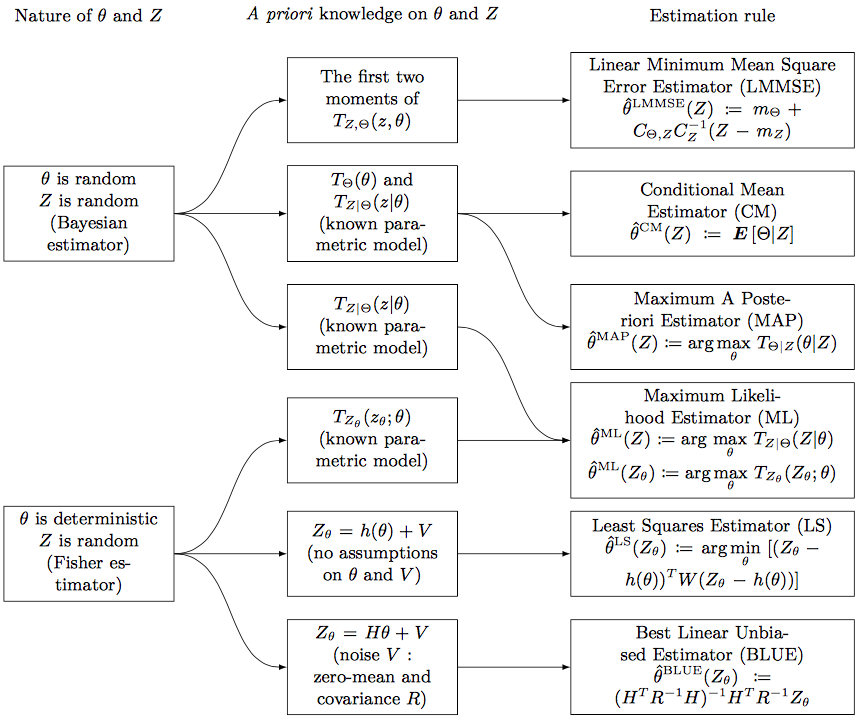
\includegraphics[width=\textwidth]{img/estsumm}
	\caption{Résumé des différents estimateurs.}
	\label{fig:estsumm}
\end{figure}

\section{Filtrage et prédiction}
\subsection{Analyse de systèmes dynamiques}
\subsubsection{Problème de filtrage non linéaire}
\begin{myprob}[Problème de filtrage non linéaire]
Soit le vecteur d'état \(x_t \in \Rm\) et
le vecteur d'observation \(y_t \in \Rn\).
On suppose que ces vecteurs satisfont les équations suivantes:
\begin{align}
	x_{t+1} &= F(x_t) + \Gamma u_t\,,\label{eq:state}\\
	y_t &= G(x_t) + w_t\,.\label{eq:observation}
\end{align}

\eqref{eq:state} est l'\emph{équation d'état} et
modélise l'évolution de l'état au cours du temps.
Ici, \(F \colon \Rm \to \Rm\) est une fonction donnée,
\(\Gamma\) est une matrice \(m \times m\) donnée et
\(u_t \in \Rm\) est un vecteur de variables de perturbation (bruit).
Si l'on suppose que les \(u_t\)s sont indépendants,
alors le processus résultant \(x_t\) est un processus de Markov:
\begin{equation}
	\pdf(x_t \mid x_1, \ldots, x_{t-1}) = \pdf(x_t \mid x_{t-1})\,.
\end{equation}

\eqref{eq:observation} est l'\emph{équation d'observation} et
donne le lien entre l'état \(x_t\) et l'observation \(y_t\).
Ici, \(G \colon \Rm \to \Rn\) est une fonction donnée et
\(w_t \in \Rn\) est un vecteur de bruit d'observation.
On suppose que \(w_t\) est indépendant au travers du temps,
c'est-à-dire que \(w_t\) est indépendant de \(w_s\), pour \(s \ne t\),
et est également indépendant de \(x_t\) et \(u_t\).
On a donc
\begin{equation}
	\pdf(y_t \mid y_1, \ldots, y_{t-1}, x_t) = \pdf(y_t \mid x_t)\,.
\end{equation}

En combinant ces équations, on trouve la densité à posteriori de \(x_t\) comme
\begin{align}
	\pdf(x_t \mid y_1, \ldots, y_t) &= \frac{\pdf(x_t, y_1, \ldots, y_t)}{\pdf(y_1, \ldots, y_t)}\\
	&= \frac{\pdf(y_t \mid x_t, y_1, \ldots, y_{t-1}) \pdf(x_t \mid y_1, \ldots, y_{t-1}) \pdf(y_1, \ldots, y_{t-1})}{\pdf(y_t \mid y_1, \ldots, y_{t-1}) \pdf(y_1, \ldots, y_{t-1})}\,,
	\intertext{par la formule des probabilités totales, et donc}
	&= \frac{\pdf(y_t \mid x_t) \pdf(x_t \mid y_1, \ldots, y_{t-1})}{\pdf(y_t \mid y_1, \ldots, y_{t-1})}\,,
	\intertext{par la propriété de Markov.}
\end{align}
En étudiant le terme de droite dans le numérateur, on trouve
\begin{align}
	\pdf(x_t \mid y_1, \ldots, y_{t-1}) &= \int_{x_{t-1}} \pdf(x_t, x_{t-1} \mid y_1, \ldots, y_{t-1}) \dif x_{t-1}\\
	&= \int_{x_{t-1}} \pdf(x_t \mid x_{t-1}) \pdf(x_{t-1} \mid y_1, \ldots, y_{t-1}) \dif x_{t-1}\,.
\end{align}
Ceci donne lieu aux deux équations de filtrage non linéaire:
\begin{align}
	\pdf(x_t \mid y_1, \ldots, y_{t-1}) &= \int_{x_{t-1}} \pdf(x_t \mid x_{t-1}) \pdf(x_{t-1} \mid y_1, \ldots, y_{t-1}) \dif x_{t-1}\,,\label{eq:prediction}\\
	\pdf(x_t \mid y_1, \ldots, y_{t-1}) &= \frac{\pdf(y_t \mid x_t) \pdf(x_t \mid y_1, \ldots, y_{t-1})}{\pdf(y_t \mid y_1, \ldots, y_{t-1})}\,.\label{eq:correction}
\end{align}
\eqref{eq:prediction} est appelée l'\emph{équation de prédiction},
car elle utilise les données passées \(y_1, \ldots, y_{t-1}\)
pour prédire un état futur \(x_t\).
Cette équation utilise deux densités de probabilité:
\begin{itemize}
	\item la densité à posteriori de \(x_{t-1}\),
	connaissant toutes les données passées et
	\item la prédiction de \(x_t\) en connaissant \(x_{t-1}\).
\end{itemize}
Les données en \(t\), \(y_t\),
ne jouent pas de rôle dans l'équation de prédiction.
Ces données entrent dans \eqref{eq:correction},
qui utilise également deux densités de probabilité:
\begin{itemize}
	\item la densité de prédiction à posteriori
	\(\pdf(x_t \mid y_1, \ldots, y_{t-1})\),
	obtenue à partir de l'équation de prédiction et
	\item la fonction de vraisemblance pour les données en \(t\),
	donnée par \(\pdf(y_t \mid x_t)\).
\end{itemize}

Le problème du filtrage bayésien non linéaire est celui
d'estimer la valeur en \(t\) à partir de la densité à posteriori.
Plusieurs estimateurs peuvent être utilisés; par exemple:
\begin{itemize}
	\item l'estimateur MAP étant donné toutes les données jusqu'en \(t\),
	\begin{equation}
		\xhat_t^{\textnormal{MAP}} = \argmax_{x_t} \pdf(x_t \mid y_1, \ldots, y_t)\,;
	\end{equation}
	\item l'estimateur de la moyenne à posteriori,
	\begin{equation}
		\xhat_t^\mu = \int_{x_t} x_t \pdf(x_t \mid y_1, \ldots, y_t) \dif x_t\,.
	\end{equation}
	\item l'estimateur de la médiane à posteriori, etc.
\end{itemize}
En plus d'estimer \(x_t\), on s'intéresse également
à la qualité de l'estimateur.
On doit donc aussi estimer la variance de \(x_t\) sous la densité à posteriori,
\(\pdf(x_t \mid y_1, \ldots, y_t)\).
\end{myprob}

\subsection{Méthodes de Monte-Carlo séquentielles}
Soit \(\pdf(x_t \mid y_1, \ldots, y_t)\)
la densité de probabilité à postériori au temps \(t\)
et soit \(x_t^i\) un échantillon de cette densité.
Définissons l'ensemble des échantillons
\(S_t = \{\,x_t^i\,,\quad i = 1, \ldots, n\,\}\)\,.
Notre but est d'utiliser les éléments de \(S_t\),
la nouvelle observation \(y_{t+1}\) et
les modèles du système-observation afin de générer \(S_{t+1}\).
En utilisant les équations de filtrage non linéaire
\eqref{eq:prediction} et \eqref{eq:correction},
ceci se fait en deux étapes.
La première étape génère une prédiction,
et la deuxième étape corrige celle-ci
en utilisant la donnée \(y_{t+1}\).
\begin{enumerate}
	\item \emph{Étape de prédiction}:
	cette étape utilise les échantillons de la densité en \(t\)
	afin de générer des échantillons de la densité de prédiction
	\(\pdf(x_{t+1} \mid y_1, \ldots, y_t)\).
	L'idée de base est d'interpréter \eqref{eq:prediction}
	comme une densité de mélange.
	\begin{equation}
		\pdf(x_{t+1} \mid y_1, \ldots, y_t) = \int_{x_t} \pdf(x_{t+1} \mid x_t) \pdf(x_t \mid y_1, \ldots, y_t) \dif x_t\,.
	\end{equation}
	Comme \(x_t^i\) est un échantillon
	de \(\pdf(x_t \mid y_1, \ldots, y_t)\),
	on peut utiliser un échantillon
	de la densité conditionnelle \(\pdf(x_{t+1} \mid x_t^i)\).
	La valeur \(\xtil_t^i \sim \pdf(x_{t+1} \mid x_t^i)\)
	est un échantillon \(\pdf(x_{t+1} \mid y_1, \ldots, y_t)\).
	On appelle l'ensemble
	\(\tilde{S}_{t+1} = \{\,\xtil_t^1, \ldots, \xtil_t^n\,\}\)
	l'\emph{ensemble de prédiction}.
	Si nécessaire,
	on peut estimer les moments en utilisant cet ensemble:
	\begin{equation}
		\hat{\mu}_{t+1 \mid t} = \frac{1}{n} \sum_{i=1}^n \xtil_t^i\,.
	\end{equation}

	Cette étape n'utilise pas les nouvelles données \(y_{t+1}\),
	et son succès dépend de notre capacité
	à échantillonner à partir de \(\pdf(x_{t+1} \mid x_t^i)\).
	Comme dit par \eqref{eq:state},
	cette densité provient de l'équation d'état,
	utilisant une fonction de correction \(F\) et
	un terme aléatoire \(\Gamma u_t\).
	On peut donc échantillonner avec
	\begin{equation}
		\xtil_{t+1}^i = F(x_t^i) + \Gamma u_t^i\,,
	\end{equation}
	où \(u_t^i\) est un échantillon aléatoire.
	\item \emph{Étape de correction}:
	cette étape utilise \eqref{eq:observation} et
	l'ensemble de prédiction \(\tilde{S}_{t+1}\)
	afin de générer des échantillons
	de la densité à posteriori \(\pdf(x_{t+1} \mid y_1, \ldots, y_{t+1})\).
	En plus, on veut estimer un paramètre
	\begin{equation}
		\theta_{t+1} = \int g(x_{t+1}) \pdf(x_{t+1} \mid y_1, \ldots, y_{t+1}) \dif x_{t+1}\,,
	\end{equation}
	pour une fonction donnée \(g\).
	Dans le cas d'estimation MMSE,
	la fonction \(g\) est l'indentité,
	et on veut estimer la moyenne à posteriori
	comme une estimée de l'état \(x_{t+1}\).
	Cependant, sous d'autres critères d'estimation,
	\(g\) peut être différente, mais toujours connue à l'avance.
	Ces deux buts sont accomplis
	en utilisant l'\emph{échantillonage préférentiel}
	et le \emph{ré-échantillonnage}, comme suit.

	D'abord, on considère le but d'estimer \(\theta_{t+1}\).
	On peut écrire
	\begin{align}
		\theta_{t+1} &= \int g(x_{t+1}) \pdf(x_{t+1} \mid y_1, \ldots, y_{t+1}) \dif x_{t+1}\\
		&= \int g(x_{t+1}) \frac{\pdf(y_{t+1} \mid x_{t+1}) \pdf(x_{t+1} \mid y_1, \ldots, y_t)}{\pdf(y_{t+1} \mid y_1, \ldots, y_t)} \dif x_{t+1}\\
		&= \int \left(\frac{g(x_{t+1}) \pdf(y_{t+1} \mid x_{t+1})}{\pdf(y_{t+1} \mid y_1, \ldots, y_t)}\right) \pdf(x_{t+1} \mid y_1, \ldots, y_t) \dif x_{t+1}\,.\label{eq:smctheta}
	\end{align}
	Le deuxième terme vient directement
	par application de \eqref{eq:correction}.
	Maintenant qu'on a des échantillons de
	\(\pdf(x_{t+1} \mid y_1, \ldots, y_t)\)
	(dans l'ensemble \(\tilde{S}_{t+1}\)),
	on peut les utiliser pour estimer \(\theta_{t+1}\).
	Ceci requiert l'évaluation de l'expression entre parenthèses
	sur ces échantillons et
	puis de prendre la moyenne sur \(n\) échantillons.
	Pour ceci, on a besoin de la densité inconnue
	\(\pdf(y_{t+1} \mid y_1, \ldots, y_t)\).
	On doit donc l'estimer également afin d'estimer \(\theta_{t+1}\)
	par échantillonnage préférentiel.
	On fait ceci en considérant
	\begin{equation}
		\pdf(y_{t+1} \mid y_1, \ldots, y_t) = \int \pdf(y_{t+1} \mid x_{t+1}) \pdf(x_{t+1} \mid y_1, \ldots, y_t) \dif x_{t+1}\,.
	\end{equation}
	Afin d'estimer la quantité à gauche,
	on peut utiliser les échantillons de
	\(\pdf(x_{t+1} \mid y_1, \ldots, y_t)\)
	et la fonction de vraisemblance \(\pdf(y_{t+1} \mid x_{t+1})\).
	Définissons les poids
	\begin{equation}
		w_{t+1}^i = \pdf(y_{t+1} \mid \xtil_{t+1}^i)
	\end{equation}
	et estimons \(\pdf(y_{t+1} \mid y_1, \ldots, y_t)\)
	avec \(\frac{1}{n} \sum_{i=1}^n w_{t+1}^i\).
	Ceci est l'idée classique de Monte-Carlo.
	On trouve donc maintenant, en combinant ceci avec \eqref{eq:smctheta},
	\begin{equation}
		\htheta_{t+1} = \frac{1}{n} \sum_{i=1}^n \left( \frac{g(\xtil_{t+1}^i) w_{t+1}^i}{\frac{1}{n} \sum_{j=1}^n w_{t+1}^j} \right)\,.
	\end{equation}
	On peut réécrire ceci avec des poids normalisés
	\(\tilde{w}_{t+1}^i = \frac{w_{t+1}^i}{\sum_{j=1}^n w_{t+1}^i}\) comme
	\begin{equation}
		\htheta_{t+1} = \sum_{i=1}^n g(\xtil_{t+1}^i) \tilde{w}_{t+1}^i\,.
	\end{equation}
	Maintenant, on se préoccupe den nouveau avec
	la génération des échantillons de la densité à posteriori,
	\(\pdf(x_{t+1} \mid y_1, \ldots, y_{t+1})\).
	On peut montrer qu'en ré-échantillonnant à partir de \(\tilde{S}_{t+1}\)
	avec des probabilités données par
	\begin{equation}
		\{\,\tilde{w}_{t+1}^1, \ldots, \tilde{w}_{t+1}^n\,\}\,,
	\end{equation}
	alors les valeurs résultantes sont des échantillons
	de la densité à posteriori.
	En générant \(n\) échantillons \(x_{t+1}^1, \ldots, x_{t+1}^n\),
	on obtient l'ensemble
	\begin{equation}
		S_{t+1} = \{\,x_{t+1}^1, \ldots, x_{t+1}^n\,\}\,.
	\end{equation}
\end{enumerate}

\begin{myalgo}[SMC classique]
	\leavevmode
	\begin{enumerate}
		\item Générer \(n\) échantillons \(x_0^i \sim \pdf(x_0)\),
		et poser \(t \coloneqq 0\).
		\item \label{step:smc2} \emph{Prédiction}:
		Générer l'ensemble de prédiction en utilisant
		\begin{equation}
			\xtil_{t+1}^i \sim \pdf(x_{t+1} \mid x_t^i)\,, \quad i = 1, \ldots, n\,.
		\end{equation}
		\item \emph{Correction}:
		Calculer les poids
		\begin{equation}
			w_{t+1}^i = \pdf(y_{t+1} \mid \xtil_{t+1})
		\end{equation}
		et les normaliser avec
		\(\tilde{w}_{t+1}^i =\frac{w_{t+1}^i}{\sum_{j=1}^n w_{t+1}^i}\).
		\begin{enumerate}
			\item Estimer \(\theta_{t+1}\)
			avec \(\htheta_{t+1} = \sum_{i=1}^n g(\xtil_{t+1}^i) \tilde{w}_{t+1}^i\).
			\item Ré-échantillonner à partir de l'ensemble
			\(\xtil_{t+1}^1, \ldots, \xtil_{t+1}^n\)
			avec les probabilités
			\(\tilde{w}_{t+1}^1, \ldots, \tilde{w}_{t+1}^n\),
			\(n\) fois, afin d'obtenir les échantillons
			\(x_{t+1}\), \(i = 1, \ldots, n\).
		\end{enumerate}
		\item Mettre \(t \coloneqq t+1\),
		et retourner à l'étape~\ref{step:smc2}.
	\end{enumerate}
\end{myalgo}

Il est possible que le ré-échantillonnage donne lieu
à un faible nombre de valeurs distinctes dans \(S_{t+1}\).
Bien que ces valeurs soient valables,
elles peuvent conduire à un mauvais estimateur pour \(\theta_{t+1}\).
On peut, le cas échéant,
remplacer les \(x_{t+1}^i\) par des autres valeurs,
trouvées en partant de \(x_{t+1}^i\)
avec un algorithme MCMC\footnote{Monte-Carlo par chaînes de Markov.}
tel que l'algorithme de Metropolis-Hastings.

\subsection{Filtre de Wiener}
Le filtre de Wiener permet,
pour deux signaux conjointement stationnaires \(X[k]\) et \(Y[k]\),
de construire une estimée \(\xhat[k]\) de \(x[k]\)
à partir d'un échantillon de mesures bruitées \(y[j]\):
\begin{equation}
	\xhat[k] = \sum_{\ell = \ell_1}^{\ell_2} w[\ell] y[k - \ell]\,.
\end{equation}
Les coefficients \(w[\ell]\) sont calculés
de manière à minimiser l'erreur quadratique moyenne d'estimation \(\xi\):
\begin{equation}
	\xi = \expe{\abs{E[k]}^2} = \expe{\abs{X[k] - \hat{X}[k]}^2}\,.
\end{equation}
L'hypothèse requise pour la construction d'un filtre de Wiener est que
le processus stochastique \(Z[k] = (X[k], Y[k])^T\) soit WSS.
On peut donc définir la fonction matricielle de covariance et la PSD matricielle
du processus \(Z[k]\).
Le filtre peut se calculer à partir de celles-ci.
C'est l'information contenue
dans la covariance (ou PSD) mutuelle de \(X\) et \(Y\)
qui permet d'estimer \(\xhat\) à partir de \(y\).
Il existe plusieurs variantes du problème de Wiener
suivant quelles observations \(y[j]\) on utilise pour estimer \(x[k]\),
chacun avec son filtre d'estimation propre:
\begin{itemize}
	\item \emph{Filtrage}: jusqu'à l'instant \(j = k\), avec le filtre
	\begin{equation}
		\xhat[k] = \sum_{\ell = 0}^{\ell_2} w[\ell] y[k - \ell]\,, \quad \ell_2 > 0\,.
	\end{equation}
	\item \emph{Prédiction}: jusqu'à un instant antérieur \(j < k\),
	avec le filtre
	\begin{equation}
		\xhat[k] = \sum_{\ell = \ell_1}^{\ell_2} w[\ell] y[k - \ell]\,, \quad 0 < \ell_1 < \ell_2\,.
	\end{equation}
	\item \emph{Lissage}: jusqu'à un instant postérieur \(j > k\),
	avec le filtre
	\begin{equation}
		\xhat[k] = \sum_{\ell = \ell1}^{\ell_2} w[\ell] y[k - \ell]\,, \quad \ell_1 < 0 < \ell_2\,.
	\end{equation}
\end{itemize}
Dans le cas du filtrage et de la prédiction,
le filtre est causal, mais pas pour le lissage.
En effet, il faut attendre jusqu'à l'instant \(k - \ell_1 > k\)
pour estimer \(\xhat[k]\).

\subsubsection{Filtre de Wiener FIR}
On veut construire \(\xhat[k]\)
par traitement linéaire des observations \(\{\,y[k]\,, j \le k\,\}\)
à l'aide d'un filtre FIR (à réponse impulsionnelle finie) \(w\).

Pour un filtre d'ordre \(N-1\), l'estimateur est donné par
\begin{equation}
	\xhat[k] = \sum_{\ell = 0}^{N-1} w[\ell] y[k - \ell]\,.
\end{equation}
Le filtre de Wiener est celui qui minimise \(\xi\).
Pour que ce filtre soit optimal,
il faut que le gradient par rapport aux coefficients (complexes) du filtre
soit nul; il s'agit d'une fonction réelle de \(2N\) variables réelles.
En notant \(w[\ell] = \wienr[\ell] + \imagj \wieni[\ell]\), on requiert que
\begin{align}
	\fpart{\xi}{\wienr[\ell]} &= 0\,, \quad \ell = 0, \ldots, N - 1\,,\\
	\fpart{\xi}{\wieni[\ell]} &= 0\,, \quad \ell = 0, \ldots, N - 1\,.
\end{align}
On doit également s'assurer que les derivés secondes soient positives,
afin d'avoir un minimum.
On trouve
\begin{align}
	\fpart{\xi}{\wienr[\ell]} &= \fpart{\expe{\abs{E[k]}^2}}{\wienr[\ell]}\\
	&= \fpart{\expe{E[k] E^*[k]}}{\wienr[\ell]}\\
	&= \expe{\fpart{E[k]}{\wienr[\ell]} E^*[k]} + \expe{E[k] \fpart{E^*[k]}{\wienr[\ell]}}\\
	&= \expe{-Y[k - \ell] E^*[k]} + \expe{-Y^*[k - \ell] E[k]}\\
	&= 2 \expe{\Re(-Y^*[k - \ell] E[k])} = 0\,,\\
	\frac{\partial^2 \xi}{\partial \wienr^2[\ell]} &= 2 \expe{\Re(-Y^*[k - \ell] \fpart{E[k]}{\wienr[\ell]})}\\
	&= 2 \expe{Y^*[k - \ell]Y[k - \ell]} > 0\,.
	\intertext{Le raisonnement pour la deuxième condition
	se dérive de façon semblable:}
	\fpart{\xi}{\wieni[\ell]} &= 2 \expe{\Im(-Y^*[k - \ell] E[k])} = 0\,,\\
	\frac{\partial^2 \xi}{\partial \wienr^2[\ell]} &=  2 \expe{Y^*[k - \ell]Y[k - \ell]} > 0\,.
\end{align}
En combinant ces conditions en une,
on trouve le \emph{principe d'orthogonalité}
(ou \emph{théorème de projection}) suivant:
\begin{equation}
	\fpart{\xi}{\wienr[\ell]} + \imagj \fpart{\xi}{\wieni[\ell]} = \expe{E[k] Y^*[k - \ell]} = 0\,, \quad \ell = 0, \ldots, N-1\,.
\end{equation}
Il s'écrit aussi
\begin{equation}
		\fpart{\xi}{w^*[\ell]} = 0\,, \quad \textnormal{avec } \fpart{}{w^*[\ell]} = \fpart{}{\wienr[\ell]} + \imagj \fpart{}{\wieni[\ell]}\,.
\end{equation}
Ce principe signifie que
si la solution est optimale au sens de la minimisation de la MSE,
alors l'erreur d'estimation est orthogonale aux observations.
Un corollaire de ceci est que la corrélation mutuelle \(R_{\hat{X} E}(0)\)
entre l'estimation obtenue par la solution optimale et
l'erreur d'estimation correspondante est nulle:
\begin{align}
	R_{\hat{X} E}(0) &= \expe{\hat{X}[k] E[k]}\\
	&= \sum_{i=0}^{N-1} w[\ell] \expe{Y[k - \ell] E^*[k]}
	\intertext{et en appliquant le principe d'orthogonalité}
	&= 0\,.
\end{align}

Une autre conséquence du principe d'orthogonalité
se trouve en remplaçant \(E\) par sa valeur
\(X[k] - \hat{X}[k] = X[k] - \sum_{j=0}^{N-1} w[j] Y[k - j]\):
\begin{align}
	\expe{X[k] Y^*[k -\ell]} &= \expe{\hat{X}[k] Y^*[k - \ell]}\\
	&= \sum_{j=0}^{N-1} w[j] \expe{Y[k - j] Y^*[k - \ell]}\\
	\iff R_{XY}(\ell) &= \sum_{j=0}^{N-1} w[j] R_Y(\ell - j)\,.
\end{align}
Cet ensemble d'équations, pour \(0 \le \ell \le N-1\),
porte le nom d'\emph{équations de Wiener-Hopf}.
En utilisant le fait que la fonction de corrélation est hermitienne,
\(R_Y(-k) = R_Y^*(k)\), on peut expliciter cela sous la forme
\begin{equation}
	\begin{pmatrix}
		R_Y(0) & R_Y^*(1) & \cdots & R^*_Y(N - 1)\\
		R_Y(1) & R_Y^*(0) & \cdots & R^*_Y(N - 2)\\
		\vdots & \ddots & \ddots & \vdots\\
		R_Y(N - 1) & \cdots & \cdots & R_Y(0)
	\end{pmatrix}
	\begin{pmatrix} w[0] \\ w[1] \\ \vdots \\ w[N - 1] \end{pmatrix}
	=
	\begin{pmatrix} R_{XY}(0) \\ R_{XY}(1) \\ \vdots \\ R_{XY}(N - 1) \end{pmatrix}\,,
\end{equation}
ou encore
\begin{equation}
	R_Y w = R_{XY}
	\iff w_{\textnormal{opt}} = R_Y^{-1} R_{XY}\,,
\end{equation}
où la solution optimale \(w_{\textnormal{opt}}\)
définit les coefficients du filtre de Wiener.

Le critère \(\xi\) vaut
\begin{align}
	\xi &= \expe{E[k] E^*[k]}\\
	&= \expe{E[k] X^*[k]} - \underbrace{\expe{E[k]\hat{X}^*[k]}}_{0}\,.
	\intertext{Par le principe d'orthogonalité, le terme de droite est nul:}
	\xi &= \expe{X[k] X^*[k]} - \sum_{\ell = 0}^{N - 1} w[\ell] \expe{Y[k - \ell] X^*[k]}\\
	&= R_X(0) - w^T R^*_{XY}\,.
	\intertext{Quand le filtre est optimal, cela devient}
	\xi_{\min} &= R_X(0) - R^T_{XY} R_Y^{-T} R^*_{XY}\,.\label{eq:ximin}
\end{align}
On développe ensuite \(\xi\)
\begin{align}
	\xi &= \expe{E[k] E^*[k]}\\
	&= \expe{\left(X[k] - \sum_{\ell = 0}^{N-1} w[\ell] Y[k - \ell]\right)\left(X^*[k] - \sum_{\ell' = 0}^{N-1} w^*[\ell'] Y^*[k - \ell']\right)}\\
	&= \begin{multlined}[t]
	R_X(0) - \sum_{\ell' = 0}^{N - 1} w^*[\ell'] \expe{X[k] Y^*[k - \ell']} - \sum_{\ell = 0}^{N - 1} w[\ell] \expe{X^*[k] Y[k - \ell]}\\ {} + \sum_{\ell = 0}^{N - 1} \sum_{\ell' = 0}^{N - 1} w[\ell] w^*[\ell] \expe{Y[k - \ell] Y^*[k - \ell']}
	\end{multlined}\\
	&= R_X(0) - w^\dag R_{XY} - R^\dag_{XY} w + w^\dag R_Y w\,,
\end{align}
où \(w^\dag\) est le vecteur transposé et conjugué de \(w\).
Pour le filtre optimal \(w = w_{\textnormal{opt}} = R_Y^{-1} R_{XY}\),
les trois derniers termes sont identiques (sans le signe),
et on retrouve \eqref{eq:ximin}.
La surface d'erreur apparaît comme une fonction quadratique
des coefficients du filtre, et a donc un minimum unique.
En utilisant \(R_{XY} = R_Y w_{\textnormal{opt}}\),
on peut encore exprimer le critère comme
\begin{equation}
	\xi = \xi_{\min} + (w - w_{\textnormal{opt}})^\dag R_Y (w - w_{\textnormal{opt}})\,.
\end{equation}
On peut diagonaliser \(R_Y\) avec la matrice \(\Lambda\)
des valeurs propres \(\lambda_k\)
et la matrice orthonormale des vecteurs propres \(M\):
\begin{align}
	R_Y &= M \Lambda M^\dag\\
	\iff \xi &= \xi_{\min} + (w - w_{\textnormal{opt}})^\dag M \Lambda M^\dag (w - w_{\textnormal{opt}})\\
	&= \xi_{\min} + \nu^\dag \Lambda \nu\\
	&= \xi_{\min} + \sum_{k} \lambda_k \abs{v}^2\,.
\end{align}
Cela revient à formuler le problème dans un système d'axes
qui est celui des axes principaux de la surface d'erreur.
Comme les valeurs propres sont positives ou nulles,
on voit que la surface d'erreur est une paraboloïde elliptique.
La contribution au critère due à l'erreur
commise sur chaque composante apparaît clairement.
On a \og orthogonalisé \fg{} le problème.

Considérons le modèle suivant: \(Y[k] = X[k] + V[k]\),
où \(V[k]\) est un bruit centré et non corrélé avec \(X\).
En utilisant le fait que
\begin{align}
	R_{XY}(k) &= \expe{X[n] Y^*[n - k]}\\
	&= \expe{X[n] X[n - k]} + \expe{X[n] V[n-k]}\\
	&= R_X(k)\,,\\
	R_Y(k) &= R_X(k) + R_V(k)\,.
\end{align}
On peut donc particulariser les équations de Wiener-Hopf comme
\begin{align}
	(R_X + R_V) w = R_X\,.
\end{align}

\subsubsection{Prédicteur de Wiener FIR}
On souhaite maintenant construire un prédicteur optimal de Wiener à horizon 1,
c'est-à-dire construire un estimateur linéaire de \(\xhat[k+1]\)
en utilisant toutes les observations \(\{\,y[j]\,, j \le k\,\}\)
d'un signal \(Y\) corrélé avec le signal \(X\).
Cet estimateur prend donc la forme
\begin{equation}
	\xhat[k+1] = \sum_{\ell = 0}^{N - 1} w[\ell] y[k - \ell]\,.
\end{equation}
En utilisant le principe d'orthogonalité, on trouve
\begin{align}
	\expe{X[k+1] Y^*[k - \ell]} &= \expe{\hat{X}[k+1] Y^*[k - \ell]}\\
	&= \sum_{j = 0}^{N - 1} w[j] \expe{Y[k - j] Y^*[k - \ell]}\\
	\implies R_{XY}(\ell + 1) &= \sum_{j=0}^{N - 1} w[j] R_Y(\ell - j)\,.
\end{align}
On trouve encore une fois les \emph{équations de Wiener-Hopf}:
\begin{equation}
	\begin{pmatrix}
		R_Y(0) & R_Y^*(1) & \cdots & R^*_Y(N - 1)\\
		R_Y(1) & R_Y^*(0) & \cdots & R^*_Y(N - 2)\\
		\vdots & \ddots & \ddots & \vdots\\
		R_Y(N - 1) & \cdots & \cdots & R_Y(0)
	\end{pmatrix}
	\begin{pmatrix} w[0] \\ w[1] \\ \vdots \\ w[N - 1] \end{pmatrix}
	=
	\begin{pmatrix} R_{XY}(1) \\ R_{XY}(2) \\ \vdots \\ R_{XY}(N) \end{pmatrix}\,,
\end{equation}
ou encore
\begin{equation}
	R_Y w = R_{XY}^1\,,
\end{equation}
où l'exposant \(1\) indique la profondeur de l'horizon de prédiction.
Si on avait utilisé une somme pour \(\ell = 1\) jusque \(N\),
on aurait trouvé le même résultat, mais avec les coefficients du filtre décalés
(\(w[1]\) jusque \(w[N]\) au lieu de \(w[0]\) jusque \(w[N - 1]\)).

Supposons maintenant que \(X[k] = Y[k]\),
c'est-à-dire qu'on veut prédire le signal dont on dispose.
Les équations de Wiener-Hopf deviennent (en utilisant la somme de \(1\) à \(N\))
\begin{equation}
	\begin{pmatrix}
		R_Y(0) & R_Y^*(1) & \cdots & R^*_Y(N - 1)\\
		R_Y(1) & R_Y^*(0) & \cdots & R^*_Y(N - 2)\\
		\vdots & \ddots & \ddots & \vdots\\
		R_Y(N - 1) & \cdots & \cdots & R_Y(0)
	\end{pmatrix}
	\begin{pmatrix} w[1] \\ w[2] \\ \vdots \\ w[N] \end{pmatrix}
	=
	\begin{pmatrix} R_Y(1) \\ R_Y(2) \\ \vdots \\ R_Y(N) \end{pmatrix}\,,
\end{equation}
ou encore
\begin{equation}
	R_Y w = R_Y^1\,,
\end{equation}

\paragraph{Prédiction linéaire à partir de données bruitées}
Supposons que l'on dispose de \(Y[j] = X[j] + V[j]\),
où \(V\) est un bruit perturbateur décorrélé.
On souhaite estimer \(X[n]\), avec \(j < n\).
\begin{align}
	\expe{X[k] Y^*[k - \ell]} &= \expe{X[k] Y^*[k - \ell]}\\
	&= \expe{X[k] X^*[k - \ell]} + \expe{X[k] V^*[k - \ell]}\\
	&= R_X[\ell]\,,
\end{align}
pour \(\ell = 1, \ldots, N\).
On trouve aussi
\begin{align}
	\expe{Y[k - j] Y^*[k - \ell]} &= R_Y(\ell - j)\\
	&= \expe{X[k - j] X^*[k - \ell]} + \expe{V[k - j] V^*[k - \ell]}\\
	&= R_X(\ell - j) + R_V(\ell - j)\,.
\end{align}
Les équations de Wiener-Hopf deviennent alors
\begin{equation}
	(R_X + R_V) w = R_X^1\,.
\end{equation}
Si le bruit est de plus blanc et de variance \(\vars_V\), on a encore
\begin{equation}
	R_Y = R_X + R_V = R_X + \vars_V I\,,
\end{equation}
où \(I\) est la matrice unité.
Les équations deviennent donc
\begin{equation}
	(R_X + \vars_V I) w = R_X^1\,.
\end{equation}
Cet estimateur, appelé \emph{prédicteur à horizon 1},
permet d'estimer un signal en \(n\)
à partir de la connaissance dont on dispose jusque \(n-1\).
Pour la prédiction à horizon \(n_0\),
à savoir la prédiction de \(Y[n + n_0 - 1]\)
à partir de la connaissance dont on dispose jusque \(n-1\),
le raisonnement est similaire.

\subsubsection{Filtre de Wiener IIR non causal: lissage optimal}
On prend
\begin{equation}
	\hat{X}(n) = \sum_{\ell = -\infty}^{+\infty} w(\ell) Y(n - \ell)\,.
\end{equation}
Les équations de Wiener-Hopf deviennent alors
\begin{equation}
	\sum_{\ell = -\infty}^{+\infty} w(\ell) R_Y(k - \ell) = R_{XY}(k)\,, \quad -\infty \le k \le + \infty\,.
\end{equation}
Il s'agit donc d'un opérateur de lissage.
En prenant la transformée de Fourier et en réalisant
que le premier membre est une convolution, il vient
\begin{equation}
	W(\e^{\imagj \Omega}) \gamma_Y(\e^{\imagj \Omega}) = \gamma_{XY}(\e^{\imagj \Omega})\,,
\end{equation}
et donc
\begin{equation}
	W_{\textnormal{opt}}(\e^{\imagj \Omega}) = \frac{\gamma_{XY}(\e^{\imagj \Omega})}{\gamma_Y(\e^{\imagj \Omega})}\,.
\end{equation}

L'erreur quadratique moyenne \(\xi\) est donnée par
\begin{align}
	\xi &= \expe{E(n)X^*(n)}\\
	&= \expe{X(n) X^*(n)} - \sum_{\ell = -\infty}^{+\infty} w(\ell) \expe{Y(n-\ell) X^*(n)}\\
	&= R_X(0) - \sum_{\ell=-\infty}^{+\infty} w(\ell) R_{YX}(-\ell)\\
	&= R_X(0) - \sum_{\ell = -\infty}^{+\infty} w(\ell) R_{XY}^*(\ell)\\
	&= R_X(0) - \frac{1}{2\pi} \int_0^{2\pi} W(\e^{\imagj \Omega}) \gamma_{XY}^*(\e^{\imagj \Omega}) \dif \Omega\,.
	\intertext{Si le filtre est optimal, on trouve}
	\xi_{\textnormal{min}} &= R_X(0) - \frac{1}{2\pi} \int_0^{2\pi} \frac{\gamma_{XY}(\e^{\imagj \Omega})}{\gamma_Y(\e^{\imagj \Omega})} \gamma_{XY}^*(\e^{\imagj \Omega}) \dif \Omega\\
	&= R_X(0) - \frac{1}{2\pi} \int_0^{2\pi} \frac{\abs{\gamma_{XY}(\e^{\imagj \Omega})}^2}{\gamma_Y(\e^{\imagj \Omega})} \dif \Omega\,.
\end{align}

\subsubsection{Filtre de Wiener IIR causal: filtrage optimal}
On prend
\begin{equation}
	\hat{X}(n) = \sum_{\ell = 0}^{+\infty} w(\ell) Y(n - \ell)\,.
\end{equation}
Les équations de Wiener-Hopf deviennent alors
\begin{equation}
	\sum_{\ell = 0}^{+\infty} w(\ell) R_Y(k - \ell) = R_{XY}(k)\,, \quad 0 \le k \le +\infty\,.
\end{equation}
Il faudrait utiliser ici une transformée de Fourier unilatérale
pour copier le raisonnement pour le lissage optimal.
On peut cependant utiliser le théorème de factorisation spectrale,
qui dit que tout processus stationnaire comme \(Y(n)\)
peut être représenté de façon équivalente par passage
d'un bruit blanc d'innovation \(I(n)\) de variance \(\vars_I\)
dans un filtre \(h(n)\) monique, causal et stable à phase minimale tel que
\begin{equation}
	\gamma_Y(\ejw) = \vars_I \abs{H(\ejw)}^2\,.
\end{equation}
Supposons \(I(n)\) correspondant au blanchiment de \(Y(n)\).
On peut résoudre le problème d'estimation de \(X(n)\) à partir de \(I(n)\),
plutôt que de \(Y(n)\) et de trouver le filtre \(w_{\textnormal{i}}\)
agissant sur \(I(n)\) qui minimise le critère.
Les équations de Wiener-Hopf sont alors
\begin{align}
	\sum_{\ell = 0}^{+\infty} w_{\textnormal{i}}(\ell) R_I(k - \ell) &= R_{XI}(k)\,.
	\intertext{Sachant que \(I(n)\) est un bruit blanc,}
	\sum_{\ell = 0}^{+\infty} w_{\textnormal{i}}(\ell) \vars_I \delta(k - \ell) &= \vars_I w_{\textnormal{i}}(k)\\
	&= R_{XI}(k)\,.
\end{align}
Le filtre d'estimation est donc égal à la partie causale
de la séquence de corrélation mutuelle divisée par
la variance du bruit blanc.
On écrit aussi que la transmittance du filtre est donnée par
la transformée de Fourier de la partie causale de la séquence, et on note
\begin{equation}
	W_{\textnormal{i}}(\ejw) = \frac{1}{v\vars_I}\gamma_{XI}(\ejw)|_{+}\,.
\end{equation}
Or le filtre qu'on recherche est celui permettant de calculer
l'estimation à partir de \(Y(n)\):
\begin{equation}
	\hat{X}(n) = \wi(n) \ast I(n)\,.
\end{equation}
On peut également trouver le filtre de blanchiment
causal et stable associé à \(Y(n)\).
Si \(h(n)\) est à phase minimale, alors le filtre \(\ell(n)\)
dont la transformée de Fourier
\(L(\ejw) = \frac{1}{H(\ejw)}\) le sera aussi.
Dès lors,
\begin{align}
	I(n) &= \ell \ast Y(n)\\
	\mathcal{I}(\ejw) &= L(\ejw) \mathcal{Y}(\ejw)\\
	&= \frac{\mathcal{Y}(\ejw)}{H(\ejw)}\\
	\hat{X}(n) &= \wi(n) \ast I(n)\\
	&= \wi(n) \ast \ell(n) \ast Y(n)\\
	\hat{\mathcal{X}}(\ejw) &= W_{\textnormal{i}}(\ejw) L(\ejw) \mathcal{Y}(\ejw)\,.
\end{align}
La solution est donc donnée par
\begin{align}
	W(\ejw) &= W_{\textnormal{i}}(\ejw) L(\ejw)\\
	&= \frac{1}{\vars_I} \gamma_{XI}(\ejw)|_{+} L(\ejw)\\
	&= \frac{1}{\vars_I} \gamma_{XI}(\ejw)|_{+} \frac{1}{H(\ejw)}\,.
\end{align}
Ce filtre est causal et stable,
car il résulte de la mise en cascade qui le sont.
On trouve encore
\begin{equation}
	\gamma_{XI}(\ejw) = \frac{1}{H^*(\ejw)} \gamma_{XY}(\ejw)\,.
\end{equation}
La solution optimale s'exprime donc aussi comme
\begin{align}
	W_{\textnormal{opt}}(\ejw) &= \frac{1}{\vars_I} \frac{\gamma_{XY}(\ejw)}{H^*(\ejw)}\Big|_{+} \frac{1}{H(\ejw)}\,,\\
	W_{\textnormal{opt}}(z) &= \frac{1}{\vars_I} \frac{\gamma_{XY}(z)}{H^*(1/z^*)}\Big|_{+} \frac{1}{H(z)}\,.
\end{align}
Lorsqu'on ne se contraint pas à être causal, on trouve
\begin{align}
	W_{\textnormal{opt, nc}}(\ejw) &= \frac{\gamma_{XY}(\ejw)}{\gamma_Y(\ejw)}\\
	&= \frac{1}{\vars_I} \frac{\gamma_{XY}(\ejw)}{H^*(\ejw)H(\ejw)}\,,\\
	W_{\textnormal{opt, nc}}(z) &= \frac{1}{\vars_I} \frac{\gamma_{XY}(z)}{H^*(1/z^*)H(z)}\,.
\end{align}

\paragraph{Prédiction d'un signal à partir de ses valeurs passées}
On s'intéresse au cas du prédicteur à horizon 1.
On cherche à construire une prédiction
\(\xhat(n) = \hat{y}(n+1)\) donnée par
\begin{equation}
	\hat{Y}(n+1) = \sum_{\ell = 0}^{+\infty} w(\ell) Y(n - \ell)\,.
\end{equation}
On a donc
\begin{align}
	R_{XY}(k) &= R_Y(k+1)\,,\\
	\gamma_{XY}(z) &= z \gamma_Y(z)\,,\\
	\implies W_{\textnormal{opt}}(z) &= \frac{1}{\vars_I} \frac{\gamma_{XY}(z)}{H^*(1/z^*)}\Big|_{+} \frac{1}{H(z)}\\
	&= \frac{1}{\vars_I} \frac{z\gamma_{Y}(z)}{H^*(1/z^*)}\Big|_{+} \frac{1}{H(z)}\\
	&= \frac{1}{\vars_I} \frac{z\vars_IH(z)H^*(1/z^*)}{H^*(1/z^*)}\Big|_{+} \frac{1}{H(z)}\\
	&= z H(z)|_+ \frac{1}{H(z)}\,.
\end{align}
Le terme \(zH(z)|_+\) représente la partie causale
de la réponse impulsionnelle avancée d'une durée
égale à la période de travail peut se ré-écrire comme
\begin{align}
	zH(z) &= z\left(\sum_{\ell = 0}^{+\infty} \right)\\
	&= h(0) z + h(1) + h(2) z^{-1} + \cdots\\
	\implies zH(z)|_+ &= h(1) + h(2) z^{-1} + \cdots\\
	&= z(H(z) - h(0))\\
	&= z(H(z) - 1)\,,
\end{align}
comme le filtre est monique.
Le filtre optimal se met donc sous la forme
\begin{equation}
	W_{\textnormal{opt}} = \frac{z(H(z) - 1)}{H(z)}\,.
\end{equation}

Pour connaître la MSE de prédiction, on peut évaluer l'erreur de prédiction.
On trouve
\begin{align}
	E(n) &= X(n) - \hat{X}(n)\\
	&= Y(n+1) - \hat{Y}(n+1)\\
	\implies \mathcal{E}(z) &= z \mathcal{Y}(z) - W_{\textnormal{opt}} \mathcal{Y}(z)\\
	&= (z - W_{\textnormal{opt}}(z)) \mathcal{Y}(z)\\
	&= \frac{z}{H(z)} \mathcal{Y}(z)\,,
	\intertext{et donc}
	\gamma_E(\ejw) &= \abs{\frac{\ejw}{H(\ejw)}}^2 \gamma_X(\ejw)\\
	&= \abs{\frac{\ejw}{H(\ejw)}}^2 \vars_I \abs{H(\ejw)}^2\\
	&= \vars_I\,.
\end{align}
La variance de l'erreur de prédiction
est donc donnée par \(R_E(0) = \vars_I\).
En effet, le prédicteur optimal \(\wi(n)\) de \(Y(n+1)\)
à partir des innovations est donné par
\begin{align}
	W_{\textnormal{i}}(z) &= \frac{1}{\vars_I} \gamma_{XI}(z)|_+\,,
	\intertext{avec}
	R_{XI}(k) &= R_{YI}(k+1)\,,\\
	\gamma_{XI}(z) &= z \gamma_{YI}(z)\,,\\
	\gamma_{YI}(z) &= \frac{\gamma_Y(z)}{H^*(1/z^*)} = \vars_I H(z)\,.
	\intertext{De ce fait,}
	W_{\textnormal{i}} &= \frac{1}{\vars_I} \vars_I z H(z)|_+\\
	&= zH(z)|_+\\
	&= h(1) + h(2)z^{-1} + \cdots\,.
	\intertext{Dès lors, on voit que}
	\hat{Y}(n+1) &= \sum_{\ell=0}^{+\infty} h(\ell + 1) I(n-\ell)\\
	&= \sum_{\ell' = 1}^{+\infty} h(\ell') I(n+1-\ell')\,.
	\intertext{Par ailleurs, en vert ude la notion d'innovation, on a}
	Y(n) &= \sum_{\ell = 0}^{+\infty} h(\ell) I(n - \ell)\,,\\
	Y(n+1) &= \sum_{\ell = 0}^{+\infty} h(\ell) I(n+1-\ell)\,.
	\intertext{On voit donc que l'erreur de prédiction est donnée par}
	E(n+1) &= Y(n+1) - \hat{Y}(n+1)\\
	&= h(0) I(n+1)\\
	&= I(n+1)\,.
\end{align}
L'erreur de prédiction qui est commise est égale
à l'innovation relative à la valeur à prédire.
On dispose en effet des innovations précédentes,
mais pas l'innovation courante.
On retrouve bien le résultat annoncé, \(R_E(0) = \vars_I\).
Par un raisonnement similaire, on trouve que pour un prédicteur à horizon 2,
la variance de l'erreur de prédiction vaut \((1 + \abs{h(1)}^2) \vars_I\).

\subsection{Filtre de Kalman}
\subsubsection{Problème d'estimation}
Soit le modèle d'état suivant, dit \og de Gauss-Markov \fg:
\begin{equation}
	\left\{ \begin{array}{rcl}
	x_{k+1} & = & Ax_k + Bu_k + Gw_k\,,\\
	y_k & = & Cx_k + v_k\,,
	\end{array}\right.
\end{equation}
où \(x_k \in \Rn\), \(u_k \in \Rm\), \(w_k \in \R^q\), \(y_k, v_k \in \R^p\).
On suppose également que l'entrée de commande \(u_k\) soit déterministe,
alors que l'état initial \(x_0\) soit gaussien,
que \(\{w_k\}\) et \(\{v_k\}\)
soient des bruits blancs gaussiens,
respectivement sur le processus et sur la mesure,
indépendants entre eux (bien que la corrélation soit facile à gérer)
et de \(x_0\).
En plus, on suppose que \(x_0 \sim \Norm(\bar{x}_0, P_0)\),
\(w_k \sim \Norm(0, Q)\) et \(v_k \sim \Norm(0, R)\).
Afin de simplifier les notations,
on suppose que \(A, B, C, G\) soient invariants dans le temps.
L'adaptation au cas variant est facile.
L'hypothèse gaussienne n'est pas nécessaire;
sans celle-ci, l'estimateur de Kalman est l'estimateur LMMSE.
Avec l'hypothèse, il est également CM et MAP.

Le problème d'estimation se formule alors comme suit.
\begin{myprob}[Estimation au sens de Kalman]
	Considérons qu'au temps \(k\),
	on ait accès aux informations suivantes:
	\begin{itemize}
		\item le modèle,
		c'est-à-dire \(A, B, C, G, \bar{x}_0, P_0, Q, R\);
		\item les données,
		\(Z^k = (y_k^T, u_k^T, y_{k-1}^T, u_{k-1}^T, \ldots, y_0^T, u_0^T)^T\).
	\end{itemize}

	On cherche à construire l'estimateur optimal \(\xhat_{j \mid k}\)
	pour \(x_j\), étant donné \(Z^k\).
	On distingue trois cas:
	\begin{itemize}
		\item si \(j = k\), on parle de \emph{filtrage optimal};
		\item si \(j > k\), on parle de \emph{prédiction optimale};
		\item si \(j < k\), on parle de \emph{lissage optimal}.
	\end{itemize}
\end{myprob}

\begin{mylem}[Lemme d'orthogonalité]
	\label{lem:orth}
	Soient \(X\) et \(Y\) des vecteurs aléatoires
	qui ensemble forment un vecteur gaussien,
	tels que \(\expe{X} = \momnc_X\) et \(\expe{Y} = \momnc_Y\), et
	\begin{equation}
		\cov \begin{pmatrix} X \\ Y \end{pmatrix} = \begin{pmatrix} \cov_{XX} & \cov_{XY} \\ \cov_{YX} & \cov_{YY}\end{pmatrix}\,.
	\end{equation}
	Dans ce cas,
	\begin{equation}
		\expe{X \mid Y} = \momnc_X + \cov_{XY} \cov_{YY}^{-1} (Y - \momnc_Y) \eqqcolon \hat{X}\,.
	\end{equation}

	De plus, l'erreur \(\tilde{X} \triangleq X - \hat{X}\)
	est indépendante de \(Y\) et donc de \(\hat{X}\):
	\begin{equation}
		\expe{\tilde{X}Y^T} = \expe{\tilde{X} \hat{X}^T} = 0\,.
	\end{equation}
	Sa covariance est donnée par
	\begin{equation}
		\cov(\tilde{X}) = \cov_{XX} - \cov_{XY} \cov_{YY}^{-1} \cov_{YX}\,.
	\end{equation}
\end{mylem}
\begin{proof}
	On commence par observer que \(\expe{\hat{X}} = \momnc_X\),
	donc \(\expe{\tilde{X}} = 0\).

	Ensuite, on calcule que
	\begin{align}
		\expe{\tilde{X}Y^T} &= \expe{\tilde{X} (Y - \momnc_Y)^T}\\
		&= \expe{\Big((X - \momnc_X) - \cov_{XY} \cov_{YY}^{-1} (Y - \momnc_Y)\Big) (Y - \momnc_Y)^T}\\
		&= \cov_{XY} - \cov{XY} \cov_{YY}^{-1} \cov_{YY}\\
		&= 0\,,
	\end{align}
	et on remarque que
	\begin{align}
		\cov(X) &= \expe{(X - \momnc_X) (X - \momnc_X)^T}\\
		&= \expe{(X - \hat{X} + \hat{X} - \momnc_X) (X - \hat{X} + \hat{X} - \momnc_X)^T}\\
		&= \begin{multlined}[t] \expe{\tilde{X} \tilde{X}^T} + \expe{(X - \hat{X})(\hat{X} - \momnc_X)^T} + \expe{(\hat{X} - \momnc_X) (X - \hat{X})^T} + {} \\ \expe{(\hat{X} - \momnc_X) (\hat{X} - \momnc_X)^T} \end{multlined}\\
		&= \cov(\tilde{X}) + \cov(\hat{X})\,.
	\end{align}
	Ceci implique donc que
	\begin{equation}
		\cov(\tilde{X}) = \cov(X) - \cov(\hat{X}) = \cov_{XX} - \cov_{XY} \cov_{YY}^{-1} \cov_{YX}\,.\qedhere
	\end{equation}
\end{proof}

On introduit les notations
\(\xhat_{j \mid k} \triangleq \expe{x_j \mid Z^k}\) et
\(\hat{y}_{j \mid k} \triangleq \expe{y_j \mid Z^k}\).
On s'occupe ici des prédicteurs à horizon \(1\) (\(j = k + 1\)).

On trouve par les hypothèses sur le bruit que
\(\hat{y}_{k \mid k-1} = C \xhat_{k \mid k - 1}\),
comme \(v_k\) est un bruit blanc.
Notons alors \(\ytil_{k \mid k-1} \triangleq y_k \hat{y}_{k \mid k-1}\).
Par le Lemme~\ref{lem:orth},
\begin{equation}
	\expe{\ytil_{k \mid k-1} (Z^{k-1})^T} = 0\,.
\end{equation}
On note que les données \(Z^{k-1}\) et \(\ytil_{k \mid k-1}\)
contiennent les mêmes informations que \(Z^k\).
En effet, \(y_k = \ytil_{k \mid k-1} + \hat{y}_{k \mid k+1}\)
et \(\hat{y}_{k \mid k-1}\) est une expression de \(Z^{k-1}\)
comme l'estimateur MMSE de \(y_k\) sur base de \(Z^{k-1}\).

La séquence \(\{\ytil_{k \mid k-1}\}\)
est appelée le \emph{processus d'innovation} de \(\{y_k\}\).
L'innovation est la partie de \(y_k\)
qui est décorrélée avec les observations précédentes.

\subsubsection{Calcul du prédicteur de Kalman}
Notons
\begin{equation}
	Z^k = \begin{pmatrix} y_k \\ y_{k-1} \\ \vdots \\ y_0 \end{pmatrix} \quad \textnormal{et} \quad \tilde{Z}^k = \begin{pmatrix} \ytil_{k \mid k-1} \\ \ytil_{k-1 \mid k-2} \\ \vdots \\ \ytil_{0 \mid -1} \end{pmatrix}\,.
\end{equation}
Par le Lemme~\ref{lem:orth}, on peut montrer que
\begin{align}
	\xhat_{k+1 \mid k} &\triangleq \expe{x_{k+1} \mid Z^k} = \expe{x_{k+1} \mid \tilde{Z}^k}\\
	&= \expe{x_{k+1}} + \cov_{x_{k+1} \tilde{Z}^k} \cov_{\tilde{Z}^k \tilde{Z}^k}^{-1} \tilde{Z}^k\\
	&= \expe{x_{k+1}} + \sum_{j=0}^k \expe{x_{k+1} \ytil_{j \mid j-1}^T} C_j^{-1} \ytil_{j \mid j-1}\,.
\end{align}
Notons \(K_k \triangleq \expe{x_{k+1} \ytil_{k \mid k-1}^T C_k^{-1}}\)
avec
\(C_k \triangleq \expe{\ytil_{k \mid k-1} \ytil_{k \mid k-1}^T}\)\,.
On observe alors que
\begin{align}
	\expe{x_{k+1}} &= A \expe{x_k} + Bu_k\,,\\
	\expe{\ytil_{j \mid j-1} w_k^T} = 0\,,\\
	\expe{\ytil_{j \mid j-1} u_k^T} = 0\,, \quad j \le k\,.
\end{align}
Avec ceci, on trouve
\begin{align}
	\xhat_{k+1 \mid k} &= A \expe{x_k} + Bu_k + K_k \ytil_{j \mid j-1} + \sum_{j=0}^{k-1} \expe{(Ax_k + Bu_k + Gw_k) \ytil_{j \mid j-1}^T} C_j^{-1} \ytil_{j \mid j-1}\\
	&= A \left( \expe{x_k} + \sum_{j=0}^{k-1} \expe{x_k \ytil_{j \mid j-1}^T} C_j^{-1} \ytil_{j \mid j-1}\right) + Bu_k + K_k \ytil_{k \mid k-1}\\
	&= A\xhat_{k \mid k-1} + bu_k + K_k \ytil_{k \mid k-1}\,.
\end{align}

Calculons maintenant
\begin{align}
	\expe{x_{k+1} \ytil_{k \mid k-1}^T} &= \expe{(Ax_k + Bu_k + Gw_k) \ytil_{k \mid k-1}^T}\\
	&= A \expe{x_k \ytil_{k \mid k+1}^T}\\
	&= A \expe{(x_k - \xhat_{k \mid k-1}) \ytil_{k \mid k-1}^T}\\
	&= A \expe{\xtil_{k \mid k-1} (C \xtil_{k \mid k-1} + v_k)^T}\\
	&\triangleq A P_{k \mid k-1} C^T\,.
\end{align}
Ici, on a utilisé
\begin{equation}
	\left. \begin{array}{rcl} y_k & = & Cx_k + v_k \\ \hat{y}_{k \mid k-1} & = & C\xhat_{k \mid k-1} \end{array} \right\} \implies \ytil_{k \mid k-1} = C \xtil_{k \mid k-1} + v_k
\end{equation}
et
\begin{equation}
	P_{k \mid k-1} \triangleq \expe{\xtil_{k \mid k-1} \xtil_{k \mid k-1}^T}\,.
\end{equation}

On peut alors calculer \(C_k\).
\begin{align}
	C_k &\triangleq \expe{\ytil_{k \mid k-1} \ytil_{k \mid k-1}^T}\\
	&= \expe{(C \xtil_{k \mid k-1} + v_k)(C \xtil_{k \mid k-1} + v_k)^T}\\
	&= CP_{k \mid k-1} C^T + R\\
	\intertext{On trouve donc}
	K_k &\triangleq \expe{x_{k+1} \ytil_{k \mid k-1}^T} C_k^{-1}\\
	&= AP_{k \mid k-1} C^T (CP_{k \mid k-1} C^T + R)^{-1}\,.
\end{align}

Finalement, il nous reste à déterminer
un expression récursive pour \(P_{k \mid k-1}\).
On sait que \(x_{k+1} = Ax_k + Bu_k + Gw_k\), et que
\(\xhat_{k+1 \mid k} = A\xhat_{k \mid k-1} + Bu_k + K_k \ytil_{k \mid k-1}\).
On peut donc écrire
\begin{equation}
	\xtil_{k+1 \mid k} = A \xtil_{k \mid k-1} + Gw_k - K_k \ytil_{k \mid k-1}\,.
\end{equation}
De plus, \(\ytil_{k \mid k-1} = C\xtil_{k \mid k-1} + v_k\),
avec \(w_k\) et \(v_k\) décorrélés
de \(\xtil_{k \mid k-1}\) et \(\ytil_{k \mid k-1}\), et donc
\begin{align}
	P_{k+1 \mid k} &\triangleq \expe{\xtil_{k+1 \mid k} \xtil_{k+1 \mid k}^T}\\
	&= AP_{k \mid k-1} A^T + GQG^T + K_k C_k K_k^T - A\expe{\xtil_{k \mid k-1} \ytil_{k \mid k-1}^T} K_k^T - K_k \expe{\ytil_{k \mid k-1} \xtil_{k \mid k-1}^T} A^T\\
	&= AP_{k \mid k-1} A^T + GQG^T + K_k C_k K_k^T - AP_{k \mid k-1} C^T K_k^T - K_k C P_{k \mid k-1} A^T\\
	&= AP_{k \mid k-1}A^T + GQG^T - AP_{k \mid k-1} C^T (CP_{k \mid k-1} C^T + R)^{-1} CP_{k \mid k-1} A^T\,.
\end{align}

On peut alors synthéthiser ceci comme
\begin{align}
	\xhat_{k+1 \mid k} &= A \xhat_{k \mid k-1} + Bu_k + K_k(y_k - C \xhat_{k \mid k-1})\\
	&= (A - K_k C)\xhat_{k \mid k-1} + Bu_k + K_k y_k\,,\\
	\xhat_{0 \mid -1} &= \bar{x}_0\,,\\
	K_k &= AP_{k \mid k-1} C^T (CP_{k \mid k-1} C^T + R)^{-1}\,,\\
	P_{k+1 \mid k} &= AP_{k \mid k-1} A^T + GQG^T - AP_{k \mid k-1} C^T (CP_{k \mid k-1} C^T + R)^{-1} CP_{k \mid k-1} A^T\\
	P_{0 \mid -1} &= P_0\,.
\end{align}

Ce prédicteur est un filtre à deux entrées \(u\) et \(y\)
et une sortie \(\hat{y}\).
La quantité \(\xhat_{k+1 \mid k} = \expe{x_{k+1} \mid Z^k}\)
est l'estimée de la moyenne conditionnelle.
Si on ne fait pas l'hypothèse gaussienne, alors c'est l'estimée LMMSE.
La matrice de covariance,
\(P_{k+1 \mid k} = \expe{(x_{k+1} - \xhat_{k+1 \mid k})(x_{k+1} - \xhat_{k+1 \mid k})^T}\),
qui fait partie du filtre de Kalman,
peut être calculée sans connaître les \(y_k\).
En plus, l'équation de Riccati est indépendante des mesures,
car elle ne dépend que de \(A, B, C, G, Q, R, P_0\).
Elle peut donc être calculée à priori.
\begin{figure}[H]
	\centering
	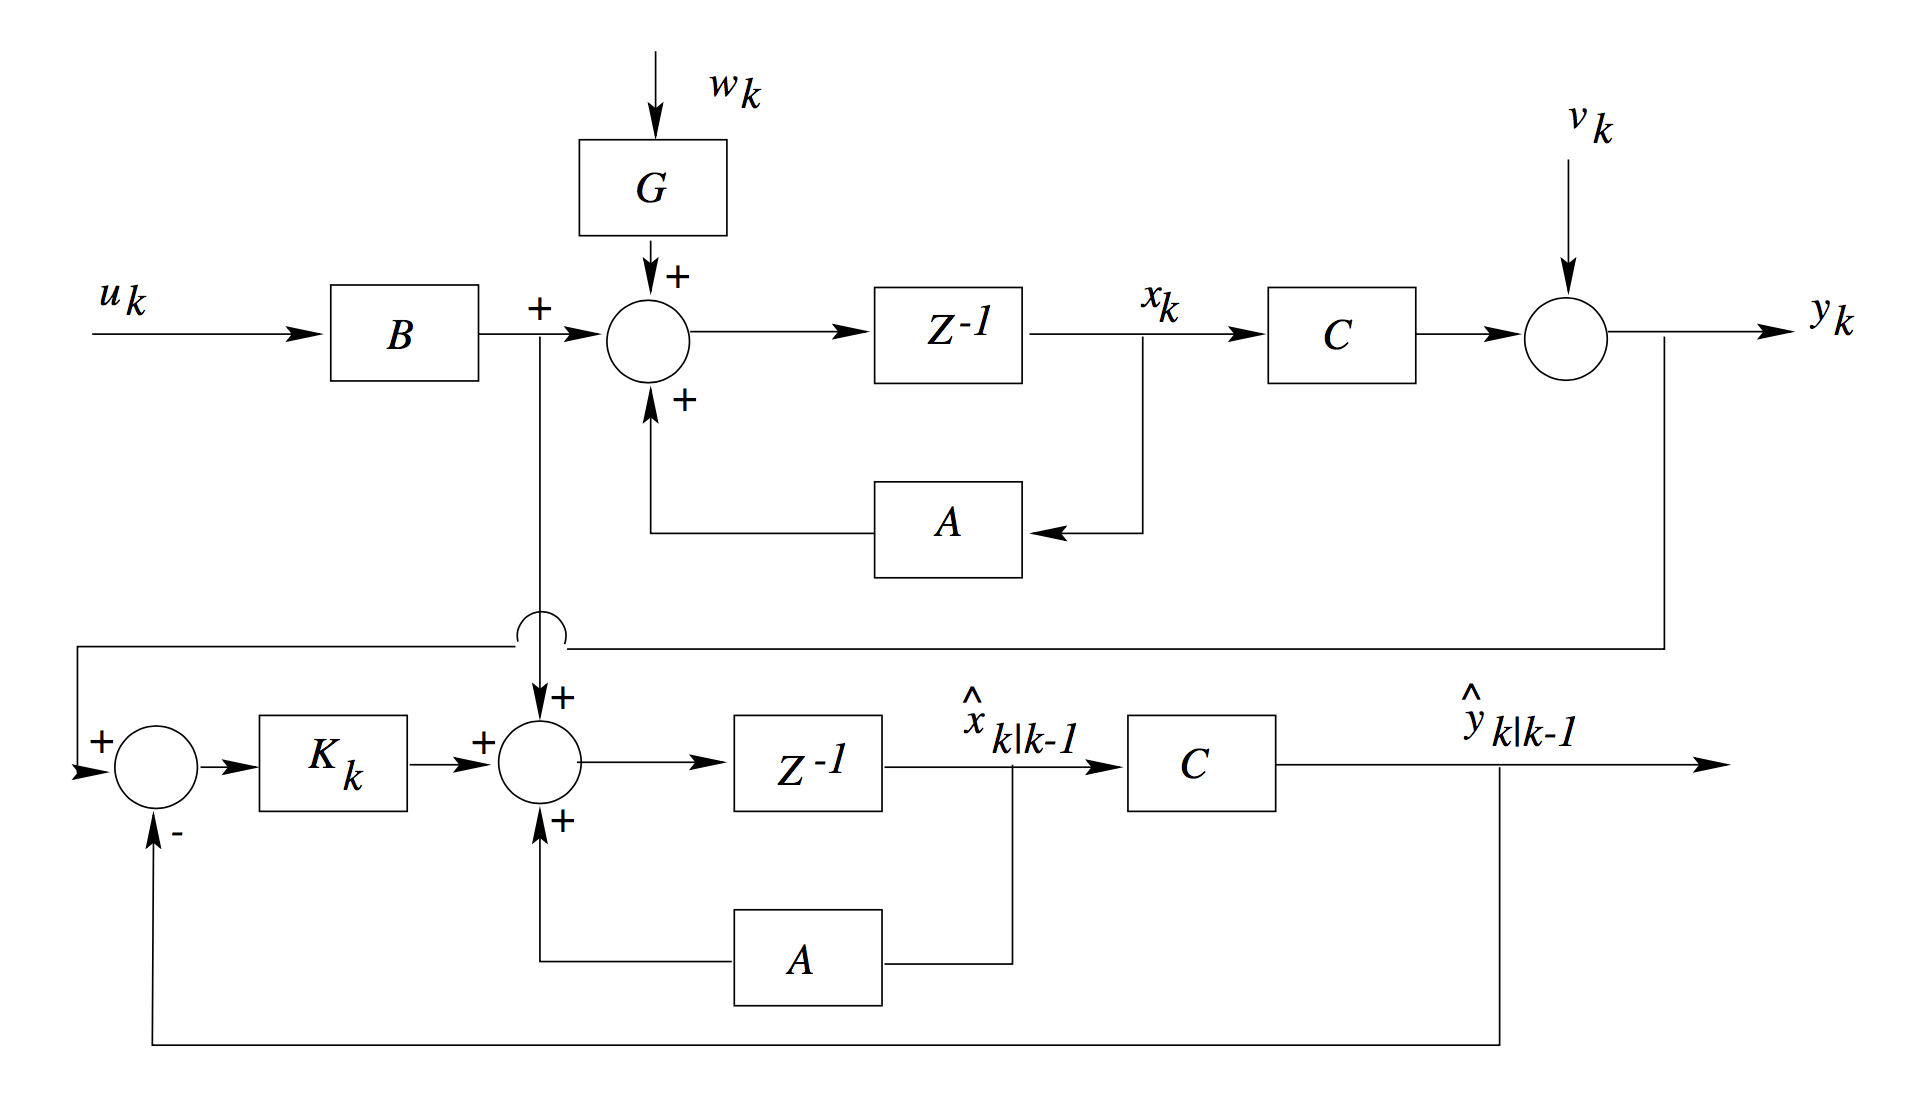
\includegraphics[width=\textwidth]{img/kalmanpred}
	\caption{Schéma-bloc d'un prédicteur de Kalman.}
\end{figure}

\subsubsection{Calcul du filtre de Kalman}
Appliquant de nouveau le Lemme~\ref{lem:orth},
on trouve
\begin{align}
	\xhat_{k \mid k} &= \expe{x_k} + \cov_{x_k \tilde{Z}^k}\cov_{\tilde{Z}^k \tilde{Z}^k}^{-1} \tilde{Z}^k\\
	&= \expe{x_k} + \sum_{j = 0}^k \expe{x_k \ytil_{j \mid j-1}^T} C_{j}^{-1} \ytil_{j \mid j-1}\\
	&= \expe{x_k} + \sum_{j=0}^{k-1} \expe{x_k \ytil_{j \mid j-1}^T} C_j^{-1} \ytil_{j \mid j-1} + \underbrace{\expe{x_k \ytil_{k \mid k-1}^T} C_k^{-1}}_{K_k^{\textnormal{f}}} \ytil_{k \mid k-1}\\
	&= \xhat_{k \mid k-1} + K_k^{\textnormal{f}} \ytil_{k \mid k-1}\,.
\end{align}
Le gain \(K_k^{\textnormal{f}}\) s'obtient comme
\begin{align}
	K_k^{\textnormal{f}} &\triangleq \expe{x_k \ytil_{k \mid k-1}^T} C_k^{-1}\\
	&= \expe{(x_k - \xhat_{k \mid k-1}) \ytil_{k \mid k-1}^T} C_k^{-1}\\
	&= P_{k \mid k-1} C^T C_{k}^{-1}\\
	&= P_{k \mid k-1} C^T (C P_{k \mid k-1} C^T + R)^{-1}\,.
\end{align}
On observe ainsi que
\begin{align}
	K_k &= AK_k^{\textnormal{f}}\,,\\
	\xhat_{k+1 \mid k} &= A \xhat_{x \mid k} + Bu_k\\
	&= A \xhat_{k \mid k-1} + Bu_k + K_k \ytil_{k \mid k-1}\,.
\end{align}

L'erreur de filtrage est donnée par
\begin{equation}
	x_k - \xhat_{k \mid k} = x_k - \xhat_{k \mid k-1} - K_k^{\textnormal{f}} \ytil_{k \mid k-1}\,.
\end{equation}
On trouve donc
\begin{align}
	P_{k \mid k} &\triangleq \expe{(x_k - \xhat_{k \mid k}) (x_k - \xhat_{k \mid k})^T}\\
	&= P_{k \mid k-1} - \expe{\xtil_{k \mid k-1} \ytil_{k \mid k-1}^T} \big(K_k^{\textnormal{f}}\big)^T\\
	&= P_{k \mid k-1} - K_k^{\textnormal{f}} C_k \big(K_k^{\textnormal{f}}\big)^T\\
	&= P_{k \mid k-1} - P_{k \mid k-1} C^T (CP_{k \mid k-1} C^T + R)^{-1} C P_{k \mid k-1}\,.
\end{align}
On observe que l'estimée s'améliore grâce aux nouvelles informations:
\(P_{k \mid k} \le P_{k \mid k-1}\).

On peut alors résumer les équations de filtrage de Kalman comme
\begin{align}
	\xhat_{k \mid k} &= \xhat_{k \mid k-1} + K_k^{\textnormal{f}} \ytil_{k \mid k-1}\,,\\
	K_k^{\textnormal{f}} &= P_{k \mid k-1} C^T (C P_{k \mid k-1} C^T + R)^{-1}\,,\\
	P_{k \mid k} &\triangleq \cov(\xtil_{k \mid k}) = P_{k \mid k-1} - P_{k \mid k-1} C^T (C P_{k \mid k-1} C^T + R)^{-1} C P_{k \mid k-1}\,,
\end{align}
où \(\xhat_{k \mid k-1}\) est calculé à partir du prédicteur de Kalman
et \(P_{k \mid k-1}\) est calculé à partir de l'équation de Riccati.

\subsubsection{Calcul du prédicteur de Kalman à horizon \(j > 1\)}
On cherche maintenant à construire l'estimateur optimal
\(\expe{x_{k + j} \mid Z^k}\) pour \(j > 0\).
À partir de
\begin{equation}
	x_{k+j} = Ax_{k+j-1} + Bu_{k+j-1} + Gw_{k+j-1}
\end{equation}
et l'hypothèse sur \(w_k\), on trouve
\begin{align}
	\xhat_{k+j \mid k} &\triangleq \expe{x_{k+j} \mid Z^k}\\
	&= A \expe{x_{k+j-1} \mid Z^k} + Bu_{k+j-1}\\
	&= A \xhat_{k+j-1 \mid k} + Bu_{k+j-1}\,.
\end{align}
En itérant cette étape \(j\) fois, on trouve
\begin{equation}
	\xhat_{k+j \mid k} = A^j \xhat_{k \mid k} + \sum_{\ell = 0}^{j-1} A^{j - 1 - \ell} Bu_{k + \ell}\,.
\end{equation}
La covariance de l'erreur de ce prédicteur est
\begin{align}
	P_{k+j \mid k} &\triangleq \expe{(x_{k+j} - \xhat_{k+j \mid k})(x_{k+j} - \xhat_{k+j \mid k})^T}\\
	&= \expe{\Big(A(x_{k+j-1} - \xhat_{k+j-1 \mid k}) + Gw_{k+j-1}\Big)\Big(A(x_{k+j-1} - \xhat_{k+j-1 \mid k}) + Gw_{k+j-1}\Big)^T}\\
	&= AP_{k+j-1 \mid k} A^T + GQG^T\\
	&= A^j P_{k \mid k}(A^j)^T + \sum_{\ell = 0}^{j-1} A^\ell GQG^T(A^\ell)^T\,.=
\end{align}

\subsubsection{Lissage optimal}
Le lissage concerne le calcul de \(\expe{x_k \mid Z^j}\), pour \(j < k\).
Il y a trois situations de lissage:
\begin{itemize}
	\item Le \emph{lissage à point fixe}.
	Estimer \(\expe{x_k \mid Z^j}\) pour \(k\) fixé et \(j\) croissant.
	\item Le \emph{lissage à délai fixe}.
	Estimer \(\expe{x_k \mid Z^{k+N}}\) pour tout \(k\) et \(N\) fixé.
	\item Le \emph{lissage à intervalle fixe}.
	Estimer \(\expe{x_k \mid Z^N}\) pour tout \(k\) et \(N\) fixé.
\end{itemize}
Le fait d'utiliser toutes les données, ou au moins quelques données futures,
permet souvent d'améliorer fortement la qualité des estimées.
Cette amélioration dépend du degré de corrélation du signal utile
et du rapport signal/bruit.
Toutes les formules de lissage optimal peuvent être écrites
comme un terme correctif qui vient s'ajouter à la formule du filtre optimal.

On s'intéresse ici au lissage à point fixe.
Considérons le modèle suivant:
\begin{equation}
	\left\{ \begin{array}{rcl} x_{k+1} & = & Ax_k + Gw_k\,,\\
	y_k & = & Cx_k + v_k\,.\end{array}\right.
\end{equation}
On construit \(\xhat_{k \mid j} \triangleq \expe{x_k \mid Z^j}\)
pour un \(k\) aléatoire fixé.
On définit
\begin{equation}
	\xi_j \triangleq \begin{pmatrix} x_j \\ x_j^\textnormal{aug}\end{pmatrix}\,,
\end{equation}
où \(x_j^\textnormal{a} = x_k^\textnormal{aug} = x_k\), pour tout \(j \ge k\).
Le modèle pour cet état augmenté est
\begin{equation}
	\left\{ \begin{array}{rcl} \xi_{j+1} & = & \begin{pmatrix} A & 0 \\ 0 & I \end{pmatrix} \xi_j + \begin{pmatrix} G \\ 0 \end{pmatrix} w_j\,,\quad \xi_k = \begin{pmatrix} x_k \\ x_k \end{pmatrix}\,,\\
	 y_j & = & \begin{pmatrix} C & 0 \end{pmatrix} \xi_j + v_j\,.\end{array}\right.
\end{equation}
Ceci implique donc
\begin{equation}
	\hat{\xi}_{j+1 \mid j} = \begin{pmatrix} \xhat_{j+1 \mid j} \\ \xhat_{k \mid j} \end{pmatrix}\,,
\end{equation}
pour tout \(j \ge k\).

Calculons maintenant le prédicteur de Kalman à horizon \(1\)
pour l'état augmenté \(x_j\).
La partie inférieur de \(\hat{\xi}_{j+1 \mid j}\) est \(\xhat_{k \mid j}\).
On trouve alors
\begin{align}
	\xhat_{k \mid j} &= \xhat_{k \mid k} + \sum_{\ell = k+j}^j K_\ell^{(2)} (y_\ell - C \xhat_{\ell \mid \ell-1})\,,\\
	K_\ell^{(2)} &= P_{\ell \mid \ell-1}^{(21)} C^T (CP_{\ell \mid \ell-1}^{(11)} C^T + R)^{-1}\,.
\end{align}
\(P_{\ell \mid \ell-1}^{(21)}\) et \(P_{\ell \mid \ell-1}^{(11)}\)
sont les sous-matrices de la solution
de l'équation de Riccati pour le système augmenté.
On observe que \(\xhat_{k \mid j}\) est l'estimée filtrée \(\xhat_{k \mid k}\)
à laquelle on a ajouté une somme pondérée des innovations futures.
\begin{align}
	P_{\ell \mid \ell-1} &= \begin{pmatrix} P_{\ell \mid \ell-1}^{(11)} & P_{\ell \mid \ell-1}^{(12)} \\ P_{\ell \mid \ell-1}^{(21)} & P_{\ell \mid \ell-1}^{(22)} \end{pmatrix}\,,
	\intertext{avec}
	P_{\ell+1 \mid \ell} &= \begin{multlined}[t] \begin{pmatrix} A & 0 \\ 0 & I \end{pmatrix} P_{\ell \mid \ell - 1} \begin{pmatrix} A^T & 0 \\ 0 & I \end{pmatrix} + \begin{pmatrix} GQG^T & 0 \\ 0 & 0 \end{pmatrix} - {} \\ \begin{pmatrix} A & 0 \\ 0 & I \end{pmatrix} P_{\ell \mid \ell -1} \begin{pmatrix} C^T \\ 0 \end{pmatrix} \left(\begin{pmatrix} C & 0 \end{pmatrix} P_{\ell \mid \ell - 1} \begin{pmatrix} C^T \\ 0 \end{pmatrix} + R\right)^{-1}\begin{pmatrix} C & 0 \end{pmatrix} P_{\ell \mid \ell - 1} \begin{pmatrix} A^T & 0 \\ 0 & I \end{pmatrix}\,.\end{multlined}
\end{align}

\subsubsection{Prédicteur de Kalman stationnaire}
Le prédicteur de Kalman est un filtre à 2 entrées et une sortie, et s'écrit
\begin{equation}
	\xhat_{k+1 \mid k} = (A - K_k C) \xhat_{k \mid k-1} + Bu_k + K_k y_k\,.
\end{equation}
Pour que ce filtre converge vers un filtre stable à temps invariant,
on requiert que
\begin{align}
	\lim_{k \to +\infty} K_k &= K_{\infty}\,,
	\abs{\lambda_i (A - K_\infty C)} < 1\,, \quad \forall i\,,
\end{align}
où \(K_k = AP_{k \mid k-1} C^T (CP_{k \mid k-1} C^T + R)^{-1}\).

Considérons l'équation de Riccati discrète suivante:
\begin{align}
	P_{k+1 \mid k} &= AP_{k \mid k-1} A^T + GQG^T - AP_{k \mid k-1} C^T (CP_{k \mid k-1} C^T + R)^{-1} CP_{k \mid k-1}A^T\,,\\
	P_{0 \mid -1} &= P_0 \ge 0\,.
\end{align}
Sans perte de généralité, on peut supposer \(Q > 0\).

\begin{mytheo}
	\label{theo:riccaticonv}
	Si \(R > 0\), \((A, G)\) est stabilisable et \((A, C)\) est détectable,\footnote{Ces conditions peuvent encore être relaxées.}
	alors \(\lim_{k \to +\infty} P_{k \mid k-1} = P_{\infty}\),
	where \(P_{\infty}\) est la solution non négative unique
	de l'équation de Riccati algébrique
	\begin{equation}
		P = APA^T + GQG^T - APC^T(CPCP^T + R)^{-1} CPA^T\,.
	\end{equation}
	De plus, \(\abs{\lambda_i (A - K_\infty C)} < 1\) pour tout \(i\),
	avec \(K_\infty = AP_\infty C^T (CP_\infty C^T + R)^{-1}\).
\end{mytheo}
Ici, \((A, G)\) stabilisable signifie qu'il existe une matrice \(L\)
telle que \(\abs{\lambda_i (A - GL)} < 1\), pour tout \(i\),
alors que \((A, C)\) détectable signifie qu'il existe une matrice \(K\)
telle que \(\abs{\lambda_i (A - KC)} < 1\), pour tout \(i\).

Supposons que le gain de Kalman converge vers \(K_\infty\).
On peut alors ré-écrire les équations du prédicteur de Kalman comme
un modèle d'état à temps invariant pour le processus \(y_k\):
\begin{align}
	\xhat_{k+1 \mid k} &= A\xhat_{k \mid k-1} + Bu_k + K_\infty (y_k - \hat{y}_{k \mid k-1})\,,\\
	K_\infty &= AP_\infty C^T (CP_\infty C^T + R)^{-1}\,,\\
	P_\infty &= AP_\infty A^T + GQG^T - AP_\infty C^T (CP_\infty C^T + R)^{-1} CP_\infty A^T\,.
\end{align}
Introduisons la notation \(\varepsilon \triangleq y_k - \hat{y}_{k \mid k-1}\).
Le prédicteur de Kalman peut alors être ré-écrit comme
\begin{equation}
	\left\{ \begin{array}{rcl} \xhat_{k+1 \mid k} & = & A\xhat_{k \mid k-1} + Bu_k + K_\infty \varepsilon_k\,, \\ y_k & = & C\xhat_{k \mid k-1} + \varepsilon_k\,, \end{array}\right.
\end{equation}
avec \(\expe{\varepsilon_k \varepsilon_k^T} = CP_\infty C^T + R\).
Ceci constitue un nouveau modèle pour le processus \(y_k\).
On l'appelle le \emph{modèle d'innovations}.

Supposons que l'on commence avec
un modèle physique stable pour le processus \(y_k\),
excité par deux sources indépendantes de bruit: \(w_k\) et \(v_k\):
\begin{equation}
	\left\{ \begin{array}{rcl} x_{k+1} & = & Ax_k + Bu_k + Gw_k\,, \\ y_k & = & Cx_k + v_k\,.\end{array} \right.
\end{equation}
Grâce au prédicteur de Kalman, on a obtenu un modèle d'innovations pour \(y_k\)
excité par une seule source de bruit \(\varepsilon_k\):
\begin{equation}
	\left\{ \begin{array}{rcl} \xhat_{k+1 \mid k} & = & A\xhat_{k \mid k-1} + Bu_k + K_\infty \varepsilon_k\,, \\ y_k & = & C\xhat_{k \mid k-1} + \varepsilon_k\,. \end{array}\right.
\end{equation}
Les sorties de ces deux modèles
ont la même moyenne et la même fonction de covariance.
Ils sont donc équivalents.

\subsubsection{Modèle d'innovations entrée-sortie: le modèle ARMAX}
L'équation d'entrée-sortie du modèle d'innovations est
\begin{align}
	y_k &= C(zI - A)^{-1} Bu_k + \left(C (zI - A)^{-1} K_\infty + I \right) \varepsilon_k\\
	&= G(z) u_k + H(z) \varepsilon_k\,,
\end{align}
où
\begin{align}
	G(z) &= C(zI - A)^{-1}B\,,\\
	H(z) &= I + C(zI - A)^{-1}K_\infty\,.
\end{align}
Ces deux fonctions de transfert ont les mêmes pôles,
et \(H(z)\) est monique.
Ce modèle est équivalent à un modèle ARMAX:
\begin{equation}
	A(z^{-1})y_k = B(z^{-1})u_k + C(z^{-1})\varepsilon_k\,.
\end{equation}
On a donc justifié la généralité des modèle ARMAX
pour la représentation des processus markoviens linéaires stationnaires,
que ces processus aient plus d'une source de bruit ou non.

Ce modèle a plusieurs propriétés.
On note d'abord
\begin{align}
	\frac{C(z^{-1})}{A(z^{-1})} = H(z) &= I + C(zI - A)^{-1} K_\infty\,,\\
	\frac{B(z^{-1})}{A(z^{-1})} = G(z) &= C(zI - A)^{-1} B\,.
\end{align}
Ceci implique que les racines de \(C(z^{-1})\) sont stables,
car il s'agit des pôles de
\begin{equation}
	\left(I + C(zI - A)^{-1} K_\infty \right)^{-1} = I - C(zI - A + K_\infty C)^{-1} K_\infty\,,
\end{equation}
et que par le Théorème~\ref{theo:riccaticonv},
\(A - K_\infty C\) est une matrice stable.
Le modèle d'innovations est donc inversible de façon stable,
c'est-à-dire que la fonction de transfert
\(H(z)^{-1} = I - C(zI - A + K_\infty C)^{-1} K \)
des observations \(y_k\)
à la séquence d'innovations \(\varepsilon_k\) est stable.
Les séquences \(\{y_j\,, u_j\,, j \le k\}\)
et \(\varepsilon_j\,, u_j\,, j \le k\) contiennent la même information.

\subsubsection{Prédiction à l'aide de modèles ARMAX}
Considérons le modèle ARMAX
\begin{equation}
	A(z^{-1})y_k = B(z^{-1})u_k + C(z^{-1})e_k\,,
\end{equation}
où
\begin{align}
	A(z^{-1}) &\triangleq 1 + a_1z^{-1} + \cdots + a_n z^{-n}\,,\\
	B(z^{-1}) &\triangleq b_1 z^{-1} + \cdots + b_m z^{-m}\,,\\
	C(z^{-1}) &\triangleq 1 + c_1z^{-1} + \cdots + c_p z^{-p}\,,
\end{align}
et \(e_k\) est un bruit blanc centré de variance \(\vars\).
On simplifie en supposant que les processus \(y_k\) et \(u_k\) sont scalaires.
On peut alors construire le meilleur prédicteur à horizon \(1\) de \(y_k\)
étant donné le vecteur de données
\(Z^{k-1} \triangleq \{y_j\,, u_j\,, j \le k-1\}\).
Le modèle ARMAX peut être ré-écrit comme
\begin{equation}
	y_k = \left(1 - A(z^{-1})\right) y_k + B(z^{-1}) u_k + \left(C(z^{-1}) - 1\right) e_k + e_k\,.
\end{equation}
Comme \(C(z)\) est monique et que
\(\{e_j\,, u_j\,, j \le k-1\}\) contient la même information
que \(\{y_j\,, u_j\,, j \le k-1\}\),
le terme \(\left(C(z^{-1}) - 1\right)e_k\) est entièrement connu
au temps \(k-1\).
On trouve donc
\begin{align}
	\hat{y}_{k \mid k-1} &= \expe{y_k \mid Z^{k-1}}\\
	&= \expe{\left(1 - A(z^{-1})\right) y_k + B(z^{-1}) u_k + \left(C(z^{-1} - 1) e_k + e(k) \mid Z^{k-1}\right)}\\
	&= \left(1 - A(z^{-1})\right) y_k + B(z^{-1})u_k + \left(C(z^{-1}) - 1\right)e_k\,.
\end{align}
En remplaçant \(e_k\) ci-dessus par
\(e_k = \frac{A(z^{-1})}{C(z^{-1})} y_k - \frac{B(z^{-1})}{C(z^{-1})}u_k\),
on trouve, après un peu d'algèbre,
\begin{equation}
	C(z^{-1}) \hat{y}_{k \mid k-1} = \left(C(z^{-1}) - A(z^{-1})\right) y_k + B(z^{-1}) u_k\,.
\end{equation}

Le prédicteur à horizon \(1\)
\begin{equation}
	C(z^{-1}) \hat{y}_{k \mid k-1} = \left(C(z^{-1}) - A(z^{-1})\right) y_k + B(z^{-1}) u_k
\end{equation}
doit être interprété comme (avec \(p = n\) pour simplifier)
\begin{align}
	\begin{multlined}[t] \hat{y}_{k \mid k-1} + c_1 \hat{y}_{k-1 \mid k-2} + \cdots + c_n \hat{y}_{k-n \mid k-n-1} = (c_1 - a_1) y_{k-1} + \cdots + (c_n - a_n) y_{k-n} + {} \\ b_1 u_{k-1} + \cdots + b_m u_{k-m}\,.\end{multlined}
\end{align}
On peut également le ré-écrire comme
\begin{equation}
	\hat{y}_{k \mid k-1} = \left(1 - \frac{A(z^{-1})}{C(z^{-1})}\right) y_k + \frac{B(z^{-1})}{C(z^{-1})}u_k\,.
\end{equation}
C'est le prédicteur stationnaire de Kalman optimal pour le modèle ARMAX.

\subsection{Conclusions}
Le filtre de Kalman permet de prédire, de filtrer ou de lisser des estimées
des états d'un système linéaire à temps invariant
sur base des données d'entrée/sortie.
Il procure des estimées optimales basées sur un ensemble fini de données,
en commençant par une condition initiale connue.
En état stationnaire, le filtre de Kalman converge vers un filtre stationnaire
avec un gain constant.
Si le but est de prédire uniquement le signal de sortie futur \(y(t+k)\),
alors on peut calculer le filtre optimal en utilisant un modèle d'entrée/sortie,
sans devoir résoudre d'équation de Riccati.

\appendix
\begin{landscape}
\section{Distributions}
\label{ann:distrib}

\renewcommand{\arraystretch}{1.5}

\begin{table}[h!]
\caption{\label{tab:discrete_dis}Distributions importantes
de variables aléatoires discrètes.}
\begin{tabular}{lcccccc}
\toprule
\multirow{2}{*}{\textbf{Nom}} & \multirow{2}{*}{\textbf{Probabilité}} & \textbf{Densité de} & \textbf{Fonction de} & \multirow{2}{*}{\textbf{Moyenne}} & \multirow{2}{*}{\textbf{Variance}} & \textbf{Fonction} \\
&& \textbf{probabilité} & \textbf{répartition} &&& \textbf{caractéristique}\\
\midrule
 --- & $p_k = \Pr{X = k}$ & $\sum\limits_k p_k \delta(x-k)$ & $\sum\limits_k p_k u(x-k)$ & $\sum\limits_k k p_k$ & $\sum\limits_k (k - \momnc_X)^2 p_k$ & $\sum\limits_k \e^{\imagj nq} p_k$ \\
 \midrule
 & & & & & $a^2p_a(1-p_a)$ & \\
Deux valeurs & $(p_a,p_b)$ & $p_a\delta(x-a) + p_b\delta(x-b)$ & $p_a u(x-a) + p_b u(x-b)$ & $ap_a + bp_b$ & ${}+ b^2p_b(1-p_b)$ & $\e^{\imagj qa}p_a + \e^{\imagj qb}p_b$ \\
&&&&& ${}- 2abp_ap_b$ &\\
\midrule
Binomiale & \multirow{2}{*}{$C_n^kp^k(1-p)^{(n-k)}$} & $\sum\limits_{k=0}^{n} C_n^kp^k(1-p)^{(n-k)}$ & $\sum\limits_{k=0}^{n} C_n^kp^k(1-p)^{(n-k)}$ & \multirow{2}{*}{$np$} & \multirow{2}{*}{$np(1-p)$} & \multirow{2}{*}{$(1-p+p\e^{\imagj q})^n$} \\
$\mathcal B(n,p)$ & & $\delta(x-k)$ & $u(x-k)$ & & & \\
\midrule
Poisson $\mathcal P(\lambda)$  & $\dfrac{\lambda^k e^{-\lambda}}{k!}$ & $\sum\limits_{k=0}^{+\infty} \dfrac{\lambda^k e^{-\lambda}}{k!} \delta(x-k)$ & $\sum\limits_{k=0}^{+\infty} \dfrac{\lambda^k e^{-\lambda}}{k!} u(x-k)$ & $\lambda$ & $\lambda$ & $\e^{-\lambda(\e^{\imagj q}-1)}$\\
\bottomrule
\end{tabular}

\vspace{0.7cm}

\subsection{Propriétés de la distribution de Dirac}
\begin{itemize}
    \item Intégration: $\int_{-\infty}^{+\infty}\delta(x) \dif x = 1$.
    \item Multiplication par une fonction $f$: $f(x)\delta(x-a) = f(a)\delta(x-a)$ pour $a \in \dom f$.
    \item Convolution avec une fonction $f$: $f(x) \ast \delta(x-a) = f(x-a)$.
    \item Relation avec la fonction échelon $u(x)$:
    $\delta(x) = \fdif{}{x}u(x)$.
\end{itemize}
\end{table}

\begin{table}[b!]
\caption{\label{tab:continuous_dis}Distributions importantes
de variables aléatoires continues.}
\begin{tabular}{lccccc}
\toprule
\multirow{2}{*}{\textbf{Nom}} & \textbf{Densité de} & \textbf{Fonction de} & \multirow{2}{*}{\textbf{Moyenne}} & \multirow{2}{*}{\textbf{Variance}} & \textbf{Fonction} \\
& \textbf{probabilité} & \textbf{répartition} &&& \textbf{caractéristique}\\
\midrule
\multirow{2}{*}{---} & \multirow{2}{*}{$\pdf_X(x) = \fdif{\cdf_X(x)}{x}$}
& $\cdf_X(x) = \Pr{X \le x}$
& \multirow{2}{*}{$\int_{-\infty}^{+\infty} x \pdf_X(x) \dif x$}
& \multirow{2}{*}{$\int_{-\infty}^{+\infty} (x - \momnc_X)^2 \pdf_X(x) \dif x$}
& \multirow{2}{*}{$\int_{-\infty}^{+\infty} \e^{\imagj qx} \pdf_X(x) \dif x$}\\
&& $ = \int^{x}_{-\infty} \pdf_X(u) \dif u$ &&&\\
\midrule
\multirow{2}{*}{Uniforme sur $[a,b]$,} & \multirow{3}{*}{$\begin{cases}\displaystyle
                     \frac{1}{b - a} & \text{si } a \le X \le b \\
                     0 & \text{sinon}
	     \end{cases}$}
                     &
                     \multirow{3}{*}{$\begin{cases}
                     0 & \text{si } X \leq a \\\displaystyle
                     \frac{x-a}{b - a} & \text{si } a \leq X \leq b\\
                     1 & \text{si } X > b
	     \end{cases}$}
                     & \multirow{3}{*}{$\frac{a+b}{2}$} & \multirow{3}{*}{$\frac{(b-a)^2}{12}$} & \multirow{3}{*}{$\frac{\e^{\imagj qb} - \e^{\imagj qa}}{\imagj q(b-a)}$} \\
\multirow{2}{*}{$\mathcal U(a,b)$ pour $x\in\R$} & & & & & \\
&&&&& \\
\midrule
\multirow{2}{*}{Normale} &
\multirow{3}{*}{$\frac{1}{\sqrt{2\pi \vars}} \e^{-\frac{(x-\momnc_X)^2}{2\vars_X}}$}
& $1 - \frac{1}{2}\mathrm{erfc}\left( \frac{x-\momnc_X}{\sqrt{2}\sd_X}\right)$
& \multirow{3}{*}{$\momnc_X$}
& \multirow{3}{*}{$\vars_X$}
& \multirow{3}{*}{$\e^{\imagj q\momnc_X} \e^{-\frac{\vars_Xq^2}{2}}$}\\
\multirow{2}{*}{$\mathcal N(\momnc_X,\vars_X)$ pour $x \in \R$} && où &&& \\
&& $\mathrm{erfc}(x) \coloneqq \frac{2}{\sqrt{\pi}} \int_x^{+\infty} \e^{-z^2} \dif z$ &&& \\
\midrule
Rice $\mathcal R(\nu,\sigma)$ &
\multirow{2}{*}{$\frac{x}{\sigma^2}\e^{-\frac{(x^2+\nu^2)}{2\sigma^2}} I_0\left(\frac{x\nu}{\sigma^2}\right)$} & \multirow{2}{*}{Compliqué} & \multirow{2}{*}{Compliqué} & \multirow{2}{*}{Compliqué} & \multirow{2}{*}{Compliqué} \\
pour $x \in [0, +\infty)$ &&&&&\\
\midrule
Rayleigh $\mathcal R(0,\sigma)$ & \multirow{2}{*}{$\frac{x}{\sigma^2} e^{\frac{-x^2}{2 \sigma^2}}$} & \multirow{2}{*}{$1 - \e^{\frac{-x^2}{2 \sigma^2}}$} & \multirow{2}{*}{$ \sigma \sqrt{\frac{\pi}{2}}$} & \multirow{2}{*}{$\frac{4 - \pi}{2} \sigma^2$} & \multirow{2}{*}{Compliqué} \\
pour $x \in [0, +\infty)$ &&&&& \\
\bottomrule
\end{tabular}

\vspace{0.7cm}

$I_0$ est la fonction de Bessel modifiée de première espèce d'ordre zéro.
\end{table}
\end{landscape}

\section{Formules trigonométriques}
Pour rappel,
\begin{align}
	\cos a \cos b &= \frac{1}{2} (\cos(a - b) + \cos(a + b))\\
	\sin a \sin b &= \frac{1}{2} (\cos(a - b) - \cos(a + b))\\
	\sin a \cos b &= \frac{1}{2} (\sin(a - b) + \sin(a + b))
\end{align}

\section{Preuves omises}
\subsection{Formule de la fonction caractéristique}
\label{ann:charfun}
\begin{proof}
\begin{align*}
	\charfun_X(q) &= 1 + \sum_{n=1}^{+\infty} \frac{(\imagj q)^n}{n!}
	\expe{X^n} \\
	&= 1 + \sum_{n=1}^{+\infty} \frac{(\imagj q)^n}{n!}
	\momnc_n \\
	&= 1 + \frac{\imagj q}{1!} \momnc_1 + \frac{(\imagj q)^2}{2!} \momnc_2 + \cdots \\
\end{align*}
Lorsqu'on dérive $n$ fois,
on élimine tous les termes avant le terme en $\momnc_n$.
En évaluant en $q=0$ cette dérivée, on élimine tous ceux après,
car seul le terme en $\momnc_n$ n'a plus de $q$ dans son expression.
On reste donc avec
\begin{align*}
	\left.\fndif{\charfun_X(q)}{q}{n}\right|_{q=0} &= \left.\left(\fndif{q^n}{q}{n} \frac{\imagj^n \momnc_n}{n!}\right)\right|_{q=0} \\
	\left.\fndif{\charfun_X(q)}{q}{n}\right|_{q=0} &= \underbrace{n(n-1)\cdots 1}_{n!} \frac{\imagj^n \momnc_n}{n!}\\
	\implies \momnc_n &= \frac{1}{\imagj^n} \left. \fndif{\charfun_X(q)}{q}{n} \right|_{q=0}\,.\qedhere
\end{align*}
\end{proof}
\end{document}
